% Definiciones y constantes de estilo
% Clase del documento
\documentclass[a4paper,11pt,twoside,openright,titlepage]{book}

%
% Paquetes necesarios
%

\usepackage{eurosym} 			% Símbolo del euro
\usepackage[utf8]{inputenc} 	% Codificación UTF8
\usepackage[spanish,english]{babel} 	% Caracteres del español
\usepackage{listings} 		% Código, algoritmos, etc.
\usepackage{color} 			% Definición de colores
\usepackage[table,xcdraw]{xcolor} 		% Extensión del paquete color
\usepackage{anysize} 		% Márgenes
\usepackage{fancyhdr} 		% Cabecera y pie de página
\usepackage{quotchap} 		% Estilo título capítulos
\usepackage{algorithmic} 	% Algoritmos (expresarlos mejor)
\usepackage{titlesec} 		% Títulos de secciones
\usepackage{amsmath} 		% Fórmulas matemáticas
\usepackage{enumerate} 		% Enumeraciones
\usepackage{emptypage} 		% Páginas en blanco
\usepackage{float} 			% Separación entre cajas
\usepackage{graphicx} 		% Imágenes
\usepackage{array} 			% Mejora de las tablas
\usepackage{mdwmath} 		% Mejora de los símbolos matemáticos
\usepackage[caption=false,font=footnotesize]{subfig} 		% Separar figuras en subfiguras
\usepackage{pdfpages} 		% Incluir pdfs externos
\usepackage{fancybox} 		% Mejoras sobre las cajas
\usepackage{appendix} 		% Apéndices
\usepackage{bookmark} 		% Marcadores (para el pdf)
\usepackage{enumitem} 		% Estilo de enumeraciones
\usepackage{setspace} 		% Espacio entre líneas y párrafos
\usepackage[acronym]{glossaries} 		% Glosario/Acrónimos
\usepackage[T1]{fontenc} 	% Fuentes
\usepackage[sorting=none,natbib=true,backend=bibtex,bibencoding=ascii]{biblatex} 		% Bibliografía
\usepackage{csquotes} 		% Fix biblatex+babel warning
\usepackage{exmath}
\usepackage{MathUnicode}
\usepackage{imakeidx}
\usepackage{definitions}
\usepackage{breqn}
\usepackage{hyperref}

\usepackage{babel}

\usetikzlibrary{arrows}
\tikzset{
every picture/.append style={
  execute at begin picture={\deactivatequoting},
  execute at end picture={\activatequoting}
  }
}
%\tikzset{every node/.append style={minimum size=0.5cm, draw,circle,font=\sffamily\Large\bfseries,inner sep=0.05cm}}%



%\PrerenderUnicode{ÁáÉéÍíÓóÚúÑñ} % Para que salgan las tildes y demás mierdas en el título.

% Enlaces
\hypersetup{hidelinks,pageanchor=true,colorlinks,citecolor=Fuchsia,urlcolor=black,linkcolor=Cerulean}

% Euro (€)
\DeclareUnicodeCharacter{20AC}{\euro}

% Inclusión de gráficos
\graphicspath{{./graphics/}}

% Extensiones de gráficos
\DeclareGraphicsExtensions{.pdf,.jpeg,.jpg,.png}

% Definiciones de colores (para hidelinks)
\definecolor{LightCyan}{rgb}{0,0,0}
\definecolor{Cerulean}{rgb}{0,0,0}
\definecolor{Fuchsia}{rgb}{0,0,0}

% Keywords (español e inglés)
\def\keywordsEn{\vspace{.5em}
{\textbf{\textit{Key words ---}}\,\relax%
}}
\def\endkeywordsEn{\par}

\def\keywordsEs{\vspace{.5em}
{\textbf{\textit{Palabras clave ---}}\,\relax%
}}
\def\endkeywordsEs{\par}


% Abstract (español e inglés)
\def\abstractEs{\vspace{.5em}
{\textbf{\textit{Resumen ---}}\,\relax%
}}
\def\endabstractEs{\par}

\def\abstractEn{\vspace{.5em}
{\textbf{\textit{Abstract ---}}\,\relax%
}}
\def\endabstractEn{\par}

% Estilo páginas de capítulos
\fancypagestyle{plain}{
\fancyhf{}
\fancyfoot[CO]{\footnotesize\emph{\workname}}
\fancyfoot[RO]{\thepage}
\renewcommand{\footrulewidth}{.6pt}
\renewcommand{\headrulewidth}{0.0pt}
}

% Estilo resto de páginas
\pagestyle{fancy}

% Estilo páginas impares
\fancyfoot[CO]{\footnotesize\emph{\workname}}
\fancyfoot[RO]{\thepage}
\rhead[]{\leftmark}

% Estilo páginas pares
\fancyfoot[CE]{\emph{\pieparcen}}
\fancyfoot[LE]{\thepage}
\fancyfoot[RE]{\pieparizq}
\lhead[\leftmark]{}

% Guía del pie de página
\renewcommand{\footrulewidth}{.6pt}

% Nombre de los bloques de código
\renewcommand{\lstlistingname}{Code}

% Estilo de los lstlistings
\lstset{
    frame=tb,
    breaklines=true,
    postbreak=\raisebox{0ex}[0ex][0ex]{\ensuremath{\color{gray}\hookrightarrow\space}}
}

% Definiciones de funciones para los títulos
\newlength\salto
\setlength{\salto}{3.5ex plus 1ex minus .2ex}
\newlength\resalto
\setlength{\resalto}{2.3ex plus.2ex}

% Estilo de los acrónimos

\pretolerance=2000
\tolerance=3000

% Texto índice de tablas
%\addto\captionsspanish{
%\def\tablename{Tabla}
%\def\listtablename{\'Indice de tablas}
%}


% Comando code (lstlisting sin cambio de página)
\lstnewenvironment{code}[1][]%
  { \noindent\minipage{0.935\linewidth}\medskip
    \vspace{5mm}
    \lstset{basicstyle=\ttfamily\footnotesize,#1}}
  {\endminipage}

%\newcommand{\implies}{\rightarrow}
%\newcommand{\impliedby}{\leftarrow}
%\newcommand{\dimplies}{\leftrightarrow}
\newcommand{\orcond}{\vee}
\newcommand{\andcond}{\wedge}
\newcommand{\true}{\top}
\newcommand{\false}{\perp}
\newcommand{\axioms}{\mathcal{A}}

% % % % From Alejandro Sánchez
	\newcommand{\figscale}{0.36}
	\newcommand{\funcscale}{0.34}
	\newcommand{\queuescale}{0.32}
	\newcommand{\leapscale}{0.42}
	\newcommand{\listscale}{0.30}
	\newcommand{\robotscale}{0.28}
	\newcommand{\longtablesize}{22em}
	\newcommand{\medtablesize}{25em}
	\newcommand{\smalltablesize}{6em}
	\newcommand{\intersize}{30em}
	\newcommand{\quadsize}{\quad}

\renewcommand{\pc}{pc}
\newcommand{\tbf}[1]{\textbf{#1}}



%%%%%%%%%%%%%%%%%%%%%%%%%%%%%%%%%%%%%%
%%                                  %%
%%  Basic terminology for theories  %%
%%                                  %%
%%%%%%%%%%%%%%%%%%%%%%%%%%%%%%%%%%%%%%

%% Signatures
\newcommand{\Sig}{\ensuremath{\Sigma}\xspace}
\newcommand{\SigInter}{\ensuremath{\Sig}-interpretation\xspace}
\newcommand{\SigStruct}{\ensuremath{\Sig}-structure\xspace}
\newcommand{\SigStructs}{\ensuremath{\Sig}-structures\xspace}
\newcommand{\SigTerm}{\ensuremath{\Sig}-term\xspace}
\newcommand{\SigFormula}{\ensuremath{\Sig}-formula\xspace}
\newcommand{\SigLiteral}{\ensuremath{\Sig}-literal\xspace}
\newcommand{\SigTheory}{\ensuremath{\Sig}-theory\xspace}
\newcommand{\SigFormulaSet}{\ensuremath{F_{\Sig}}\xspace}
\newcommand{\SigFormulaSetVar}[1]{\ensuremath{F_{\Sig}^{(#1)}}\xspace}

%% Interpretations
\newcommand{\Omg}{\ensuremath{\Omega}\xspace}
\newcommand{\OmgInter}{\ensuremath{\Omg}-interpretation\xspace}
\newcommand{\AiSig}{\ensuremath{\Ai^{\Sig}}\xspace}
\newcommand{\SigClass}{\ensuremath{\mathbf{A}}\xspace}

% Variable sets
\newcommand{\VarV}{\ensuremath{V}\xspace}
\newcommand{\VarU}{\ensuremath{U}\xspace}

%% Generic theories names
\newcommand{\Theo}{\ensuremath{T}\xspace}
\newcommand{\TheoInter}{\ensuremath{\Theo}-interpretation\xspace}
\newcommand{\TheoSat}{\ensuremath{\Theo}-satisfiable\xspace}


%% Symbols for theory combination
\newcommand{\sort}{\ensuremath{\mathit{sort}}\xspace}


%% Theory names
\newcommand{\addr}{\ensuremath{\mathsf{addr}}\xspace}
\newcommand{\elem}{\ensuremath{\mathsf{elem}}\xspace}
\newcommand{\tid}{\ensuremath{\mathsf{tid}}\xspace}
\newcommand{\thId}{\ensuremath{\mathsf{tid}}\xspace}
\newcommand{\cell}{\ensuremath{\mathsf{cell}}\xspace}
\newcommand{\cells}{\ensuremath{\mathsf{cell}}\xspace}
\newcommand{\cellsK}{\ensuremath{\mathsf{cell}_{\mathsf{K}}}\xspace}
\newcommand{\memory}{\ensuremath{\mathsf{mem}}\xspace}
\newcommand{\mem}{\ensuremath{\mathsf{mem}}\xspace}
\newcommand{\memoryK}{\ensuremath{\mathsf{mem}_{\mathsf{K}}}\xspace}
%\newcommand{\reach}{\ensuremath{\mathsf{reachability}}\xspace}
\newcommand{\reach}{\ensuremath{\mathsf{reach}}\xspace}
\newcommand{\reachK}{\ensuremath{\mathsf{reach}_{\mathsf{K}}}\xspace}
\providecommand*{\path}{}
\renewcommand{\path}{\ensuremath{\mathsf{path}}\xspace}
\newcommand{\bridge}{\ensuremath{\mathsf{bridge}}\xspace}
\newcommand{\bridgeK}{\ensuremath{\mathsf{bridge}_{\mathsf{K}}}\xspace}
\newcommand{\lists}{\ensuremath{\mathsf{Lists}}\xspace}
\newcommand{\cons}{\ensuremath{\mathsf{cons}}\xspace}
\newcommand{\listsBridge}{\ensuremath{\mathsf{ListsBridge}}\xspace}


%% Sorts
\newcommand{\sTID}{\textsf{tid}\xspace}
\newcommand{\sBool}{\ensuremath{\mathsf{boolean}}\xspace}
\newcommand{\sElem}{\ensuremath{\mathsf{elem}}\xspace}
\newcommand{\sAddr}{\ensuremath{\mathsf{addr}}\xspace}
\newcommand{\sTid}{\ensuremath{\mathsf{tid}}\xspace}
\newcommand{\sCell}{\ensuremath{\mathsf{cell}}\xspace}
\newcommand{\sCellK}{\ensuremath{\cellsK}\xspace}
\newcommand{\sMem}{\ensuremath{\mathsf{mem}}\xspace}
\newcommand{\sMemK}{\ensuremath{\memoryK}\xspace}
\newcommand{\sPath}{\ensuremath{\mathsf{path}}\xspace}
\newcommand{\sWhatever}{\ensuremath{\mathsf{\_}}\xspace}
\newcommand{\sSetWhatever}{\ensuremath{\mathsf{set}}\sWhatever\xspace}
\newcommand{\sSetAddr}{\ensuremath{\mathsf{setaddr}}\xspace}
\newcommand{\sSetElem}{\ensuremath{\mathsf{setelem}}\xspace}
\newcommand{\sSetTid}{\ensuremath{\mathsf{settid}}\xspace}
\newcommand{\sSet}{\ensuremath{\mathsf{setaddr}}\xspace}
\newcommand{\sSetE}{\ensuremath{\mathsf{setelem}}\xspace}
\newcommand{\sSetT}{\ensuremath{\mathsf{settid}}\xspace}
\newcommand{\sSeq}{\ensuremath{\mathsf{fseq}}\xspace}
\newcommand{\sList}{\ensuremath{\mathsf{list}}\xspace}
\newcommand{\sArray}{\ensuremath{\mathsf{array}}\xspace}
\newcommand{\sCList}{\ensuremath{\mathsf{clist}}\xspace}
\newcommand{\sLevel}{\ensuremath{\mathsf{level}}\xspace}
\newcommand{\sLevelK}{\ensuremath{\mathsf{level}_{\mathsf{K}}}\xspace}
\newcommand{\sOrd}{\ensuremath{\mathsf{ord}}\xspace}
\newcommand{\sAArray}{\ensuremath{\mathsf{aarr}}\xspace}
\newcommand{\sLArray}{\ensuremath{\mathsf{larr}}\xspace}
\newcommand{\sPair}{\ensuremath{\mathsf{pair}}\xspace}
\newcommand{\sSetPair}{\ensuremath{\mathsf{setpair}}\xspace}
\newcommand{\sMrgn}{\ensuremath{\mathsf{mrgn}}\xspace}
\newcommand{\sLock}{\ensuremath{\mathsf{sem}}\xspace}


%% Functions
\newcommand{\fNil}{\ensuremath{\mathit{nil}}\xspace}
\newcommand{\fCons}{\ensuremath{\mathit{cons}}\xspace}
\newcommand{\fHd}{\ensuremath{\mathit{hd}}\xspace}
\newcommand{\fTl}{\ensuremath{\mathit{tl}}\xspace}
\newcommand{\fError}{\ensuremath{\mathit{error}}\xspace}
\newcommand{\fMkcell}{\ensuremath{\mathit{mkcell}}\xspace}
\newcommand{\fData}{\ensuremath{\mathit{data}}\xspace}
\newcommand{\fSem}{\ensuremath{\mathit{lock}}\xspace}
\newcommand{\fKey}{\ensuremath{\mathit{key}}\xspace}
\newcommand{\fNext}{\ensuremath{\mathit{next}}\xspace}
\newcommand{\fOrderlist}{\ensuremath{\mathit{orderlist}}\xspace}
\newcommand{\fMalloc}{\ensuremath{\mathit{malloc}}\xspace}
\newcommand{\fLockID}{\ensuremath{\mathit{lockid}}\xspace}
\newcommand{\fLock}{\ensuremath{\mathit{lock}}\xspace}
\newcommand{\fUnlock}{\ensuremath{\mathit{unlock}}\xspace}
\newcommand{\fNull}{\ensuremath{\mathit{null}}\xspace}
\newcommand{\fNoThread}{\ensuremath{\oslash}\xspace}
\newcommand{\fUndef}{\ensuremath{\mathit{undef}}\xspace}
\newcommand{\fRd}{\ensuremath{\mathit{rd}}\xspace}
\newcommand{\fUpd}{\ensuremath{\mathit{upd}}\xspace}
\newcommand{\fRev}{\ensuremath{\mathit{rev}}\xspace}
\newcommand{\fEpsilon}{\ensuremath{\epsilon}\xspace}
\newcommand{\fPathToSet}{\ensuremath{\mathit{path2set}}\xspace}
\newcommand{\fPathToSetA}{\ensuremath{\mathit{\inter{path2set}{\Ai}}}\xspace}
\newcommand{\fPathToSetB}{\ensuremath{\mathit{\inter{path2set}{\Bi}}}\xspace}
\newcommand{\fSetToElemSet}{\ensuremath{\mathit{set2elemset}}\xspace}
\newcommand{\fAddrToSet}{\ensuremath{\mathit{addr2set}}\xspace}
\newcommand{\fAddrToSetK}{\ensuremath{\mathit{addr2set_{\K}}}\xspace}
\newcommand{\fGetp}{\ensuremath{\mathit{getp}}\xspace}
\newcommand{\fGetpK}{\ensuremath{\mathit{getp_{\K}}}\xspace}
\newcommand{\fPathToList}{\ensuremath{\mathit{path2list}}\xspace}
\newcommand{\fPathToListA}{\ensuremath{\inter{\fPathToList}{\Ai}}\xspace}
\newcommand{\fPathToListB}{\ensuremath{\inter{\fPathToList}{\Bi}}\xspace}
\newcommand{\fPathToCList}{\ensuremath{\mathit{path2clist}}\xspace}
\newcommand{\fPathToCListA}{\ensuremath{\inter{\fPathToCList}{\Ai}}\xspace}
\newcommand{\fPathToCListB}{\ensuremath{\inter{\fPathToCList}{\Bi}}\xspace}
%\newcommand{\fFirstLocked}{\ensuremath{\mathit{firstlocked}}\xspace}
\newcommand{\fFirstLocked}{\ensuremath{\mathit{fstlock}}\xspace}
\newcommand{\fLastLocked}{\ensuremath{\mathit{lstlock}}\xspace}
%\newcommand{\fFirstLockedK}{\ensuremath{\mathit{firstlocked_{\K}}}\xspace}
\newcommand{\fFirstLockedK}{\ensuremath{\mathit{fstlock_{\K}}}\xspace}
\newcommand{\fThreadSubset}{\ensuremath{\mathit{thSubset}}\xspace}
\newcommand{\fMinTh}{\ensuremath{\mathit{minTh}}\xspace}
\newcommand{\fMin}{\ensuremath{\mathit{min}}\xspace}

\newcommand{\fLUKSubset}{\ensuremath{\mathit{subset_{\mathit{LUH}}}}\xspace}
\newcommand{\fInterLUK}{\ensuremath{\mathit{inter_{\mathit{LUH}}}}\xspace}
\newcommand{\fEmptyLUK}{\ensuremath{\mathit{empty_{\mathit{LUH}}}}\xspace}
\newcommand{\fMinLUK}{\ensuremath{\mathit{min_{\mathit{LUH}}}}\xspace}


\newcommand{\fListToSet}{\ensuremath{\mathit{list2set}}\xspace}
\newcommand{\fListToSetA}{\ensuremath{\inter{\fListToSet}{\Ai}}\xspace}
\newcommand{\fListToSetB}{\ensuremath{\inter{\fListToSet}{\Bi}}\xspace}
\newcommand{\fSeqToList}{\ensuremath{\mathit{fseq2list}}\xspace}
\newcommand{\fSeqToCList}{\ensuremath{\mathit{fseq2clist}}\xspace}
%\newcommand{\fFirstMarked}{\ensuremath{\mathit{firstmarked}}\xspace}
\newcommand{\fFirstMarked}{\ensuremath{\mathit{fstmark}}\xspace}
\newcommand{\fIsPath}{\ensuremath{\mathit{ispath}}\xspace}
\newcommand{\fLevel}[1]{\ensuremath{\eta_{#1}}\xspace}
\newcommand{\fZero}{\ensuremath{0}\xspace}
\newcommand{\fMinusInfty}{\ensuremath{-\infty}\xspace}
\newcommand{\fInfty}{\ensuremath{+\infty}\xspace}
\newcommand{\fSucc}{\ensuremath{\mathsf{succ}}\xspace}
\newcommand{\fSkipKToList}{\ensuremath{\mathit{skiplist_{\mathsf{k}}2list}}\xspace}
\newcommand{\fApp}{\ensuremath{\mathit{app}}\xspace}
\newcommand{\fSeqToSet}{\ensuremath{\mathit{fseq2set}}\xspace}
\newcommand{\fLast}{\ensuremath{\mathit{last}}\xspace}
\newcommand{\fCont}{\ensuremath{\mathit{cont}}\xspace}
\newcommand{\pContAtLevelK}{\ensuremath{\mathit{cont_{\K}}}\xspace}
\newcommand{\pContAtLevel}{\ensuremath{\mathit{contAtLevel}}\xspace}
\newcommand{\fPair}[2]{\ensuremath{\langle{#1},{#2}\rangle}\xspace}

\newcommand{\fSingl}{\ensuremath{\mathit{singl}}\xspace}
\newcommand{\fUnion}{\ensuremath{\mathit{Union}}\xspace}
\newcommand{\fSetdiff}{\ensuremath{\mathit{setDiff}}\xspace}
\newcommand{\fEmptyset}{\ensuremath{\mathit{emptyset}}\xspace}
\newcommand{\pIn}{\ensuremath{\mathit{in}}\xspace}

\newcommand{\fSinglElem}{\ensuremath{\mathit{singlElem}}\xspace}
\newcommand{\fUnionElem}{\ensuremath{\mathit{UnionElem}}\xspace}
\newcommand{\fSetdiffElem}{\ensuremath{\mathit{setDiffElem}}\xspace}
\newcommand{\fEmptysetElem}{\ensuremath{\mathit{emptysetElem}}\xspace}
\newcommand{\pInElem}{\ensuremath{\mathit{inElem}}\xspace}

\newcommand{\fSinglTid}{\ensuremath{\mathit{singlTh}}\xspace}
\newcommand{\fUnionTid}{\ensuremath{\mathit{UnionTh}}\xspace}
\newcommand{\fSetdiffTid}{\ensuremath{\mathit{setDiffTh}}\xspace}
\newcommand{\fEmptysetTid}{\ensuremath{\mathit{emptysetTh}}\xspace}
\newcommand{\pInTid}{\ensuremath{\mathit{inTh}}\xspace}

\newcommand{\fHighest}{\ensuremath{\mathit{highestElem}}\xspace}
\newcommand{\fLowest}{\ensuremath{\mathit{lowestElem}}\xspace}
\newcommand{\fLselem}{\ensuremath{\mathit{ls\_elem}}\xspace}


%% Operations for the generic array manipulation
\newcommand{\fArrayRd}[2]
		{\ensuremath{{#1} \lbrack {#2} \rbrack}\xspace}
\newcommand{\fArrayUpd}[3]
		{\ensuremath{{#1} \{{#2} \gets {#3} \}}\xspace}
\newcommand{\fArrayRdInter}[3]
		{\ensuremath{{#1} \lbrack {#2} \rbrack^{#3}}\xspace}
\newcommand{\fArrayUpdInter}[4]
		{\ensuremath{{#1} \{{#2} \gets {#3} \}^{#4}}\xspace}

\newcommand{\contained}{\ensuremath{\mathit{contained}}\xspace}


%% Predicates
\newcommand{\pOrdPath}{\ensuremath{\mathit{ordPath}}\xspace}
\newcommand{\pOrdList}{\ensuremath{\mathit{ordList}}\xspace}
\newcommand{\pSubPath}{\ensuremath{\mathit{subPath}}\xspace}
\newcommand{\pAppend}{\ensuremath{\mathit{append}}\xspace}
\newcommand{\pReach}{\ensuremath{\mathit{reach}}\xspace}
\newcommand{\pReachK}{\ensuremath{\mathit{reach_{\K}}}\xspace}
%\newcommand{\pIsReachable}{\eniguremath{\mathit{isreachable}}\xspace}
\newcommand{\pIsReachable}{\eniguremath{\mathit{isreach}}\xspace}
\newcommand{\pOrd}{\ensuremath{\preceq}\xspace}
\newcommand{\pStrictOrd}{\ensuremath{\prec}\xspace}
\newcommand{\pSubList}{\ensuremath{\mathit{SubList}}\xspace}
\newcommand{\pSkiplistK}{\ensuremath{\mathit{Skiplist_{\mathsf{K}}}}\xspace}
\newcommand{\pDisjLevelK}{\ensuremath{\mathit{DisjLevel_{\mathsf{K}}}}\xspace}
%\newcommand{\pIsReach}{\ensuremath{\mathit{isreachable}}\xspace}
\newcommand{\pIsReach}{\ensuremath{\mathit{isreach}}\xspace}
%\newcommand{\pIsReachP}{\ensuremath{\mathit{isreachablep}}\xspace}
\newcommand{\pIsReachP}{\ensuremath{\mathit{isreachp}}\xspace}
%\newcommand{\pIsReachK}{\ensuremath{\mathit{isreachable_{\K}}}\xspace}
\newcommand{\pIsReachK}{\ensuremath{\mathit{isreach_{\K}}}\xspace}
%\newcommand{\pIsReachKP}{\ensuremath{\mathit{isreachablep_{\K}}}\xspace}
\newcommand{\pIsReachKP}{\ensuremath{\mathit{isreachp_{\K}}}\xspace}

\newcommand{\pInTidPair}{\ensuremath{\mathit{inTidPair}}\xspace}
\newcommand{\pUniqueInt}{\ensuremath{\mathit{uniqueInt}}\xspace}
\newcommand{\pUniqueTid}{\ensuremath{\mathit{uniqueTid}}\xspace}



%% Signatures
\newcommand{\sigAddr}{\ensuremath{\Sigma_{\addr}}\xspace}
\newcommand{\sigElem}{\ensuremath{\Sigma_{\elem}}\xspace}
\newcommand{\sigTid}{\ensuremath{\Sigma_{\thId}}\xspace}
\newcommand{\sigCells}{\ensuremath{\Sigma_{\cells}}\xspace}
\newcommand{\sigCellsK}{\ensuremath{\Sigma_{\cellsK}}\xspace}
\newcommand{\sigMemory}{\ensuremath{\Sigma_{\memory}}\xspace}
\newcommand{\sigMemoryK}{\ensuremath{\Sigma_{\memoryK}}\xspace}
\newcommand{\sigReach}{\ensuremath{\Sigma_{\reach}}\xspace}
\newcommand{\sigReachK}{\ensuremath{\Sigma_{\reachK}}\xspace}
\newcommand{\sigSets}{\ensuremath{\Sigma_{\sSet}}\xspace}
\newcommand{\sigSetsE}{\ensuremath{\Sigma_{\sSetE}}\xspace}
\newcommand{\sigSetsT}{\ensuremath{\Sigma_{\sSetT}}\xspace}
\newcommand{\sigBridge}{\ensuremath{\Sigma_{\bridge}}\xspace}
\newcommand{\sigBridgeK}{\ensuremath{\Sigma_{\bridgeK}}\xspace}
\newcommand{\sigLists}{\ensuremath{\Sigma_{\cons}}\xspace}
\newcommand{\sigListsBridge}{\ensuremath{\Sigma_{\listsBridge}}\xspace}
\newcommand{\sigSeq}{\ensuremath{\Sigma_{\sSeq}}\xspace}
\newcommand{\sigPath}{\ensuremath{\Sigma_{\sPath}}\xspace}
\newcommand{\sigMrgn}{\ensuremath{\Sigma_{\sMrgn}}\xspace}
\newcommand{\sigTLL}{\ensuremath{\Sigma_{\TLL}}\xspace}
\newcommand{\sigTLLh}{\ensuremath{\Sigma_{\TLLh}}\xspace}
\newcommand{\sigTLLpL}{\ensuremath{\Sigma_{\TLLpL}}\xspace}
\newcommand{\sigTLLpLh}{\ensuremath{\Sigma_{\TLLpLh}}\xspace}
\newcommand{\sigLevel}{\ensuremath{\Sigma_{\sLevel}}\xspace}
\newcommand{\sigLevelK}{\ensuremath{\Sigma_{\sLevelK}}\xspace}
\newcommand{\sigOrd}{\ensuremath{\Sigma_{\sOrd}}\xspace}
\newcommand{\sigBasepL}{\ensuremath{\Sigma_{\textsf{Base3}}}\xspace}
\newcommand{\sigAArray}{\ensuremath{\Sigma_{\sAArray}}\xspace}
\newcommand{\sigLArray}{\ensuremath{\Sigma_{\sLArray}}\xspace}
\newcommand{\sigPair}{\ensuremath{\Sigma_{\sPair}}\xspace}
\newcommand{\sigSetPair}{\ensuremath{\Sigma_{\sSetPair}}\xspace}
\newcommand{\sigLUK}{\ensuremath{\Sigma_{\mathsf{LUH}}}\xspace}
\newcommand{\sigTSLK}{\ensuremath{\Sigma_{\TSLK}}\xspace}
\newcommand{\sigTSLKh}{\ensuremath{\Sigma_{\TSLKh}}\xspace}
\newcommand{\sigTSLKhBar}{\ensuremath{\Sigma_{\TSLKhBar}}\xspace}
\newcommand{\sigTBaseSLK}{\ensuremath{\Sigma_{\TBaseSLK}}\xspace}
\newcommand{\sigTBaseSLKP}{\ensuremath{\Sigma_{\TBaseSLKP}}\xspace}


%% Interpretations
\newcommand{\interTLL}{\ensuremath{\textbf{TLL}}\xspace}
\newcommand{\interTLLpL}{\ensuremath{\textbf{TL3}}\xspace}
\newcommand{\interTOrd}{\ensuremath{\textbf{TOrd}}\xspace}
\newcommand{\interTSLK}{\ensuremath{\textbf{TSLK}}\xspace}


%% Theories
\newcommand{\thCells}{\ensuremath{\mathit{T}_{\cells}}\xspace}
\newcommand{\thElem}{\ensuremath{\mathit{T}_{\elem}}\xspace}
\newcommand{\thTid}{\ensuremath{\mathit{T}_{\thId}}\xspace}
\newcommand{\thAddr}{\ensuremath{\mathit{T}_{\addr}}\xspace}
\newcommand{\thMem}{\ensuremath{\mathit{T}_{\memory}}\xspace}
\newcommand{\thReach}{\ensuremath{\mathit{T}_{\reach}}\xspace}
\newcommand{\thPath}{\ensuremath{\mathit{T}_{\path}}\xspace}
\newcommand{\thSets}{\ensuremath{\mathit{T}_{\sets}}\xspace}
\newcommand{\thSetsE}{\ensuremath{\mathit{T}_{\setsE}}\xspace}
\newcommand{\thSetsT}{\ensuremath{\mathit{T}_{\setsT}}\xspace}
\newcommand{\thSeq}{\ensuremath{\mathit{T}_{\sSeq}}\xspace}
\newcommand{\thLists}{\ensuremath{\mathit{T}_{\cons}}\xspace}
\newcommand{\thMrgn}{\ensuremath{\mathit{T}_{\sMrgn}}\xspace}
\newcommand{\thAArray}{\ensuremath{\mathit{T}_{\sAArray}}\xspace}
\newcommand{\thLArray}{\ensuremath{\mathit{T}_{\sLArray}}\xspace}
\newcommand{\thLUK}{\ensuremath{\mathit{T}_{\mathsf{LUH}}}\xspace}
\newcommand{\thPair}{\ensuremath{\mathit{T}_{\sPair}}\xspace}
\newcommand{\thSetPair}{\ensuremath{\mathit{T}_{\sSetPair}}\xspace}
\newcommand{\thBridge}{\ensuremath{\mathit{T}_{\bridge}}\xspace}

\newcommand{\TLL}{\ensuremath{\textsf{TLL}}\xspace}
\newcommand{\TLLh}{\ensuremath{\widehat{\textsf{TLL}}}\xspace}
\newcommand{\TLLpL}{\ensuremath{\textsf{TL3}}\xspace}
\newcommand{\TLLpLh}{\ensuremath{\widehat{\textsf{TL3}}}\xspace}
\newcommand{\TBase}{\ensuremath{\mathit{T}_{\textsf{Base}}}\xspace}
\newcommand{\TBasepL}{\ensuremath{\mathit{T}_{\textsf{Base3}}}\xspace}
\newcommand{\TBaseSLK}{\ensuremath{\mathit{T}_{\textsf{SLKBase}}}\xspace}
\newcommand{\TBaseSLKP}{\ensuremath{\mathit{T}_{\textsf{SLKBase+}}}\xspace}
\newcommand{\TSL}{\ensuremath{\textsf{TSL}}\xspace}
\newcommand{\K}{\ensuremath{\textsf{K}}\xspace}
\newcommand{\TSLK}{\ensuremath{\TSL_{\K}}\xspace}
\newcommand{\TSLKplus}{\ensuremath{\TSL_{\K}+}\xspace}
\newcommand{\TSLKh}{\ensuremath{\widehat{\TSLK}}\xspace}
\newcommand{\TSLKhBar}{\ensuremath{\overline{\widehat{\TSLK}}}\xspace}
\newcommand{\TN}{\ensuremath{\T_{\Nat}}\xspace}
\newcommand{\TLevel}{\ensuremath{\mathit{T}_{\sLevel}}\xspace}
\newcommand{\TLevelK}{\ensuremath{\mathit{T}_{\sLevelK}}\xspace}
\newcommand{\TOrd}{\ensuremath{\mathit{T}_{\sOrd}}\xspace}


%% Lists operations for theory of ideal lists
\newcommand{\lempty}{\ensuremath{\langle \rangle}\xspace}
\newcommand{\lemptyA}{\ensuremath{\inter{\lempty}{\Ai}}\xspace}
\newcommand{\lemptyB}{\ensuremath{\inter{\lempty}{\Bi}}\xspace}
\newcommand{\lcons}{\ensuremath{::}\xspace}
\newcommand{\lconsA}{\ensuremath{\inter{\lcons}{\Ai}}\xspace}
\newcommand{\lconsB}{\ensuremath{\inter{\lcons}{\Bi}}\xspace}
\newcommand{\lcar}{\ensuremath{\mathsf{car}}\xspace}
\newcommand{\lcdr}{\ensuremath{\mathsf{cdr}}\xspace}


%% Set operations for the Theory of Set of Elements
\newcommand{\seSym}{\textsc{e}}
\newcommand{\seEmpty}{\ensuremath{\emptyset_{\seSym}}\xspace}
\newcommand{\seSingle}[1]{\ensuremath{\{{#1}\}_{\seSym}}\xspace}
\newcommand{\seCup}{\ensuremath{\cup_{\seSym}}\xspace}
\newcommand{\seCap}{\ensuremath{\cap_{\seSym}}\xspace}
\newcommand{\seSubst}{\ensuremath{\setminus_{\seSym}}\xspace}
\newcommand{\seIn}{\ensuremath{\in_{\seSym}}\xspace}
\newcommand{\seSubset}{\ensuremath{\subseteq_{\seSym}}\xspace}


%% Set operations for the Theory of Set of thread ids
\newcommand{\stSym}{\textsc{t}}
\newcommand{\stEmpty}{\ensuremath{\emptyset_{\stSym}}\xspace}
\newcommand{\stSingle}[1]{\ensuremath{\{{#1}\}_{\stSym}}\xspace}
\newcommand{\stCup}{\ensuremath{\cup_{\stSym}}\xspace}
\newcommand{\stCap}{\ensuremath{\cap_{\stSym}}\xspace}
\newcommand{\stSubst}{\ensuremath{\setminus_{\stSym}}\xspace}
\newcommand{\stIn}{\ensuremath{\in_{\stSym}}\xspace}
\newcommand{\stSubset}{\ensuremath{\subseteq_{\stSym}}\xspace}


%% Set operations for the Theory of Set of pairs
\newcommand{\spSym}{\textsc{p}}
\newcommand{\spEmpty}{\ensuremath{\emptyset_{\spSym}}\xspace}
\newcommand{\spSingle}[1]{\ensuremath{\{{#1}\}_{\spSym}}\xspace}
\newcommand{\spCup}{\ensuremath{\cup_{\spSym}}\xspace}
\newcommand{\spCap}{\ensuremath{\cap_{\spSym}}\xspace}
\newcommand{\spSubst}{\ensuremath{\setminus_{\spSym}}\xspace}
\newcommand{\spIn}{\ensuremath{\in_{\spSym}}\xspace}
\newcommand{\spSubset}{\ensuremath{\subseteq_{\spSym}}\xspace}


%% Set operations for the Theory of Masked Regions
\newcommand{\mrSym}{\ensuremath{\textsc{mr}}}
\newcommand{\mrgnEmpty}{\ensuremath{\emp_{\mrSym}}\xspace}
\newcommand{\mrgnSingle}[1]{\ensuremath{\langle{#1}\rangle_{\mrSym}}\xspace}
\newcommand{\mrgnCup}{\ensuremath{\cup_{\mrSym}}\xspace}
\newcommand{\mrgnCap}{\ensuremath{\cap_{\mrSym}}\xspace}
\newcommand{\mrgnMinus}{\ensuremath{-_{\mrSym}}\xspace}
\newcommand{\mrgnIn}{\ensuremath{\in_{\mrSym}}\xspace}
\newcommand{\mrgnSubset}{\ensuremath{\subseteq_{\mrSym}}\xspace}
\newcommand{\mrgnDisj}{\ensuremath{\#_{\mrSym}}\xspace}


%% Operations for the generic array manipulation
\newcommand{\arrRd}[2]
		{\ensuremath{{#1} \lbrack {#2} \rbrack}\xspace}
\newcommand{\arrUpd}[3]
		{\ensuremath{{#1} \{{#2} \gets {#3} \}}\xspace}


%% Operations for the Theory of Array of Addressee
\newcommand{\aarrSym}{\ensuremath{\textsc{a}}}
\newcommand{\aarrRd}[2]
		{\ensuremath{{#1} \lbrack {#2} \rbrack_{\aarrSym}}\xspace}
\newcommand{\aarrUpd}[3]
		{\ensuremath{{#1} \{{#2} \gets {#3} \}_{\aarrSym}}\xspace}


%% Operations for the Theory of Array of Addressee
\newcommand{\larrSym}{\ensuremath{\textsc{l}}}
\newcommand{\larrRd}[2]
		{\ensuremath{{#1} \lbrack {#2} \rbrack_{\larrSym}}\xspace}
\newcommand{\larrUpd}[3]
		{\ensuremath{{#1} \{{#2} \gets {#3} \}_{\larrSym}}\xspace}


%% Interpreted set operations for the Theory of Masked Regions
\newcommand{\mrgnEmptyI}[1]{\ensuremath{\emp_{\mrSym}^{#1}}\xspace}
\newcommand{\mrgnSingleI}[2]{\ensuremath{\langle{#1}\rangle_{\mrSym}^{#2}}\xspace}
\newcommand{\mrgnCupI}[1]{\ensuremath{\cup_{\mrSym}^{#1}}\xspace}
\newcommand{\mrgnCapI}[1]{\ensuremath{\cap_{\mrSym}^{#1}}\xspace}
\newcommand{\mrgnMinusI}[1]{\ensuremath{-_{\mrSym}^{#1}}\xspace}
\newcommand{\mrgnInI}[1]{\ensuremath{\in_{\mrSym}^{#1}}\xspace}
\newcommand{\mrgnSubsetI}[1]{\ensuremath{\subseteq_{\mrSym}^{#1}}\xspace}
\newcommand{\mrgnDisjI}[1]{\ensuremath{\#_{\mrSym}^{#1}}\xspace}


%% Interpreted operations for the Theory of Array of Addressee
\newcommand{\aarrRdI}[3]
		{\ensuremath{{#1} \lbrack {#2} \rbrack_{\aarrSym}^{#3}}\xspace}
\newcommand{\aarrUpdI}[4]
		{\ensuremath{{#1} \{{#2} \gets {#3} \}_{\aarrSym}^{#4}}\xspace}


%% Interpreted operations for the Theory of Array of Addressee
\newcommand{\larrRdI}[3]
		{\ensuremath{{#1} \lbrack {#2} \rbrack_{\larrSym}^{#3}}\xspace}
\newcommand{\larrUpdI}[4]
		{\ensuremath{{#1} \{{#2} \gets {#3} \}_{\larrSym}^{#4}}\xspace}


%% Auxiliary structures names for theories
\newcommand{\TGen}{\ensuremath{\mathsf{TGen}}\xspace}
\newcommand{\ETGen}{\ensuremath{\mathsf{ETGen}}\xspace}
\newcommand{\ETGenh}{\ensuremath{\widehat{\mathsf{ETGen}}}\xspace}
\newcommand{\Mod}[2]{\ensuremath{\mathit{Mod}^{#1}(#2)}\xspace}
\newcommand{\AxPATH}{\ensuremath{\mathit{PATH}}\xspace}
\newcommand{\GAP}{\ensuremath{\mathit{GAP}}\xspace}
\newcommand{\BASEP}{\ensuremath{\mathit{BASE+}}\xspace}
\newcommand{\Ax}[1]{\ensuremath{\mathsf{Ax}_{#1}}\xspace}
\newcommand{\kacyclic}{\ensuremath{\mathsf{k-acyclicity}}\xspace}
\newcommand{\generatedness}{\ensuremath{\mathsf{Generatedness}}\xspace}
\newcommand{\acyclic}{\ensuremath{\mathit{acyclic}}\xspace}


%% Interpretations names
\newcommand{\inter}[2]{\ensuremath{\mathit{#1}^{#2}}\xspace}
\newcommand{\Ai}{\ensuremath{\mathcal{A}}\xspace}
\newcommand{\Bi}{\ensuremath{\mathcal{B}}\xspace}
\newcommand{\Bip}{\ensuremath{\mathcal{B}^{+}}\xspace}
\newcommand{\Ais}[1]{\ensuremath{\Ai_{#1}}\xspace}
\newcommand{\Bis}[1]{\ensuremath{\Bi_{#1}}\xspace}
\newcommand{\BisTilde}[1]{\ensuremath{\tilde{\mathcal{B}}_{#1}}\xspace}
\newcommand{\SAi}{\ensuremath{\mathit{S}_{\hspace{-0.15em}\Ai}}\xspace}
\newcommand{\SBi}{\ensuremath{\mathit{S}_{\hspace{-0.05em}\Bi}}\xspace}


%% Variables names
\newcommand{\TVar}[1]{\ensuremath{\mathit{V}_{#1}}\xspace}
\newcommand{\VarA}[1]{\ensuremath{\mathit{V}_{#1}^{\Ai}}\xspace}
\newcommand{\VarB}[1]{\ensuremath{\mathit{V}_{#1}^{\Bi}}\xspace}


%% Auxiliary functions for theories definitions
\newcommand{\fa}{\ensuremath{f_a}\xspace}
\newcommand{\fb}{\ensuremath{f_b}\xspace}
\newcommand{\Marked}{\ensuremath{\mathit{marked}}\xspace}
\newcommand{\NoMarks}{\ensuremath{\mathit{NoMarks}}\xspace}
\newcommand{\SomeMark}{\ensuremath{\mathit{SomeMark}}\xspace}
\newcommand{\LastMarked}{\ensuremath{\mathit{LastMarked}}\xspace}
\newcommand{\MarkedList}{\ensuremath{\mathit{MarkedList}}\xspace}
\newcommand{\LastLockedAddr}{\ensuremath{\mathit{LastLockedAddr}}\xspace}
\newcommand{\NoLocks}{\ensuremath{\mathit{NoLocks}}\xspace}
\newcommand{\NoChange}{\ensuremath{\mathit{NoChange}}\xspace}
\newcommand{\AboutToChange}{\ensuremath{\mathit{AboutToChange}}\xspace}
\newcommand{\IsLast}{\ensuremath{\mathit{IsLast}}\xspace}
\newcommand{\NoIsLast}{\ensuremath{\mathit{IsNotLast}}\xspace}
\newcommand{\KEnds}{\ensuremath{\mathit{K_{ends}}}\xspace}
\newcommand{\tranEnd}{\ensuremath{\mathit{end}}\xspace}
\newcommand{\tPre}{\ensuremath{\mathit{t^{pre}}}\xspace}
\newcommand{\deltaL}{\ensuremath{\delta_{L}}\xspace}

\newcommand{\fstL}{\ensuremath{\mathit{fstL}}\xspace}
\newcommand{\unordered}{\ensuremath{\mathit{unordered}}\xspace}
\newcommand{\diseqPath}{\ensuremath{\mathit{diseq}}\xspace}
\newcommand{\common}{\ensuremath{\mathit{common}}\xspace}
\newcommand{\knownTID}{\ensuremath{\mathit{knownTID}}\xspace}
\newcommand{\NUM}[1]{\ensuremath{\overline{#1}}}

\newcommand{\first}{\ensuremath{\mathit{first}}\xspace}
\newcommand{\firstK}{\ensuremath{\mathit{first}_{\K}}\xspace}
\newcommand{\compress}{\ensuremath{\mathit{compress}}\xspace}
\newcommand{\compressA}{\ensuremath{\inter{\compress}{\Ai}}\xspace}
\newcommand{\compressB}{\ensuremath{\inter{\compress}{\Bi}}\xspace}
\newcommand{\compressList}{\ensuremath{\mathit{compressList}}\xspace}
\newcommand{\compressListA}{\ensuremath{\inter{\compressList}{\Ai}}\xspace}
\newcommand{\compressListB}{\ensuremath{\inter{\compressList}{\Bi}}\xspace}


%% Sets names
\newcommand{\setL}{\ensuremath{\mathit{L}}\xspace}
\newcommand{\setO}{\ensuremath{\mathit{O}}\xspace}
\newcommand{\setX}{\ensuremath{\mathit{X}}\xspace}
\newcommand{\setY}{\ensuremath{\mathit{Y}}\xspace}
\newcommand{\setZ}{\ensuremath{\mathit{Z}}\xspace}


%% Shortcuts for theory manipulation
\newcommand{\ai}[2]{\ensuremath{\mathit{a}_{#1}^{#2}}\xspace}
\newcommand{\hp}[2]{\ensuremath{\mathit{h}_{{#1} \mapsto {#2}}}\xspace}
\newcommand{\ma}{\ensuremath{\inter{m}{\Ai}}\xspace}
\newcommand{\mb}{\ensuremath{\inter{m}{\Bi}}\xspace}


%%%%%%%%%%%%%%%%%%%%%%%%%%%%%%%%%%%%%%%%%%%%%%%%%
%%                                             %%
%%  Concurrent lock-coupling example commands  %%
%%                                             %%
%%%%%%%%%%%%%%%%%%%%%%%%%%%%%%%%%%%%%%%%%%%%%%%%%

\newcommand{\ra}{\ensuremath{r_a}\xspace}
\newcommand{\rb}{\ensuremath{r_b}\xspace}
\newcommand{\setT}{\ensuremath{\mathit{set}_{T}}\xspace}
\newcommand{\thSetAP}{\ensuremath{\mathit{TSet}_{prev}}\xspace}
\newcommand{\thSetAC}{\ensuremath{\mathit{TSet}_{curr}}\xspace}
\newcommand{\thSetB}{\ensuremath{\mathit{TSet}_{bef}}\xspace}

\newcommand{\ThSetIn}{\ensuremath{\mathit{In}}\xspace}
\newcommand{\ThSetOut}{\ensuremath{\mathit{Out}}\xspace}
\newcommand{\SerIn}{\ensuremath{\mathit{Ser_{\ThSetIn}}}\xspace}
\newcommand{\SerOut}{\ensuremath{\mathit{Ser_{\ThSetOut}}}\xspace}
\newcommand{\kisin}{\ensuremath{\mathit{k\_is\_in}}\xspace}

\newcommand{\serB}{\ensuremath{\mathit{ser}_{b}}\xspace}
\newcommand{\serA}{\ensuremath{\mathit{ser}_{a}}\xspace}
\newcommand{\iisin}{\ensuremath{\mathit{i\_is\_in}}\xspace}
\newcommand{\myid}{\ensuremath{\mathit{my\_id}}\xspace}
\newcommand{\NLA}{\ensuremath{\mathit{NLA}}\xspace}
\newcommand{\myTicket}{\ensuremath{\mathit{myTicket}}\xspace}
\newcommand{\ahead}{\ensuremath{\mathit{ahead}}\xspace}


%%%%%%%%%%%%%%%%%%%%%%%%
%%                    %%
%%  Stack operations  %%
%%                    %%
%%%%%%%%%%%%%%%%%%%%%%%%

\newcommand{\StkEmpty}{\ensuremath{\mathit{isEmpty}}\xspace}
\newcommand{\StkSize}{\ensuremath{\mathit{size}}\xspace}
\newcommand{\StkPush}{\ensuremath{\mathit{push}}\xspace}
\newcommand{\StkPop}{\ensuremath{\mathit{pop}}\xspace}
\newcommand{\StkTop}{\ensuremath{\mathit{top}}\xspace}
\newcommand{\StkPretop}{\ensuremath{\mathit{pretop}}\xspace}
\newcommand{\StkIncTop}{\ensuremath{\mathit{incTop}}\xspace}
\newcommand{\Set}{\ensuremath{\mathit{Set}}\xspace}
\newcommand{\Stack}{\ensuremath{\mathit{Stack}}\xspace}
\newcommand{\IStack}{\ensuremath{\mathit{I_{\Stack}}}\xspace}
\newcommand{\IPrevStack}{\ensuremath{\mathit{I_{Prev\Stack}}}\xspace}
\newcommand{\IPrevStackP}{\ensuremath{\mathit{I'_{Prev\Stack}}}\xspace}
\newcommand{\IStackTop}{\ensuremath{\mathit{I_{\Stack}^{top}}}\xspace}
\newcommand{\IStackNTop}{\ensuremath{\mathit{I_{\Stack}^{nontop}}}\xspace}
\newcommand{\IStackP}{\ensuremath{\mathit{I'_{\Stack}}}\xspace}
\newcommand{\IStackTopP}{\ensuremath{\mathit{I_{\Stack}^{top'}}}\xspace}
\newcommand{\IStackNTopP}{\ensuremath{\mathit{I_{\Stack}^{nontop'}}}\xspace}



%%%%%%%%%%%%%%%%%%%%%%%%%%%%%
%%                         %%
%%  Region function names  %%
%%                         %%
%%%%%%%%%%%%%%%%%%%%%%%%%%%%%
\newcommand{\mr}[3]{\ensuremath{\vt{m}{#1}_{#2..#3}}}
\newcommand{\mskreg}[1]{\ensuremath{\vt{m}{#1}_{r}}}
\newcommand{\rgn}{\ensuremath{\mathbf{rgn}}\xspace}
\newcommand{\mrgn}{\ensuremath{\mathbf{mrgn}}\xspace}
\newcommand{\tdot}{\tbf{.}}
\newcommand{\wre}{\text{\textbf{wr }}}
\newcommand{\rde}{\text{\textbf{rd }}}
\newcommand{\sreg}[1]{\left\langle {#1} \right\rangle}
\newcommand{\mreg}[1]{({#1})}
\newcommand{\emp}{\text{\textbf{emp}}\xspace}
\newcommand{\luk}{\ensuremath{(L,U,H)}\xspace}
\newcommand{\me}{\ensuremath{\mathit{me}}\xspace}


%%%%%%%%%%%%%%%%%%%%%%%%%%%%%%%%%%
%%                              %%
%%  Lists names and operations  %%
%%                              %%
%%%%%%%%%%%%%%%%%%%%%%%%%%%%%%%%%%
\newcommand{\ListNode}{\ensuremath{\mathit{ListNode}}\xspace}
\newcommand{\UnboundedQueueNode}{\ensuremath{\mathit{UnboundedQueueNode}}\xspace}
\newcommand{\LockfreeStackNode}{\ensuremath{\mathit{LockfreeStackNode}}\xspace}
\newcommand{\LockfreeQueueNode}{\ensuremath{\mathit{LockfreeQueueNode}}\xspace}
\newcommand{\Node}{\ensuremath{\mathit{Node}}\xspace}
\newcommand{\NodeP}{\ensuremath{\mathit{Node^{*}}}\xspace}
\newcommand{\Nodes}{\ensuremath{\mathit{Nodes}}\xspace}
\newcommand{\DNode}{\ensuremath{\mathit{DoubleNode}}\xspace}
\newcommand{\DList}{\ensuremath{\mathit{DoubleList}}\xspace}
\newcommand{\Prev}{\ensuremath{\mathit{Prev}}\xspace}
\newcommand{\NodeSize}{\ensuremath{\mathit{NodeSize}}\xspace}
\newcommand{\NodeSizeUpTo}{\ensuremath{\mathit{NodeSizeUpTo}}\xspace}
\newcommand{\KeepSize}{\ensuremath{\mathit{KeepSize}}\xspace}
\newcommand{\EqN}{\ensuremath{\mathit{EqN}}\xspace}
\newcommand{\EqNode}{\ensuremath{\mathit{EqNode}}\xspace}
\newcommand{\EqNodeUpTo}{\ensuremath{\mathit{EqNodeUpTo}}\xspace}
\newcommand{\DisjList}{\ensuremath{\mathit{DisjList}}\xspace}
\newcommand{\ListUpTo}{\ensuremath{\mathit{ListUpTo}}\xspace}
\newcommand{\OrdListUpTo}{\ensuremath{\mathit{OrdListUpTo}}\xspace}
\newcommand{\OrdListUpToLevel}{\ensuremath{\mathit{OrdListUpToLevel}}\xspace}
\newcommand{\CircList}{\ensuremath{\mathit{CircList}}\xspace}
\newcommand{\RevInitUpTo}{\ensuremath{\mathit{RevInitUpTo}}\xspace}
\newcommand{\EqSkipUpTo}{\ensuremath{\mathit{EqSkipUpTo}}\xspace}
\newcommand{\RevConcat}{\ensuremath{\mathit{RevConcat}}\xspace}
\newcommand{\IsInList}{\ensuremath{\mathit{IsInList}}\xspace}
\newcommand{\NotInList}{\ensuremath{\mathit{NotInList}}\xspace}
\newcommand{\List}{\ensuremath{\mathit{List}}\xspace}
\newcommand{\RegInv}{\ensuremath{\mathit{RegInv}}\xspace}
\newcommand{\forward}{\ensuremath{\mathit{forward}}\xspace}
\newcommand{\nextptr}{\ensuremath{\mathit{nextptr}}\xspace}
\newcommand{\last}{\ensuremath{\mathit{last}}\xspace}
\newcommand{\size}{\ensuremath{\mathit{size}}\xspace}
\newcommand{\Head}{\ensuremath{\mathit{Head}}\xspace}
\newcommand{\head}{\ensuremath{\mathit{head}}\xspace}
\newcommand{\Tail}{\ensuremath{\mathit{Tail}}\xspace}
\newcommand{\tail}{\ensuremath{\mathit{tail}}\xspace}
\newcommand{\tNext}{\ensuremath{\mathit{next}}\xspace}
\newcommand{\tList}{\ensuremath{\mathit{list}}\xspace}
\newcommand{\freshaddr}{\ensuremath{\mathit{freshaddr}}\xspace}
\newcommand{\rs}{\ensuremath{\mathit{rs}}\xspace}
\providecommand*{\ts}{} % Cesar: otherwise, it \ts is undefined, it crashes
\renewcommand{\ts}{\ensuremath{\mathit{ts}}\xspace}
\newcommand{\fs}{\ensuremath{\mathit{fs}}\xspace}

\newcommand{\ListToSet}{\ensuremath{\mathit{ListToSet}}\xspace}
\newcommand{\OrdList}{\ensuremath{\mathit{OrdList}}\xspace}
\newcommand{\Ordered}{\ensuremath{\mathit{Ordered}}\xspace}
\newcommand{\ChkP}{\ensuremath{\mathit{ChkSer}}\xspace}

\newcommand{\goess}{\ensuremath{\hookrightarrow}}
\newcommand{\goesn}{\ensuremath{\goess^{n}}}
\newcommand{\goesk}[1]{\ensuremath{\goess^{#1}}}

\newcommand{\Op}{\ensuremath{\mathit{Op}}\xspace}
\newcommand{\AddOp}{\ensuremath{\mathit{Add_{Op}}}\xspace}
\newcommand{\RemOp}{\ensuremath{\mathit{Rem_{Op}}}\xspace}
\newcommand{\FindTOp}{\ensuremath{\mathit{FindT_{Op}}}\xspace}
\newcommand{\FindFOp}{\ensuremath{\mathit{FindF_{Op}}}\xspace}

\newcommand{\preds}{\ensuremath{\mathit{preds}}\xspace}
\newcommand{\succs}{\ensuremath{\mathit{succs}}\xspace}
\newcommand{\lFound}{\ensuremath{\mathit{lFound}}\xspace}

\newcommand{\pred}{\ensuremath{\mathit{pred}}\xspace}
\newcommand{\curr}{\ensuremath{\mathit{curr}}\xspace}
\newcommand{\update}{\ensuremath{\mathit{update}}\xspace}
\newcommand{\upd}{\ensuremath{\mathit{upd}}\xspace}

\newcommand{\cover}{\ensuremath{\mathit{cover}}\xspace}
\newcommand{\lvl}{\ensuremath{\mathit{lvl}}\xspace}

%% Concurrent lists predicates
\newcommand{\Respect}{\ensuremath{\mathit{Respect}}\xspace}
\newcommand{\AfterMe}{\ensuremath{\mathit{AfterMe}}\xspace}
\newcommand{\BeforeMe}{\ensuremath{\mathit{BeforeMe}}\xspace}
\newcommand{\BeforeSer}{\ensuremath{\mathit{BeforeSer}}\xspace}
\newcommand{\AfterSer}{\ensuremath{\mathit{AfterSer}}\xspace}


%%%%%%%%%%%%%%%%%%%%%%%%%%%%%%%%%%%%%%
%%                                  %%
%%  Skiplists names and operations  %%
%%                                  %%
%%%%%%%%%%%%%%%%%%%%%%%%%%%%%%%%%%%%%%
\newcommand{\ConcSkiplistNode}{\ensuremath{\mathit{BoundedSkiplistNode}}\xspace}
\newcommand{\UnboundedSkiplistNode}{\ensuremath{\mathit{UnboundedSkiplistNode}}\xspace}
\newcommand{\SkipList}{\ensuremath{\mathit{SkipList}}\xspace}
\newcommand{\IsSkipList}{\ensuremath{\mathit{IsSkipList}}\xspace}
\newcommand{\ListUpToLevel}{\ensuremath{\mathit{ListUpToLevel}}\xspace}
\newcommand{\SubPath}{\ensuremath{\mathit{SubPath}}\xspace}
\newcommand{\SubList}{\ensuremath{\mathit{SubList}}\xspace}
\newcommand{\SubListUpTo}{\ensuremath{\mathit{SubListUpTo}}\xspace}
\newcommand{\SubListUpToLevel}{\ensuremath{\mathit{SubListUpToLevel}}\xspace}
\newcommand{\OList}{\ensuremath{\mathit{OList}}\xspace}
\newcommand{\skreg}{\ensuremath{\mathit{skreg}}\xspace}
\newcommand{\locks}{\ensuremath{\mathit{locks}}\xspace}
\newcommand{\newArray}{\ensuremath{\mathit{newArray}}\xspace}
\newcommand{\randomLevel}{\ensuremath{\mathit{randomLevel}}\xspace}
\newcommand{\randomKey}{\ensuremath{\mathit{randomKey}}\xspace}
\newcommand{\randomValue}{\ensuremath{\mathit{randomValue}}\xspace}
\newcommand{\CreateNode}{\ensuremath{\mathit{CreateNode}}\xspace}
\newcommand{\maxLevel}{\ensuremath{\mathit{maxLevel}}\xspace}
\newcommand{\level}{\ensuremath{\mathit{level}}\xspace}
\newcommand{\initialLevel}{\ensuremath{\mathit{initialLevel}}\xspace}
\newcommand{\currLevel}{\ensuremath{\mathit{currLevel}}\xspace}
\newcommand{\topLevel}{\ensuremath{\mathit{topLevel}}\xspace}
\newcommand{\DisjRegions}{\ensuremath{\mathit{DisjRegions}}\xspace}
\newcommand{\DisjSkLevel}{\ensuremath{\mathit{DisjSkLevel}}\xspace}
\newcommand{\DisjSkUpToLevel}{\ensuremath{\mathit{DisjSkUpToLevel}}\xspace}
\newcommand{\DisjSkRegs}{\ensuremath{\mathit{DisjSkRegs}}\xspace}


%%%%%%%%%%%%%%%%%%%%%%%%%%%%%%%%%
%%                             %%
%%  Algorithms and code names  %%
%%                             %%
%%%%%%%%%%%%%%%%%%%%%%%%%%%%%%%%%
\newcommand{\ghcode}[1]{\ensuremath{
			\left[ \begin{array}{l}
			#1
			\end{array} \right]}
}

\newlength{\mylength}
\newenvironment{derivation} {

	\newcommand{\rint}{\text{\textbf{int}}}
	\newcommand{\rnull}{\tbf{null}}
	\newcommand{\alloc}{\text{\textbf{alloc}}}
	\newcommand{\new}{\text{\textbf{new}}}
	\newcommand{\rif}{\text{\textbf{if}}}
	\newcommand{\rthen}{\text{\textbf{then}}}
	\newcommand{\relse}{\text{\textbf{else}}}
	\newcommand{\while}[1]{\text{\textbf{while }}{##1}\text{\textbf{ do }}}
	\newcommand{\var}[2]{\text{\textbf{var }}{##1}:{##2}\text{\textbf{ in }}}
	\newcommand{\varend}{\text{\textbf{end}}}	

%% New ghost command.
	\newcommand{\gcode}[1]{\code{@ \: ##1}}

	\newcommand{\code}[1]{\item{\hspace{0.5cm}\ensuremath{##1}}}
	
	\newcommand{\step}[3]{\item \item[\ensuremath{##1}]{
		\setlength{\mylength}{\linewidth}
		\addtolength{\mylength}{-0.7cm}
			\ensuremath{\Big\{}\parbox[t]{\mylength}{\ensuremath{##2}\ensuremath{\Big\}} \\ \big[\ensuremath{##3} \big] }\par \item
	}}
	
	\newcommand{\simplestep}[2]{\item \item[\ensuremath{##1}]{
		\setlength{\mylength}{\linewidth}
		\addtolength{\mylength}{-0.7cm}
			\ensuremath{\Big\{}\parbox[t]{\mylength}{\ensuremath{##2}\ensuremath{\Big\}} }\par \item
	}}

	\begin{list}{} {
		\setlength{\itemsep}{0cm}
		\setlength{\leftmargin}{1cm}
		\addtolength{\topsep}{-0.5\topsep}
	}
	\item
}{
	\end{list}
}

%%%%%%%%%%%%%%%%%%%%%%%%%%%%%%%%%%%%%%%%%%%%%%%%%%%%%%%
%%                                                   %%
%%  Operations for program declaration               %%
%%                                                   %%
%%%%%%%%%%%%%%%%%%%%%%%%%%%%%%%%%%%%%%%%%%%%%%%%%%%%%%%
\newcommand{\New}{\tbf{new }}
\newcommand{\SkipStm}{\tbf{skip}\xspace}
\newcommand{\Nondet}{\tbf{nondet choice}\xspace}
\newcommand{\NondetEnd}{\tbf{end choice}\xspace}
\newcommand{\Noncrit}{\tbf{noncritical}\xspace}
\newcommand{\HavocQueueElem}{\tbf{havocQueueElem}\xspace}
\newcommand{\HavocListElem}{\tbf{havocListElem}\xspace}
\newcommand{\HavocSkiplistElem}{\tbf{havocSkiplistElem}\xspace}
\newcommand{\CriticalStm}{\tbf{critical}\xspace}
\newcommand{\Noncritical}{\tbf{noncritical}\xspace}
\newcommand{\Await}{\tbf{await }\xspace}
\newcommand{\Call}{\tbf{call }}
\newcommand{\ProgOr}{\tbf{    or }}
\newcommand{\PrgIf}{\tbf{if }\xspace}
\newcommand{\PrgThen}{\tbf{ then }\xspace}
\newcommand{\PrgElse}{\tbf{else }\xspace}
\newcommand{\ProcedureBegin}{\tbf{procedure}\xspace}
\newcommand{\ProcedureEnd}{\tbf{end procedure}\xspace}
\newcommand{\Free}{\ensuremath{\textrm{\tbf{free }}}\xspace}
\newcommand{\Break}{\ensuremath{\textrm{\tbf{break }}}\xspace}

\newcommand{\result}{\ensuremath{\mathit{result}}\xspace}
\newcommand{\retval}{\ensuremath{\mathit{retval}}\xspace}
\newcommand{\newval}{\ensuremath{\mathit{newval}}\xspace}
\newcommand{\removeFrom}{\ensuremath{\mathit{removeFrom}}\xspace}
\newcommand{\valueWasIn}{\ensuremath{\mathit{valueWasIn}}\xspace}
\newcommand{\valueIsIn}{\ensuremath{\mathit{valueIsIn}}\xspace}
\newcommand{\fullyLinked}{\ensuremath{\mathit{fullyLinked}}\xspace}

\newcommand{\aInit}{\ensuremath{a_{\textit{init}}}\xspace}
\newcommand{\aEnd}{\ensuremath{a_{\textit{end}}}\xspace}


%%%%%%%%%%%%%%%%%%%
%%               %%
%%  Types names  %%
%%               %%
%%%%%%%%%%%%%%%%%%%
\newcommand{\NOT}{\ensuremath{\mathit{not}}\xspace}
\newcommand{\Tvector}{\ensuremath{\mathit{Vector}}\xspace}
\newcommand{\TArray}{\ensuremath{\mathit{Array}}\xspace}
\newcommand{\Tint}{\ensuremath{\mathit{Int}}\xspace}
\newcommand{\Taddr}{\ensuremath{\mathit{Addr}}\xspace}
\newcommand{\Ttid}{\ensuremath{\mathit{Tid}}\xspace}
\newcommand{\Telem}{\ensuremath{\mathit{Elem}}\xspace}
\newcommand{\TelemSet}{\ensuremath{\mathit{ElemSet}}\xspace}
\newcommand{\Tord}{\ensuremath{\mathit{Ord}}\xspace}
\newcommand{\Tsem}{\ensuremath{\mathit{Lock}}\xspace}
\newcommand{\Tlock}{\ensuremath{\mathit{Lock}}\xspace}
\newcommand{\Tset}{\ensuremath{\mathit{Set}}\xspace}
\newcommand{\TsetInt}{\ensuremath{\Tset\langle\Tint\rangle}\xspace}
\newcommand{\intt}{\ensuremath{\mathit{Int}}\xspace}
\newcommand{\thIdT}{\ensuremath{\mathit{thId}}\xspace}
\newcommand{\bool}{\ensuremath{\mathit{Bool}}\xspace}
\newcommand{\Tbool}{\bool}


%%%%%%%%%%%%%%%%%%%%%%%%%%
%%                      %%
%%  Locks manipulation  %%
%%                      %%
%%%%%%%%%%%%%%%%%%%%%%%%%%
\newcommand{\Lock}{\ensuremath{\mathit{Lock}}\xspace}
\newcommand{\Locked}{\ensuremath{\mathit{Locked}}\xspace}
\newcommand{\semwait}{\ensuremath{\mathit{lock}}\xspace}
\newcommand{\lock}{\ensuremath{\mathit{lock}}\xspace}
\newcommand{\sempost}{\ensuremath{\mathit{unlock}}\xspace}
\newcommand{\unlock}{\ensuremath{\mathit{unlock}}\xspace}
\newcommand{\owner}{\ensuremath{\mathit{owner}}\xspace}
\newcommand{\CallLock}[1]{\ensuremath{\semwait(#1)}}
\newcommand{\CallUnlock}[1]{\ensuremath{\sempost(#1)}}
\newcommand{\CallLLock}[1]{\ensuremath{\lock(#1)}}
\newcommand{\CallLUnlock}[1]{\ensuremath{\unlock(#1)}}



%%%%%%%%%%%%%%%%%%%
%%               %%
%%  Transitions  %%
%%               %%
%%%%%%%%%%%%%%%%%%%
\newcommand{\at}[1]{\ensuremath{\mathit{at\_\ell_{#1}}}\xspace}
\newcommand{\att}[1]{\ensuremath{\mathit{at'\_\ell_{#1}}}\xspace}

\newcommand{\atth}[2]{\ensuremath{\mathit{at\_\ell^{[{#2}]}_{#1}}}\xspace}
\newcommand{\attht}[2]{\ensuremath{\mathit{at'\_\ell^{[{#2}]}_{#1}}}\xspace}

\newcommand{\atthps}[2]{\ensuremath{\mathit{at\_{#1}_{#2}}}\xspace}
\newcommand{\atthpst}[2]{\ensuremath{\mathit{at'\_{#1}_{#2}}}\xspace}

\newcommand{\atthp}[3]{\ensuremath{\mathit{at\_{#1}^{[{#3}]}_{#2}}}\xspace}
\newcommand{\atthpt}[3]{\ensuremath{\mathit{at'\_{#1}^{[{#3}]}_{#2}}}\xspace}

\newcommand{\atEnd}[1]{\ensuremath{\mathit{at\_{\mit{end}}^{[{#1}]}}}\xspace}

\renewcommand{\tr}[1]{\ensuremath{\mathit{\rho_{\ell_{#1}}}}\xspace}
\newcommand{\tset}[1]{\ensuremath{\big\{ {#1} \big\}}\xspace}
\newcommand{\tra}[1]{\ensuremath{\tau_{#1}}\xspace}
\newcommand{\tranDef}[2]{\ensuremath{\tau^{#2}_{#1}}\xspace}
\newcommand{\tran}[3]{\ensuremath{\tau^{[{#3}]}_{{#1}_{#2}}}\xspace}
\renewcommand{\trans}[2]{\ensuremath{\tau_{{#1}_{#2}}}\xspace}
\newcommand{\ttran}[2]{\ensuremath{\tau^{[#1]}_{#2}}\xspace}

\newcommand{\pt}[1]{\pi^{[#1]}}

\newcommand{\rtau}[2]{\ensuremath{\mathit{\rho_{\tau^{[#2]}_{#1}}}}\xspace}
\newcommand{\rtaust}[2]{\ensuremath{\mathit{\rho_\tau(#1,#2)}}\xspace}
\newcommand{\rptaust}[3]{\ensuremath{\mathit{\rho^{[{#1}]}_\tau(#2,#3)}}\xspace}
\newcommand{\rhotran}[3]{\ensuremath{\rho_{\tau_{#1_{#2}}^{[#3]}}}\xspace}


%%%%%%%%%%%%%%%%%%%%%%%%%
%%                     %%
%%  Skiplists symbols  %%
%%                     %%
%%%%%%%%%%%%%%%%%%%%%%%%%
% Common words used in mathematical enviroments.
\renewcommand{\inv}[2]{\ensuremath{I_{\textrm{#1}}^{[#2]}}}
\newcommand{\Value}{\ensuremath{\mathit{Value}}\xspace}
\newcommand{\Key}{\ensuremath{\mathit{Key}}\xspace}
\newcommand{\Null}{\ensuremath{\mathit{Null}}\xspace}
\newcommand{\Thread}{\ensuremath{\mathit{Thread}}\xspace}


%%%%%%%%%%%%%%%%%%%%%%%%%%
%%                      %%
%%  Schorr-Waite names  %%
%%                      %%
%%%%%%%%%%%%%%%%%%%%%%%%%%
\newcommand{\Graph}{\ensuremath{\mathit{Graph}}\xspace}
\newcommand{\Rch}{\ensuremath{\mathit{Rch}}\xspace}
\newcommand{\Rall}{\ensuremath{\mathit{R_{all}}}\xspace}
\newcommand{\Rgraph}{\ensuremath{\mathit{R_{graph}}}\xspace}
\newcommand{\PreSW}{\ensuremath{\mathit{Pre_{SSW}}}\xspace}
\newcommand{\PostSW}{\ensuremath{\mathit{Post_{SSW}}}\xspace}
\newcommand{\PreNDTS}{\ensuremath{\mathit{Pre_{NDTS}}}\xspace}
\newcommand{\PostNDTS}{\ensuremath{\mathit{Post_{NDTS}}}\xspace}
\newcommand{\PreNDSW}{\ensuremath{\mathit{Pre_{NDSW}}}\xspace}
\newcommand{\PostNDSW}{\ensuremath{\mathit{Post_{NDSW}}}\xspace}
\newcommand{\edges}{\ensuremath{\mathit{edges}}\xspace}
\newcommand{\ptr}{\ensuremath{\mathit{Ptr}}\xspace}
\newcommand{\ptrChild}{\ensuremath{\mathit{Ptr_{child}}}\xspace}
\newcommand{\MptrChild}{\ensuremath{\mathit{MPtr_{child}}}\xspace}

\newcommand{\ptrLROnly}{\ensuremath{\mathit{Ptr_{LR\_only}}}\xspace}
\newcommand{\ptrLPOnly}{\ensuremath{\mathit{Ptr_{LP\_only}}}\xspace}
\newcommand{\Mptr}{\ensuremath{\mathit{MPtr}}\xspace}

\newcommand{\Forall}[1]{\ensuremath{\textsf{forall}_{#1}}\xspace}
\newcommand{\DUnion}{\ensuremath{\oplus}\xspace}
\newcommand{\BDUnion}{\ensuremath{\bigoplus}\xspace}

\newcommand{\TID}{\ensuremath{T_{ID}}\xspace}
\newcommand{\vt}[2]{\ensuremath{{#1}^{[{#2}]}}\xspace}
\newcommand{\Addr}{\ensuremath{\mathit{Addr}}\xspace}
\newcommand{\Values}{\ensuremath{\mathit{Values}}\xspace}
\newcommand{\Vars}{\ensuremath{\mathit{Vars}}\xspace}
\newcommand{\val}{\ensuremath{\mathit{val}}\xspace}
\newcommand{\key}{\ensuremath{\mathit{key}}\xspace}
\newcommand{\visits}{\ensuremath{\mathit{visits}}\xspace}
\newcommand{\aux}{\ensuremath{\mathit{aux}}\xspace}
\newcommand{\leftp}{\ensuremath{\mathit{left}}\xspace}
\newcommand{\rightp}{\ensuremath{\mathit{right}}\xspace}
\newcommand{\oleftp}{\ensuremath{\mathit{orig\_left}}\xspace}
\newcommand{\orightp}{\ensuremath{\mathit{orig\_right}}\xspace}
\newcommand{\vroot}{\ensuremath{\mathit{vroot}}\xspace}
\newcommand{\rootnode}{\ensuremath{\mathit{root}}\xspace}

\newcommand{\info}{\ensuremath{\mathit{info}}\xspace}
\newcommand{\infostr}{\ensuremath{\mathit{info\_structure}}\xspace}
\newcommand{\Step}{\ensuremath{\mathit{step}}\xspace}
\newcommand{\theresWork}{\ensuremath{\mathit{theresWork}}\xspace}
\newcommand{\prev}{\ensuremath{\mathit{prev}}\xspace}
\newcommand{\found}{\ensuremath{\mathit{found}}\xspace}
\newcommand{\visited}{\ensuremath{\mathit{visited}}\xspace}
\newcommand{\execPoint}{\ensuremath{\mathit{execPoint}}\xspace}

\newcommand{\TheresAvailableNodes}
	{\ensuremath{\mathit{TheresAvailableNodes}}\xspace}
\newcommand{\NondetDecide}{\ensuremath{\mathit{NondetDecide}}\xspace}
\newcommand{\NondetChooseThread}{\ensuremath{\mathit{NondetChooseThread}}\xspace}
\newcommand{\NondetChooseNode}{\ensuremath{\mathit{NondetChooseNode}}\xspace}
\newcommand{\NondetChooseElem}{\ensuremath{\mathit{NondetPickElem}}\xspace}
\newcommand{\NondetSchorrWaite}
	{\ensuremath{\mathit{NondeterministicShorrWaite}}\xspace}

\newcommand{\findNode}{\ensuremath{\mathit{findNode}}\xspace}
\newcommand{\okToDelete}{\ensuremath{\mathit{okToDelete}}\xspace}

\newcommand{\pn}{\ensuremath{\pi_{n}}}

%% Some names for graphs operations
\newcommand{\rotjump}{\textsf{rotate \& jump }}
\renewcommand{\rot}{\textsf{rotate }}


%%%%%%%%%%%%%%%%%%%%%
%%                 %%
%%  Lock drawings  %%
%%                 %%
%%%%%%%%%%%%%%%%%%%%%
\newcommand{\blacklocksym}{\ensuremath{
	\stackrel{\textrm{\raisebox{-2ex}{$\cap$}}}
		{\blacksquare}}}

\newcommand{\locksym}[1]{\tiny{\stackrel{\cap}{\Box}}
	\hspace{-2.8ex}\textrm{\raisebox{0.9ex}{#1}}}


%%%%%%%%%%%%%%%%%%%%%%%%%%%%%%%%%%%%%%%
%%                                   %%
%%  Fair Transition Systems Symbols  %%
%%                                   %%
%%%%%%%%%%%%%%%%%%%%%%%%%%%%%%%%%%%%%%%
\newcommand{\FTS}{\ensuremath{\textsc{fts}}\xspace}
\newcommand{\FTSs}{\textsc{fts}s\xspace}
\newcommand{\LTL}{\textsc{ltl}\xspace}
\newcommand{\PFTSof}[1]{\ensuremath{\mathcal{F}^{[{#1}]}}\xspace}
\newcommand{\TFof}[1]{\ensuremath{\varphi{({#1})}}\xspace}
\newcommand{\VD}{\ensuremath{\textsc{vd}}\xspace}
\newcommand{\GTVD}{\ensuremath{\textsc{gtvd}}\xspace}
\newcommand{\GVD}{\ensuremath{\textsc{gvd}}\xspace}
\newcommand{\GVDs}{\textsc{gvd}s\xspace}
\newcommand{\PVD}{\ensuremath{\textsc{pvd}}\xspace}
\newcommand{\PVDs}{\textsc{pvd}s\xspace}
\newcommand{\PVDsym}{\ensuremath{\mathcal{D}}\xspace}
\newcommand{\VC}{\textsc{vc}\xspace}
\newcommand{\FA}{\ensuremath{\textsc{fa}}\xspace}
\newcommand{\Prog}{\ensuremath{\mathit{P}}\xspace}
\newcommand{\V}{\ensuremath{\mathit{V}}\xspace}
\newcommand{\vzero}[1]{\ensuremath{{#1}_{0}}\xspace}
\newcommand{\vpre}[1]{\ensuremath{{#1}_{\mathit{pre}}}\xspace}
\newcommand{\VProg}{\ensuremath{\mathit{V_{prog}}}\xspace}
\newcommand{\Vtheta}{\ensuremath{\mathit{V_{\theta}}}\xspace}
\newcommand{\VTID}{\ensuremath{\mathit{V_{\TID}}}\xspace}
\newcommand{\VTIDp}{\ensuremath{\mathit{V_{\TID}^{+}}}\xspace}
\newcommand{\VSetT}{\ensuremath{\mathit{V_{\setT}}}\xspace}
\newcommand{\tDiff}{\ensuremath{\mathit{t_{diff}}}\xspace}
\newcommand{\J}{\ensuremath{\mathcal{J}}\xspace}
\ifx\C\undefined
	\newcommand{\C}{\ensuremath{\mathcal{C}}\xspace}
\else
	\renewcommand{\C}{\ensuremath{\mathcal{C}}\xspace}
\fi
\newcommand{\T}{\ensuremath{\mathcal{T}}\xspace}
\renewcommand{\F}{\ensuremath{\mathcal{F}}\xspace}
\newcommand{\D}{\ensuremath{\mathcal{D}}\xspace}
\newcommand{\tDelta}[1]{\ensuremath{\delta_{#1}}\xspace}
\ifx\k\undefined
	\newcommand{\k}{\ensuremath{\kappa}\xspace}
\else
	\renewcommand{\k}{\ensuremath{\kappa}\xspace}
\fi
\newcommand{\bpn}{\ensuremath{\beta_n}\xspace}
\newcommand{\bpv}{\ensuremath{\beta_v}\xspace}
\newcommand{\FTSState}{\ensuremath{\mathit{state}}\xspace}


%%%%%%%%%%%%%%%%%%%%%%%%%%%%%%%%%%%%%
%%                                 %%
%%  Verification Diagrams Symbols  %%
%%                                 %%
%%%%%%%%%%%%%%%%%%%%%%%%%%%%%%%%%%%%%
\newcommand{\validVD}{\ensuremath{(\Phi, \varphi)\mit{-valid}}\xspace}
\newcommand{\validPVD}
	{\ensuremath{(\PFTSof{M}, \TFof{k})\mit{-valid}}\xspace}

\newcommand{\pres}{\ensuremath{\mathit{pres}}\xspace}
% A preserved set of variables
\newcommand{\preset}[1]{\ensuremath{\pres(V - \{ #1 \})}}
\newcommand{\En}{\ensuremath{\mathit{En}}\xspace}
\newcommand{\lang}{\ensuremath{\mathcal{L}}\xspace}

\newcommand{\infn}{\ensuremath{\mathit{inf_n}}\xspace}
\newcommand{\infe}{\ensuremath{\mathit{inf_e}}\xspace}

\newcommand{\PFTSrun}{\ensuremath{\mathcal{L}_{R}(\PFTSof{M})}\xspace}
\newcommand{\PVDrun}{\ensuremath{\mathcal{L}_{R}(\PVDsym)}\xspace}
\newcommand{\PFTScomp}{\ensuremath{\mathcal{L}(\PFTSof{M})}\xspace}
\newcommand{\PVDcomp}{\ensuremath{\mathcal{L}(\PVDsym)}\xspace}
\newcommand{\PTFcomp}{\ensuremath{\mathcal{L}(\TFof{k})}\xspace}
\newcommand{\PVDcompP}{\ensuremath{\mathcal{L}^{p}(\PVDsym)}\xspace}
\newcommand{\PTFcompP}{\ensuremath{\mathcal{L}^{p}(\TFof{k})}\xspace}

\newcommand{\FTSrun}{\ensuremath{\mathcal{L}_{R}(\Phi)}\xspace}
\newcommand{\VDrun}{\ensuremath{\mathcal{L}_{R}(\Psi)}\xspace}
\newcommand{\FTScomp}{\ensuremath{\mathcal{L}(\Phi)}\xspace}
\newcommand{\VDcomp}{\ensuremath{\mathcal{L}(\Psi)}\xspace}
\newcommand{\TFcomp}{\ensuremath{\mathcal{L}(\varphi)}\xspace}
\newcommand{\VDcompP}{\ensuremath{\mathcal{L}^{p}(\Psi)}\xspace}
\newcommand{\TFcompP}{\ensuremath{\mathcal{L}^{p}(\varphi)}\xspace}

\newcommand{\LastTerm}{\ensuremath{\psi}\xspace}
\newcommand{\LastTermK}{\ensuremath{\psi(k)}\xspace}
\newcommand{\Term}{\ensuremath{\psi}\xspace}
\newcommand{\Sys}{\ensuremath{\mathcal{S}}\xspace}
\newcommand{\SysN}{\ensuremath{\mathcal{S}[N]}\xspace}

\newcommand{\any}{\ensuremath{\mathit{any}}\xspace}

%%%%%%%%%%%%%%%%%%%%%%%%
%%                    %%
%%  Class definition  %%
%%                    %%
%%%%%%%%%%%%%%%%%%%%%%%%
\newcommand{\class}{\tbf{class}}
\newcommand{\field}[2]{\hs{1} #1 \: #2; \\}
\newcommand{\mfield}[2]{\hs{1} @ #1 \: #2; \\}
\newenvironment{classdef}[1]
	{
		\begin{center}
		\begin{math}
		\begin{array}{l}
		\class \: #1 \: \{ \\
	}
	{
		\}
		\end{array}
		\end{math}
		\end{center}
	}

\newcommand{\mysection}[1]{\paragraph{\textbf{\textup{#1}}}}

\newcommand{\myframe}[1]{
	\begin{mdframed}[roundcorner=8pt]
		\centering
		{#1}
	\end{mdframed}
}

\newenvironment{myframeverb}[1]
	{
		\begin{mdframed}[roundcorner=8pt]
		\centering
		\small
		\begin{Verbatim}
		#1
	}
	{
		\end{Verbatim}
		\normalsize
		\end{mdframed}
	}

\newcommand{\descLabel}[2]{#1) {\large$\boldsymbol{#2}$}:}
\newcommand{\descLabelThree}[2]{#1) {#2}:}

\newcommand{\phiNonNorm}{\ensuremath{\varphi_{\mathsf{nonNorm}}}\xspace}
\newcommand{\pers}[1]{\textsf{\textbf{#1}}}
\newcommand{\cyr}[1]{\fontencoding{T2A}\selectfont{#1}\fontencoding{T1}\selectfont}


\newcommand{\Always}{\square}
\newcommand{\Var}{\mathit{Var}}
\newcommand{\Premise}[1]{\ensuremath{\mathsf{#1}}\xspace}

\newcommand{\SigmaParam}{\ensuremath{\Sigma_{\textsf{param}}}\xspace}
\newcommand{\VParam}{\ensuremath{V_{\textsf{param}}}\xspace}
\newcommand{\VbaseParam}{\ensuremath{V_{\textsf{bsp}}}\xspace} 
\newcommand{\ThetaParam}{\ensuremath{\Theta_{\textsf{param}}}\xspace}
\newcommand{\TauParam}{\ensuremath{\Tau_{\textsf{param}}}\xspace}
%\newcommand{\TParam}{\ensuremath{T_{\textit{param}}}\xspace}
\newcommand{\FParam}{\ensuremath{F_{\textsf{param}}}\xspace}
\newcommand{\Param}{\ensuremath{\mathcal{P}}\xspace}
\newcommand{\ParamP}{\ensuremath{\mathcal{P}_P}\xspace}

\newcommand{\ModelA}{\mathcal{A}}
\newcommand{\ModelB}{\mathcal{B}}
\newcommand{\Img}{\textit{Img}\xspace}

\newcommand{\supports}{\mathrel{\rhd}}
\newcommand{\Into}{\mathrel{\rightarrow}} %% ce (function definition)





\newcommand{\spass}{\mbox{Spass }}
\newcommand{\leap}{\mbox{Leap }}
\newcommand{\gandalf}{\mbox{Gandalf }}
\newcommand{\ocaml}{\mbox{Ocaml }}

\newcommand{\reducedProblem}{\textit{Reduced \spass problem}\xspace}
\newcommand{\smallToBig}{\textit{Reduced implies original}\xspace}
\newcommand{\originalProblem}{\textit{Original \spass problem}\xspace}

\newcommand{\instantiation}{instantiation\xspace}

%%%%%%%%%%%%%%%%%%%%%%%%% Numbers and statistics

\newcommand{\numTransitionsProvedWithPC}{180\xspace}


\newcommand{\numTotalTransitions}{84593\xspace}

\newenvironment{formula}{\\Here we present the formula: \begin{dmath}}{\end{dmath}}
\newcommand{\explanation}[1]{\textit{#1}}

\newenvironment{axiomdescription}[1][\skip]{
	%\begin{center}\rule{4cm}{0.4pt}\;\;\;\;\;\; #1 \;\;\;\;\;\;\rule{2cm}{0.4pt}\end{center}
	\textbf{Axiom #1:}
	\vskip -1cm
	}
	{
	%\vskip -1cm
	}



% Definiciones de comandos
\newcommand{\thisworkm}{bachelor thesis }
\newcommand{\thisworkmp}{bachelor thesis}
\newcommand{\thisworkM}{Bachelor thesis }
\newcommand{\thisworkMp}{Bachelor thesis }
\newcommand{\nombreautor}{Víctor de Juan Sanz}
\newcommand{\nombretutor}{César Sánchez Sánchez}
\newcommand{\nombretrabajo}{Pruebas de primer orden de programas concurrentes}
\newcommand{\workname}{First order proofs for concurrent programs}
\newcommand{\fecha}{\today}
\newcommand{\grado}{Double Degree in Computer Science and Mathematics}
\newcommand{\degree}{Doble Grado en Ingeniería Informática y Matemáticas}
% Descomentar si tu trabajo tiene un ponente
\newcommand{\nombreponente}{Juan de Lara}
% Descomentar si tu trabajo está asociado a un grupo de investigación
% \newcommand{\grupoInvestigacion}{TODO: Grupo de investigación}
\newcommand{\departamento}{Computer Science}
\newcommand{\facultad}{Escuela Politécnica Superior}
\newcommand{\universidad}{Universidad Autónoma de Madrid}
\newcommand{\pieparizq}{}
\newcommand{\pieparcen}{\thisworkM}
\newcommand{\logoizq}{Logo_EPS}
\newcommand{\logoder}{Logo_UAM}
\newcommand{\correo}{vic.juan@estudiante.uam.es}

% Glosario y acrónimos
\makeglossaries
% Acrónimos

% Ejemplo de acrónimo
\newacronym{FOL}{FOL}{First Order Logic}
\newacronym{SOL}{SOL}{Second Order Logic}
\newacronym{LTL}{LTL}{Linear Temporal Logic}
\newacronym{iff}{iff}{if and only if}
\newacronym{PROMELA}{PROMELA}{PROcess MEta LAnguage}
\newacronym{VC}{VC}{Verification condition}
\newacronym{VCC}{VCC}{Verifying Concurrent C}
\newacronym{ATP}{ATP}{Automatic theorem prover}
\newacronym{tptp}{tptp}{Thousands of Problems for Theorem Provers (\cite{tptp})}
\newacronym{SPL}{SPL}{Simplified Programming Language}
% Glosario

% TODO: Añadir aquí las definiciones del glosario
% Ejemplo de glosario
%\newglossaryentry{bitstream}{name={bitstream},description={En este contexto se refiere al binario que configura el Hardware de la FPGA}}


% Rerefencias
\def\citeapos#1{\citetitle{#1} (\citeauthor{#1}, \citeyear{#1}) \cite{#1}}
\def\citetool#1{\citetitle{#1} \cite{#1}}
\bibliography{src/bibliography}

\usetikzlibrary{arrows,shapes,snakes,automata,backgrounds,petri}



\setcounter{tocdepth}{3}
\makeindex

% Inicio del documento
\begin{document}

% Elección del idioma (español)
\selectlanguage{english}

%
% Portada
%
\pagenumbering{gobble}
%
% Portada
%

% Universidad, Facultad
\begin{titlepage}
\selectlanguage{spanish}
\begin{center}
\textbf{\begin{huge}
\universidad \\
\end{huge}}
\bigskip 
\begin{LARGE}
\facultad \\
\end{LARGE}
\end{center}

\bigskip
\bigskip

%
% Imágenes (logos) izquierdo y derecho
%
\begin{figure}[h]
	\begin{center}
		\includegraphics[scale=0.35]{\logoizq}
    \hspace{1cm}
		\includegraphics[scale=0.4]{\logoder}
	\end{center}	
\end{figure}

\bigskip
\bigskip
\bigskip

% Grado
\begin{center}
\begin{large}
\textbf{\grado}\\
\end{large}
\end{center}

\bigskip

\textbf{\begin{center}
\begin{huge}
\MakeUppercase{Trabajo de Fin de Grado}
\end{huge}
\end{center}}

\bigskipF
\bigskip

% Nombre del TFG
\begin{center}
\textbf{\begin{large}
\MakeUppercase{\nombretrabajo}\\
\end{large}}
\end{center}

% Nombre del autor
\vspace{\fill}
\begin{center}
\textbf{\nombreautor}\\
% Tutor
\textbf{Tutor: \nombretutor}\\
% Ponente, si está definido en main.tex
\ifcsname nombreponente\endcsname
\textbf{Ponente: \nombreponente}\\
\fi

\bigskip

% Fecha
\textbf{\fecha}\\
\end{center}
\end{titlepage}

% Universidad, Facultad
\begin{titlepage}
\selectlanguage{english}
\newpage
\newpage
\begin{center}
\textbf{\begin{huge}
\universidad \\
\end{huge}}
\bigskip 
\begin{LARGE}
\facultad \\
\end{LARGE}
\end{center}

\bigskip
\bigskip

%
% Imágenes (logos) izquierdo y derecho
%
\begin{figure}[h]
	\begin{center}
		\includegraphics[scale=0.35]{\logoizq}
    \hspace{1cm}
		\includegraphics[scale=0.4]{\logoder}
	\end{center}	
\end{figure}

\bigskip
\bigskip
\bigskip

% Grado
\begin{center}
\begin{large}
\textbf{\degree}\\
\end{large}
\end{center}

\bigskip

\textbf{\begin{center}
\begin{huge}
\MakeUppercase{Bachelor thesis}
\end{huge}
\end{center}}

\bigskip
\bigskip

% Nombre del TFG
\begin{center}
\textbf{\begin{large}
\MakeUppercase{\workname}\\
\end{large}}
\end{center}

% Nombre del autor
\vspace{\fill}
\begin{center}
\textbf{\nombreautor}\\
% Tutor
\textbf{Tutor: \nombretutor}\\
% Ponente, si está definido en main.tex
\ifcsname nombreponente\endcsname
\textbf{Ponente: \nombreponente}\\
\fi

\bigskip

% Fecha
\textbf{\fecha}\\
\end{center}
\end{titlepage}

% Primera página
\pagenumbering{Alph}
\thispagestyle{empty}
\par\vspace*{\fill}
\begin{flushleft}
\begin{scriptsize}
\end{scriptsize}\end{flushleft}
\newpage
\thispagestyle{empty}
\begin{center}

% Nombre del trabajo
\textbf{\begin{large}
\MakeUppercase{\nombretrabajo}\\*
\end{large}}
\vspace*{0.2cm}
\vspace{5cm}

% Nombre del autor y del tutor
\large Autor: \nombreautor \\*
\large Tutor: \nombretutor \\*
\ifcsname nombreponente\endcsname
\large Ponente: \nombreponente\\
\fi

\vfill

% Grupo de investigación, departamento, facultad, universidad y fecha
\ifcsname grupoInvestigacion\endcsname
\grupoInvestigacion \\
\fi
\departamento \\
\facultad \\
\universidad \\
\vspace{1cm}
\fecha \\

\clearpage

\end{center}
\normalsize

%  % % % % % % % % % % % % % English version

%
% Portada
%



% Primera página
\pagenumbering{Alph}
\thispagestyle{empty}
\par\vspace*{\fill}
\begin{flushleft}
\begin{scriptsize}
\end{scriptsize}\end{flushleft}
\newpage
\thispagestyle{empty}
\begin{center}

% Nombre del trabajo
\textbf{\begin{large}
\MakeUppercase{\workname}\\*
\end{large}}
\vspace*{0.2cm}
\vspace{5cm}

% Nombre del autor y del tutor
\large Author: \nombreautor \\*
\large Tutor: \nombretutor \\*
\ifcsname nombreponente\endcsname
\large Ponente: \nombreponente\\
\fi

\vfill

% Grupo de investigación, departamento, facultad, universidad y fecha
\ifcsname grupoInvestigacion\endcsname
\grupoInvestigacion \\
\fi
\departamento \\
\facultad \\
\universidad \\
\vspace{1cm}
\fecha \\

\clearpage

\end{center}
\normalsize




\hypersetup{pageanchor=true}

% Estilo de párrafo de los capítulos
\setlength{\parskip}{0.75em}
\renewcommand{\baselinestretch}{1.25}
% Interlineado simple
\spacing{1}

%
% Agradecimientos
%
\pagenumbering{Roman}
\setcounter{page}{0}
% -*- root: ../main.tex -*-
\chapter*{Acknowledgements}

Being Spanish my mother tongue language, I would like to take the freedom to express myself in such a great language.

Lo primero de todo quiero agradecer a César Sánchez, en representación de Imdea Software, la posibilidad de haber realizado con ellos el internship en verano y el Trabajo de Fin de Grado durante el primer cuatrimestre. 
%
El tiempo trabajado allí ha sido de gran ayuda, no sólo para la realización de este Trabajo de Fin de Grado, sino para mi elección de carrera profesional. 
%
Me ha permitido acercarme a la investigación académica, conocerla desde dentro y decidir en consecuencia.
%
Me gustaría agradecer también a César Sánchez el tiempo dedicado y la paciencia mostrada conmigo. 
%
Ha sido un gran supervisor, animando mi creatividad para que este fuera mi trabajo, sin agobiar, simplemente dirigiendo, acompañando y aconsejando. 
%
Gracias también a Alejandro Sánchez por la ayuda, las explicaciones y las revisiones a lo largo de todo el internship. 


Por otro lado, la realización de este trabajo me ha acompañado durante todo el año y durante el año muchas personas me han ayudado a llevarlo a buen puerto. 
%
Mi comunidad, mi equipo de voluntariado y mi equipo de catequistas, por liberarme de responsabilidades para que pudiera hacer un buen Trabajo de Fin de Grado.
%
A mi familia y a mi comunidad por el apoyo mostrado, sobretodo durante el periodo de la solicitud de asignación fuera de plazo.

Por último, doy gracias a Dios por las oportunidades, las alegrías y los fracasos. Al fin y al cabo, \textit{si el Señor no construye la casa, en vano se cansan los albañiles} (Salmo 126)


% Cita
\begin{flushright}
%\textit{Reason and understanding concern two levels of concept.} Kurt Gödel
\textit{I beliebe in God, who reveals himself in the orderly harmony of what exists}\\
Albert Einstein

\end{flushright}
  

%
% Resumen
%
% -*- root: ../main.tex -*-
% Resumen en inglés
\chapter*{Abstract}


\begin{abstractEn}

%250-500 words
We study the uniform verification problem for infinite state processes. The problem consists on proving the parallel composition of an arbitrary number of processes running the same program satisfies a temporal property. The linked list theory with insert,remove and search procedure in a most general client is the selected theory to prove its validity.

Those proofs can be done using first order logic or model checking. The approach choosen by Alejandro Sánchez and César Sánchez in his \citeapos{thesisAle} was model searching. This work has been developed to complement \citeapos{thesisAle} by proving some of the theories they used with first order logic.

...
\citetool{spass} has been choosen.

\end{abstractEn}

% Palabras clave en inglés
\begin{keywordsEn}
TODO: Palabras clave en inglés, separadas por coma.
\end{keywordsEn}

% Resumen en español
\chapter*{Resumen}

\begin{abstractEs}
Abstract in Spanish.
\end{abstractEs}

% Palabras clave en español
\begin{keywordsEs}
TODO: Palabras clave en inglés, separadas por coma.
\end{keywordsEs}


%
% Glosario
%
\printglossary[title=Glossary,toctitle=Glossary]
\printglossary[title=Acronym,toctitle=Acronym,type=\acronymtype]

% Estilo de párrafo de los índices
\setlength{\parskip}{1pt}
\renewcommand{\baselinestretch}{1}

%
% Tabla de contenidos
%
\tableofcontents
\listoftables
\listoffigures
\cleardoublepage

% Estilo de párrafo de los capítulos
\setlength{\parskip}{0.75em}
\renewcommand{\baselinestretch}{1.25}
% Interlineado simple
\spacing{1}
% Numeración contenido
\pagenumbering{arabic}
\setcounter{page}{1}

%
% Introducción
%
\chapter{Introduction\label{chap:introduction}}

TODO: Introducción del trabajo/proyecto

\section{Motivation}
\section{Objectives}

\section{Scope}
\subsection{Details of problem (or problems) studied}

\section{Document Structure}

TODO: Descripción de la estructura del documento

%
% Estado del arte
%
% -*- root: ../main.tex -*-
% -*- dic: en_GB  -*-
\chapter{State of the art\label{sec:estado_del_arte}}

\paragraph{Abstract}

We cover here some of the basics needed to understand the real thesis of this \thisworkm. We will describe some fundamentals of the first order logic (\gls{FOL}), about his undeciability and, of course, how we can use the \gls{FOL} to prove properties of a program. Just two general properties will be covered, such as safety and liveness.

The thesis of this \thisworkm is the definition of a theory for linked list with which we can prove safety. Thus, we will define safety and some examples of how one can prove safety in simpler integer programs.

We include a brief logic of temporal logic needed for lifeness proving, but this topic is not very important in this \thisworkm.

Finally, we try to answer the question of parallelism. We will cover how can we prove safety for programs with multiple threads. We will describe some very important results used in this \thisworkm 
done by \citep{thesisAle}.

\section{First order logic}

\paragraph{Notation}
\label{def:notation}
We assume the usual way of representing and working with \gls{FOL}, this is
\begin{itemize}
	\item \textbf{Symbols:} $\{),(, \implies, \dimplies, \orcond , \andcond \}$
	\item \textbf{Quantifiers:} $\{\forall, \exists\}$
	\item \textbf{Constants:} $\{\true,\false\}$
	where we define $\true$ as \textit{true} and $\false$ as \textit{false}.
\end{itemize}

One could consider $\exists x(P(x))$  as an abbreviation of $\neg (\forall x(\neg P(x)))$, but for better understanding we would use both quantifiers when needed.
We could also use $(a \orcond b)$ instead of $(\neg a \implies b)$ but, again, for the better understanding those abbreviations will be used.
The same happens with $\true \equiv \neg \false$, but it is clearer when we use both symbols and not just one of them.


\paragraph{Definitions}

We are going to define some very basic concepts, needed and used during the whole \thisworkmp.

We say a formula $F$ is \concept{satisfiable} \gls{iff} there exists an interpretation $I$ such that $I \vDash F$. 
%
We say a formula $F$ is \concept{valid} \gls{iff} for all interpretations $I$, $I\vDash F$.
\label{def:validity}
This 2 concepts are very important and they are very related. $F$ is valid \gls{iff} $\neg F$ is unsatisfiable. 


A first-order \concept{theory} is defined by the following components: 
\begin{itemize}
	\item Its \textbf{signature} $\Sigma$ is a set of constant, function and predicate symbols.
	\item Its set of \textbf{axioms} $\axioms$ is a set of \gls{FOL} closed formula in which only elements from $\Sigma$ appear.
\end{itemize}



There are some important properties than a theory may have. 

A theory $\Sigma$ is \concept[Completeness]{complete} \gls{iff} for every closed $\Sigma-$formula $\sigma$ we have $(\Sigma\vDash \sigma) \orcond (\Sigma\neg\vDash \sigma) $

A theory $\Sigma$ is \concept[Consistency]{consistent} if there is at least one $\Sigma-$interpretation.	Equivalently, a theory $\Sigma$ is consistent if $\Sigma \not\vDash \false$

If our theory is not consistent, we can have a formal proof of anything we want to prove. 
%
We can prove contradictions. 
%
We could prove that some program is both correct and incorrect, which gives us no information. 
%
Thus consistency is a fundamental property for this \thisworkm.

In the other hand, completeness is very desirable, but may not be possible to achieve because of the incompleteness theorem of Gödel.


\begin{itheorem}[Gödel's\IS incompleteness theorem]


For any formal effectively generated theory T including basic arithmetical truths and also certain truths about formal provability, if T includes a statement of its own consistency then T is inconsistent.


\textit{Obtained from \citeapos{Godel}}
\end{itheorem}

% TODO: 
\todo{Conclusions}



It is not possible to have a complete and consistent theory while including basic arithmetical truths. 
%
One could expect that the theory needed to proof programs correctness wouldn't be complete. 
%
In that case, we will not be able to proof the incorrectness of a program.
%
Normally, consistency is basic while completeness is only desirable.

Another property of theories is the \textbf{decidability}. We say a theory $\Sigma$ is \concept{decidable} if $\Sigma \vDash F$ is decidable, for every $\Sigma-$formula 
and 
$F$ a $\Sigma-$formula is decidable if there is an \textbf{algorithm} that \textbf{always terminates} with ``yes'' if $F$ is valid in $\Sigma$ ($\Sigma$-valid) or ``no'' if $F$ is not $\Sigma-$valid.


Decidability is a stronger property of a theory than completeness. 
%
As completeness, decidability is a very desirable property but because \gls{FOL} (the theory with no axioms) is undecidable in general, we may not have decidability in the theory we are working on.



\begin{example}
\concept{Theory\IS of equality}

\label{theory:equality}

We are going to define the theory of equality, because it is the simplest first-order theory.

The signature of the theory is:

\[\Sigma_e:\{=,a,b,c,...\}\]

and it's axioms are:

\begin{description}
	\item[Reflexivity:	] $\forall x, x=X$
	\item[Symmetry:	] $\forall x,y x=y \implies y=x$
	\item[Transitivity:	] $\forall x,y,z x=y \andcond y=z \implies x=z$
	\item[Function congruence:] For each function $f$
	\[\forall \gor{x},\gor{y} \left( \bigwedge_{i=1}^n x_i = y_i \right) \implies f(\gor{x}) = f(\gor{y})\]
	\item[Predicate congruence:]  For each predicate $P$
	\[\forall \gor{x},\gor{y} \left( \bigwedge_{i=1}^n x_i = y_i \right) \implies f(\gor{x}) \dimplies f(\gor{y})\]

	This 2 ``axioms'' are not axioms but an \concept[Axioms schema]{axiom schema}, because there is one axiom for each function $f$ or predicate $p$.
\end{description}

\gls{FOL} with equality is a decidable theory as Leopold Löwenheim proved in 1915 \cite{EqualityIsDecidable}. It is consistent and complete.
\end{example}


\subsection{Second-order logic (SOL)}

In \gls{SOL} the quantifiers can be used related to functions and/or predicates. This gives lot of possibilities to reason about the universe and problems but adds lot of complexity. 

In the theory of equality (\ref{theory:equality}) we could have defined axioms of congruence by:

\[\forall f \left( \forall \gor{x},\gor{y} \left( \bigwedge_{i=1}^n x_i = y_i \right) \implies f(\gor{x}) = f(\gor{y}) \right)\]
\[\forall P \left( \forall \gor{x},\gor{y} \left( \bigwedge_{i=1}^n x_i = y_i \right) \implies P(\gor{x}) \dimplies P(\gor{y}) \right)\]

This is a simpler way of writing but a more complex way of reasoning.

The \gls{SOL} is a very powerful tool in order to express formulaes. 
%
However, because it is not possible to reason automatically in theories of second order, we haven't used any second-order logic and we won't get deeper into it. 



\section{Program correctness}

We are finally ready to apply this concepts to a real word problem. In this \thisworkm we apply those concepts to prove some properties of programs.
%
The remaining task is to define the framework and the conventions we use to prove formally properties of programs.

There are two forms of proving properties. 
%
\concept{Partial\IS correctness} which assert that certain states can not occur during an execution (typically error states) or 
\concept{Total\IS correctness} which assert that some state is eventually reached during any execution. 
%
For total correctness we will have to introduce what \textbf{temporal logic} is and its quantifiers \textit{always} and \textit{eventually}. 
%
We will not go deep into temporal logic, because we will focus on partial correctness.




\label{def:SPL}
% -*- root: ../main.tex -*-
\subsection{Formal representation of a program}

This \gls{SPL} and its formal representation is the language chosen to write the programs to be formally verified.
%
It has been chosen by \citep{thesisAle} because its simplicity and \doubt{expressiveness} in order to write concurrent programs. 
%
Because its simplicity it is a great option to do formal verification with it.


\subsubsection{Preliminaries (Notation, definition)}

One can consider a program as a series of state changes. There are some variables, we execute one line of the program and some of those variables changes and some others don't. Thus, we can consider any program as a graph of states with some ways. For example, lets take a very simple program:
%
\[
	\begin{array}{l@{\hspace{0.3em}}c@{\hspace{1em}}l}
	\hline
		l_1 & : & \mathtt{x := -2} \\
		l_2 & : & \mathtt{\textbf{if } (x<0)} \\
		l_3 & : & \mathtt{\;\;x = 2x} \\
		l_4 & : & \mathtt{\textbf{...}}\\
	\hline
	\end{array}
\]
\label{simple:example}

This simple program doesn't do anything interesting, but it is useful to illustrate.
%
In figure \ref{ex:simpleExample} the directed graph of states is shown.

\begin{figure}[hbtp]
\label{ex:simpleExample}
\centering
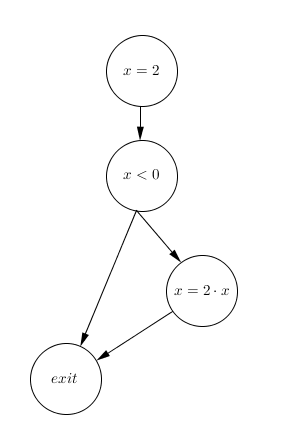
\includegraphics[scale=0.6]{graphics/simpleExample.png}
\caption{Directed graph of the program \ref{simple:example}}
\end{figure}


In the execution of this program, it is not possible to execute line 3 just after line 1 skipping line 2. We need to go line by line, respecting the execution flow. 
This is represented by the variable \pc (\concept{Program\IS counter}). This variable indicates the line to execute next.

So the state of the program at the beginning is 
%
\[ \pc = 1\]
%
This formula give all the information we have of the execution state. 
We know the \pc\; and the state and value of all variables (there are no more variables than \pc).

Now we need to define the step. 
%
How can we represent the execution of a line.
%
We need to use \concept{post-state} variables. 
%
We define the prime version of any variable to refer that same variable after the execution of the line (transition). 
%
Going back to the example, we have:
%
\[
\pc = 1 \andcond \pc'=2 \andcond x'=2 
\]

We have a post-state program counter ($\pc'=2$) and some post-state variables. 
%
As the execution of the assignment the variable $x$ takes a value (independently of the value in the pre-state), then $x'=2$ (regardless what value $x$ had). 

The next step could be
\[
\pc = 2 \andcond x'=x \andcond 	\pc'=?
\]

Where ? depends on the validity of the \textit{if} condition. 

This steps we have illustrated are called transition relations.

\begin{defn}[Transition relation]
A transition relation is the formula that define the step from one state of the program to another.  
\end{defn}

With this simple example, we have shown what a program counter and what a transition relation are. Now we can define the possible instructions a program may have.\footnote{We have just took the set of instructions the programs we are going to proof have.}

\subsubsection{Possible instructions}
As we are going to work with programs used by more than one thread, we need one program counter for each thread executing. 
%
We parametrize the program counter. 
%
This is, defining the \textbf{program counter} as a \textbf{function} that given a thread, returns its program counter. 
%
We could have define as one variable per thread, but it would be equivalent. 

For this definitions we use the letter $T$ to refer a particular thread.

\begin{description}
\item [Assignments:]
		The transition relation for a variable assignment consists of the 
		update of the program counter for the running thread and the 
		corresponding modification to the variable being assigned.
%
			\[
			\begin{array}[t]{p{8em}@{\hspace{6em}}p{\longtablesize}}
				\hline
				Statement & Transition relation \\ \hline\hline
				$\begin{array}[t]{l@{\hspace{0.3em}}c@{\hspace{1em}}l}
					l_1 & : & \mathtt{v := 2} \\
					l_2 & : & \mathtt{\cdots}
				\end{array}$
				&
				$\begin{array}[t]{ll}
					 \pc(T) = l_1 \andcond
					 \pc'(T) = l_2 \andcond
					 \mathtt{v}' = 2
				 \end{array}$ \\ 
				 \hline
			\end{array}
			\]
%
	\item [Pointer access:]
		Structure fields are accessible through the pointer operator \pointsto.
%
		There are two possible scenarios for the use of pointers, depending on 
		whether the statement accesses or modifies a structure field.
%
		We present now the semantics for both cases.
%
		The first case corresponds to the access of a structure field through an 
		address pointer.
%
\[
\begin{array}[t]{p{8em}@{\hspace{6em}}p{\longtablesize}}
	\hline
	Statement & Transition relation \\ \hline\hline
	$\begin{array}[t]{l@{\hspace{0.3em}}c@{\hspace{1em}}l}
		\ell_1 & : & \mathtt{v := a \pointsto field} \\ \\
		\ell_2 & : & \mathtt{\cdots}
	\end{array}$
	&
	$\begin{array}[t]{ll}
		 \pc(T) = \ell_1 \andcond
		 \pc'(T) = \ell_2 \andcond \\
		 \mathtt{v}' = \heap[\mathtt{a}].\mathtt{field}
	 \end{array}$ \\
	 \hline
\end{array}
\]
%
		The second case corresponds to the modification of a structure field using 
		an address pointer.
%
		Note how, in the second case, all structures (except the one pointed by 
		$\mathtt{b}$) remain unchanged.
%
		Also, all fields of the structure pointed by $\mathtt{b}$ remain unmodified 
		except for $\mathtt{field_n}$.
%
		\[
		\begin{array}[t]{p{8em}@{\hspace{6em}}p{\longtablesize}}
						\hline
						Statement & Transition relation \\ \hline\hline
						$\begin{array}[t]{l@{\hspace{0.3em}}c@{\hspace{1em}}l}
							\ell_1 & : & \mathtt{b \pointsto field_n := a} \\ \\ \\ \\
							\ell_2 & : & \mathtt{\cdots}
						\end{array}$
						&
						$\begin{array}[t]{ll}
							\pc(T) = \ell_1 \andcond \pc'(T) = \ell_2 & \andcond \\
							\heap' = \heap \{ \mathtt{b} \leftarrow c \} & \andcond \\
							c.\mathtt{field_n} = \mathtt{a} & \andcond \\
							\bigwedge\limits_{i \neq \mathtt{n}} c.\mathtt{field}_i = 
							\heap[\mathtt{b}].\mathtt{field}_i
						\end{array}$\\ \hline
			\end{array}
		\]

	\item [Conditionals:]
		We present now the two possible kinds of conditional statements in 
		SPL.
%
		In the first case, if condition $c$ does not hold, the execution 
		proceeds from the statement following the end of the conditional.
%
		\[
        \begin{array}[t]{p{8em}@{\hspace{6em}}p{\longtablesize}}
				\hline
				Statement & Transition relation \\ \hline\hline
				$\begin{array}[t]{l@{\hspace{0.3em}}c@{\hspace{1em}}l}
					\ell_1 & : & \mathtt{\textbf{if } c \textbf{ then }} \\ \\
					\ell_2 & : & \mathtt{\cdots} \\
						&& \mathtt{\vdots} \\
					\ell_n & : & \mathtt{\textbf{end if}} \\
					\ell_{n+1} & : & \mathtt{\cdots}
				\end{array}$
				&
				$\begin{array}[t]{ll}
					(\pc(T) = \ell_1 \andcond \;\;\mathtt{c} \andcond \pc'(T) = \ell_2) \; \Or \\
					(\pc(T) = \ell_1 \andcond \lnot \mathtt{c} \andcond \pc'(T) = \ell_{n+1})
				 \end{array}$ \\ \hline
			 \end{array}
		 \]
%
		In the second case, if condition $c$ does not hold, the execution 
		continues at the first statement in the \textbf{else} section of the 
		conditional statement.
%
		\[
				\begin{array}[t]{p{8em}@{\hspace{6em}}p{\longtablesize}}
				\hline
				Statement & Transition relation \\ \hline\hline
				$\begin{array}[t]{l@{\hspace{0.3em}}c@{\hspace{1em}}l}
					\ell_1 & : & \mathtt{\textbf{if } c \textbf{ then }} \\ \\
					\ell_2 & : & \mathtt{\cdots} \\
					\mathtt{\vdots} \\
					\ell_n & : & \mathtt{\textbf{else}} \\
					\ell_{n+1} & : & \mathtt{\cdots} \\
					\mathtt{\vdots} \\
					\ell_m & : & \mathtt{\textbf{end if}} \\
					\ell_{m+1} & : & \mathtt{\cdots}
				\end{array}$
				&
				$\begin{array}[t]{ll}
					(\pc(T) = \ell_1 \andcond \;\;\mathtt{c} \andcond \pc'(T) = \ell_2) \; \Or \\
					(\pc(T) = \ell_1 \andcond \lnot \mathtt{c} \andcond \pc'(T) = \ell_{n+1})
						& \text{for line } \ell_1 \\ \\ \phantom{\vdots} \\

						\pc(T) = \ell_n \andcond \pc'(T) = \ell_{m+1} & \text{for line } \ell_n
				 \end{array}$ \\ \hline
			\end{array}
		\]
%
	\item [Loops:]
		We consider the only loop statement available in SPL which executes 
	the statements in the body as long as the loop condition holds.
%
		\[
				\begin{array}[t]{p{8em}@{\hspace{6em}}p{\longtablesize}}
				\hline
				Statement & Transition relation \\ \hline\hline
				$\begin{array}[t]{l@{\hspace{0.3em}}c@{\hspace{1em}}l}
					\ell_1 & : & \mathtt{\textbf{while } c \textbf{ do }} \\
					\ell_2 & : & \mathtt{\cdots} \\
					\mathtt{\vdots} \\
					\ell_n & : & \mathtt{\textbf{end while}} \\
					\ell_{n+1} & : & \mathtt{\cdots}
				\end{array}$
				&
				$\begin{array}[t]{ll}
						(\pc(T) = \ell_1 \andcond \;\;\texttt{c} \andcond \pc'(T) = \ell_2) \; 
						\Or \\
						(\pc(T) = \ell_1 \andcond \lnot \texttt{c} \andcond \pc'(T) = 
					\ell_{n+1})
					& \text{for line $\ell_1$} \\ \\
					\pc(T) = \ell_n \andcond \pc'(T) = \ell_1 &
						\text{for line $\ell_n$}
				 \end{array}$ \\ \hline
			 \end{array}
		\]
%
			\item [Non deterministic choice:]
		The transition relation for the non-deterministic choice statement can 
		be expressed as follows:
%
		\[
			\begin{array}[t]{p{8em}@{\hspace{6em}}p{\longtablesize}}
				\hline
				Statement & Transition relation \\ \hline\hline
				$\begin{array}[t]{l@{\hspace{0.3em}}c@{\hspace{1em}}l}
					\ell_1 & : & \mathtt{\Nondet} \\
					\ell_2 & : & \mathtt{\;\;\;\;\;\; \cdots} \\
					\ell_3 & : & \mathtt{\textbf{or } \; \cdots} \\
					\mathtt{\vdots} \\
					\ell_n & : & \mathtt{\textbf{or } \; \cdots} \\
					\ell_{n+1} & : & \mathtt{\NondetEnd} \\
				\end{array}$
				&
				$\begin{array}[t]{ll}
					\pc(T) = \ell_1 \andcond
					\bigvee\limits_{i = 2..n} \pc'(T) = \ell_i
				 \end{array}$ \\ \hline
			 \end{array}
		\]
%
	\item [Lock and unlock:]
	Even though these are not SPL statements, as they will be widely used, it is necessary to define theirs transition relations.
%
		\[
			\begin{array}[t]{p{8em}@{\hspace{6em}}p{\longtablesize}}
				\hline
				Statement & Transition relation \\ \hline\hline
				$\begin{array}[t]{l@{\hspace{0.3em}}c@{\hspace{1em}}l}
					\ell_1 & : & \mathtt{\fLock(l)} \\
					\ell_2 & : & \mathtt{\cdots}
				\end{array}$
				&
				$\begin{array}[t]{ll}
					\pc(T) = \ell_1 \andcond
						\mathtt{l} = \oslash \andcond
						\mathtt{l}' = T \andcond \pc'(T) = \ell_2
				 \end{array}$ \\ \hline\hline
				$\begin{array}[t]{l@{\hspace{0.3em}}c@{\hspace{1em}}l}
					\ell_1 & : & \mathtt{\fUnlock(l)} \\
					\ell_2 & : & \mathtt{\cdots}
				\end{array}$
				&
				$\begin{array}[t]{ll}
					\pc(T) = \ell_1 \andcond
						\mathtt{l}' = \oslash \andcond \pc'(T) = \ell_2
				 \end{array}$ \\ \hline
			 \end{array}
		\]
%
\end{description}


% TODO: Mention the assume.
\subsection{Partial correctness (Safety)}

A function (or the whole program) is \textbf{partially correct} if when the function's precondition is satisfied on entry, its postcondition is satisfied when the function returns (if it ever does).
%
We present the \textbf{inductive assertion method} for proving partial correctness.


Let $\tau$ be the \gls{FOL} property to study. 
%
The procedure is the following:
%
First each function is reduced to a finite set of \gls{FOL} formulae called \concept[Verification condition]{\gls{VC}}.
%
\footnote{This reduction is done with the basic reducing cases we studied in \ref{def:SPL}.}
%
We achieve to prove that $\tau$ is valid in every state of the execution.
%
\textbf{Induction} is the methodology used.
%
First, we assert $\tau$ is valid before the program starts (induction base).
%
Then, we assume $\tau$ in the precondition and prove $\tau'$ valid.



Some examples are studied next to clarify the procedure.

\begin{example}



We study the loop version of the factorial function.


\[
	\begin{array}{l@{\hspace{0.3em}}c@{\hspace{1em}}l}
	\hline
		l_1 & : & \mathtt{x := 10} \\
		l_2 & : & \mathtt{f := 1} \\
		l_3 & : & \mathtt{\textbf{while } (x\geq 1) \textbf{ do }} \\
		l_4 & : & \mathtt{\;\;f = f*x} \\
		l_5 & : & \mathtt{\;\;x=x-1} \\ 	
		l_6 & : & \mathtt{\textbf{end while}}\\
		l_7 & : & \mathtt{\cdots}\\
	\hline
	\end{array}
\]
\label{simple:example}




We achieve to proof two formulae.

\[\tau_1 \equiv (l_5 \to \mathtt{x}\geq 1) \;\; \wedge \;\; \tau_2 \equiv \mathtt{x} \geq 0\]

First, we reduce the program to its \VC.


\[
	\begin{array}{l}
		 \psi_1 \equiv\pc(T) = l_1 \andcond \pc\prime (T) = l_2 \andcond \mathtt{f\prime =f} \andcond \mathtt{x}\prime  = 10\\
		 \psi_2 \equiv\pc(T) = l_2 \andcond \pc\prime (T) = l_3 \andcond \mathtt{f}\prime  = 1 \andcond x\prime =x\\
		 \psi_3 \equiv\pc(T) = l_3 \andcond \pc\prime (T) = l_4 \andcond \mathtt{f\prime =f} \andcond x\prime \geq 1\\
		 \psi_4 \equiv\pc(T) = l_4 \andcond \pc\prime (T) = l_5 \andcond \mathtt{f}\prime  = \mathtt{f*x} \andcond \mathtt{x\prime =x}\\
		 \psi_5 \equiv\pc(T) = l_5 \andcond \pc\prime (T) = l_3 \andcond \mathtt{f\prime =f} \andcond \mathtt{x\prime =x-1}\\
		 \psi_6 \equiv\pc(T) = l_3 \andcond \pc\prime (T) = l_7 \andcond \mathtt{f\prime =f} \andcond \mathtt{x<1}
	\end{array}
\]

We need to prove, for $i=1,2$:

\[
	\left\{
		\begin{array}{lr}
			\psi_1 \andcond \tau_i \to \tau_i\prime  &
			\psi_2 \andcond \tau_i \to \tau_i\prime \\
			\psi_3 \andcond \tau_i \to \tau_i\prime  &
			\psi_4 \andcond \tau_i \to \tau_i\prime \\
			\psi_5 \andcond \tau_i \to \tau_i\prime  &
			\psi_6 \andcond \tau_i \to \tau_i\prime 
		\end{array}
	\right.
\]

\begin{center}\rule{4cm}{0.4pt}  $\tau_1$  \rule{4cm}{0.4pt}\end{center}
	
	 $\psi_1 \andcond \tau_1 \to \tau_1\prime $:
%	\begin{dmath*}[indentstep={0em}]
	\begin{equation*}
		(
			\underbrace{\pc(T) = l_1 \andcond \pc\prime (T) = l_2 \andcond \mathtt{f\prime =f} \andcond \mathtt{x}\prime  = 10}_{\psi_1} \andcond (\underbrace{\pc(T) = l_5 \to \mathtt{x}\geq 1}_{\tau_1})
		) 
				\to(\underbrace{\pc\prime (T) = l_5 \to \mathtt{x}\prime  \geq 1}_{\tau_1\prime })\\\\
	\end{equation*}
%	\end{dmath*}


	The formula is valid because $\pc(T) = l_2 \neq l_5$ thus the $\tau\prime _1$ is true.

	 $\psi_2 \andcond \tau_1 \to \tau_1\prime $:
%	\begin{dmath*}[indentstep={0em}]
	\begin{equation*}
		(
			\underbrace{\pc(T) = l_2 \andcond \pc\prime (T) = l_3 \andcond \mathtt{f}\prime  = 1 \andcond x\prime =x}_{\psi_2} \andcond (\underbrace{\pc(T) = l_5 \to \mathtt{x}\geq 1}_{\tau_1})
		) 
			\to(\underbrace{\pc\prime (T) = l_5 \to \mathtt{x}\prime  \geq 1}_{\tau_1\prime })\\\\
	\end{equation*}
%	\end{dmath*}


	The formula is valid because $\pc(T) = l_3 \neq l_5$ thus the $\tau\prime _1$ is true.

	 $\psi_3 \andcond \tau_1 \to \tau_1\prime $:
%	\begin{dmath*}[indentstep={0em}]
	\begin{equation*}
		(
			\underbrace{\pc(T) = l_3 \andcond \pc\prime (T) = l_4 \andcond \mathtt{f\prime =f} \andcond x\prime \geq 1}_{\psi_3} \andcond (\underbrace{\pc(T) = l_5 \to \mathtt{x}\geq 1}_{\tau_1})
		) 
			\to(\underbrace{\pc\prime (T) = l_5 \to \mathtt{x}\prime  \geq 1}_{\tau_1\prime })\\\\
	\end{equation*}
%	\end{dmath*}

		The formula is valid because $\pc(T) = l_4 \neq l_5$ thus the $\tau\prime _1$ is true.

	 \;$\psi_4 \andcond \tau_1 \to \tau_1\prime $: 
%	\begin{dmath*}[indentstep={0em}]
	\begin{equation*}
		(
			\underbrace{\pc(T) = l_4 \andcond \pc\prime (T) = l_5 \andcond \mathtt{f}\prime  = \mathtt{f*x} \andcond \mathtt{x\prime =x}}_{\psi_4} \andcond (\underbrace{\pc(T) = l_5 \to \mathtt{x}\geq 1}_{\tau_1})
		) 
			\to(\underbrace{\pc\prime (T) = l_5 \to \mathtt{x}\prime  \geq 1}_{\tau_1\prime })\\\\
	\end{equation*}
%	\end{dmath*}

	The formula is equivalent (applying resolution) to

%	\begin{dmath*}[indentstep={0em}]
	\begin{equation*}
		(
			\mathtt{x\prime =x} \andcond  \mathtt{x}\geq 1
		) 
		\to (\mathtt{x}\prime \geq 1)
	\end{equation*}
%	\end{dmath*}


	Which is valid because of equality congruence.

	 $\psi_5 \andcond \tau_1 \to \tau_1\prime $:
%	\begin{dmath*}[indentstep={0em}]
	\begin{equation*}
		(
			\underbrace{\pc(T) = l_5 \andcond \pc\prime (T) = l_3 \andcond \mathtt{f\prime =f} \andcond \mathtt{x\prime =x-1}}_{\psi_5} \andcond (\underbrace{\pc(T) = l_5 \to \mathtt{x}\geq 1}_{\tau_1})
		) 
			\to(\underbrace{\pc\prime (T) = l_5 \to \mathtt{x}\prime  \geq 1}_{\tau_1\prime })\\\\
	\end{equation*}
%	\end{dmath*}


	The formula is valid because $\pc(T) = l_3 \neq l_5$ thus the $\tau\prime _1$ is true.

	 $\psi_6 \andcond \tau_1 \to \tau_1\prime $:
%	\begin{dmath*}[indentstep={0em}]
	\begin{equation*}
		(
			\underbrace{\pc(T) = l_3 \andcond \pc\prime (T) = l_7 \andcond \mathtt{f\prime =f} \andcond \mathtt{x<1}}_{\psi_6} \andcond \underbrace{\pc(T) = l_5 \to \mathtt{x} \geq 1}_{\tau_1}
		) 
			\to (\underbrace{\pc\prime (T) = l_5 \to \mathtt{x}\prime  \geq 1}_{\tau_1\prime })\\\\
	\end{equation*}
%	\end{dmath*}


	The formula is valid because $\pc(T) = l_7 \neq l_5$ thus the $\tau\prime _1$ is true.


\paragraph{Conclusion:} we have proven that $\pc(T) = l_5 \to x \geq 1$. 
%
This is called an \concept[Invariant]{invariant} because it is true during all the execution. 
%
This transition has been chosen specially because it is needed in the proof of $\tau_2$.

\begin{center}\rule{4cm}{0.4pt}  $\tau_2$  \rule{4cm}{0.4pt}\end{center}

	\; $\psi_1 \andcond \tau_2 \to \tau_2\prime $:	
%	\begin{dmath*}[indentstep={0em}]
	\begin{equation*}
		(
			\underbrace{\pc(T) = l_1 \andcond \pc\prime (T) = l_2 \andcond \mathtt{f\prime =f} \andcond \mathtt{x}\prime  = 10}_{\psi_1} \andcond \underbrace{\mathtt{x} \geq 0}_{\tau_2}
		) 
				\to  \underbrace{\mathtt{x}\prime  \geq 0}_{\tau_2\prime }\\\\
	\end{equation*}
%	\end{dmath*}


	The formula is valid because $x\prime =10 \to x\prime \geq 0$.

	\; $\psi_2 \andcond \tau_2 \to \tau_2\prime $:	
%	\begin{dmath*}[indentstep={0em}]
	\begin{equation*}
		(
			\underbrace{\pc(T) = l_2 \andcond \pc\prime (T) = l_3 \andcond \mathtt{f}\prime  = 1 \andcond x\prime =x}_{\psi_2} \andcond \underbrace{\mathtt{x} \geq 0}_{\tau_2}
		) 
			\to \underbrace{\mathtt{x}\prime  \geq 0}_{\tau_2\prime }\\\\
	\end{equation*}
%	\end{dmath*}



	The formula is valid because of the congruence of equality used in  $x\prime =x \andcond x\geq 0 \to x\prime \geq 0$ 

	\; $\psi_3 \andcond \tau_2 \to \tau_2\prime $:
%	\begin{dmath*}[indentstep={0em}]
	\begin{equation*}
		(
			\underbrace{\pc(T) = l_3 \andcond \pc\prime (T) = l_4 \andcond \mathtt{f\prime =f} \andcond x\prime \geq 1}_{\psi_3} \andcond \underbrace{\mathtt{x} \geq 0}_{\tau_2}
		) 
			\to \underbrace{\mathtt{x}\prime  \geq 0}_{\tau_2\prime }\\\\
	\end{equation*}
%	\end{dmath*}


	The formula is valid because $x\prime \geq 1 \to x\prime \geq 0$.
	\; $\psi_4 \andcond \tau_2 \to \tau_2\prime $:	
%	\begin{dmath*}[indentstep={0em}]
	\begin{equation*}
		(
			\underbrace{\pc(T) = l_4 \andcond \pc\prime (T) = l_5 \andcond \mathtt{f}\prime  = \mathtt{f*x} \andcond \mathtt{x\prime =x}}_{\psi_4} \andcond \underbrace{\mathtt{x} \geq 0}_{\tau_2}
		) 
			\to \underbrace{\mathtt{x}\prime  \geq 0}_{\tau_2\prime }\\\\
	\end{equation*}
%	\end{dmath*}


	The formula is valid because of the congruence of equality used in  $x\prime =x \andcond x\geq 0 \to x\prime \geq 0$ 

	\; $\psi_5 \andcond \tau_2 \to \tau_2\prime $:	
%	\begin{dmath*}[indentstep={0em}]
	\begin{equation*}
		(
			\underbrace{\pc(T) = l_5 \andcond \pc\prime (T) = l_3 \andcond \mathtt{f\prime =f} \andcond \mathtt{x\prime =x-1}}_{\psi_5} \andcond \underbrace{\mathtt{x} \geq 0}_{\tau_2}
		) 
			\to \underbrace{\mathtt{x}\prime  \geq 0}_{\tau_2\prime }\\\\
	\end{equation*}
%	\end{dmath*}


	The formula has some more difficulty. 
	%
	Inside the loop $x$ should be greater than 1.
	%
	However, that information is not in the implication to prove.
	
	The solution is use some \concept{support}.
	%
	A support formula is a formula added to the precedent of an implication to give more information. 
	%
	This addition does not change the validity of the formula.
	%
	We could equivalently prove

	\[
		(\psi_5 \andcond \tau_1 \andcond \tau_2 \to \tau_2\prime ) rightarrow (\psi_5\andcond \tau_2\to\tau_2\prime )
	\]

	And this is exactly the solution to proof this \gls{VC}

	

%	\begin{dmath*}[indentstep={0em}]
	\begin{equation*}
		(
			\underbrace{\pc(T) = l_5 \andcond \pc\prime (T) = l_3 \andcond \mathtt{f\prime =f} \andcond \mathtt{x\prime =x-1}}_{\psi_5} \andcond \underbrace{\mathtt{x} \geq 0}_{\tau_2} \andcond \underbrace{\pc(T) = l_5 \to \mathtt{x} \geq 1}_{\tau_1}
		) 
			\to \underbrace{\mathtt{x}\prime  \geq 0}_{\tau_2\prime }\\\\
	\end{equation*}
%	\end{dmath*}


	And this formula is valid. Applying resolution we get an equivalent valid formula:

	\[
		( \mathtt{x\prime =x-1} \andcond \mathtt{x\prime }\geq 1) \to \mathtt{x} \geq 0
	\]


	\; $\psi_6 \andcond \tau_2 \to \tau_2\prime $:
%	\begin{dmath*}[indentstep={0em}]
	\begin{equation*}
		(
			\underbrace{\pc(T) = l_3 \andcond \pc\prime (T) = l_7 \andcond \mathtt{f\prime =f} \andcond \mathtt{x<1} \andcond \mathtt{x\prime =x} }_{\psi_6} \andcond \underbrace{\mathtt{x} \geq 0}_{\tau_2}
		) 
			\to \underbrace{\mathtt{x}\prime  \geq 0}_{\tau_2\prime }\\\\
	\end{equation*}
%	\end{dmath*}


	The formula has some more difficulty too.
	%
	One can think that the unique possible value of $x$ should be $0$ because of the content of the loop.
	%
	However, that information is not within the formula.
	%
	As we did before, some support is needed to prove this formula.
	%
	The support needed is $\tau_3 \equiv \pc(T) = l_3 \to \mathtt{x} \geq 0$.
	%
	The proof of this invariant is not included because it does not give new relevant information. 
	%
	Using this invariant, we have:

	

%	\begin{dmath*}[indentstep={0em}]
	\begin{equation*}
		(
			\underbrace{\pc(T) = l_3 \andcond \pc\prime (T) = l_7 \andcond \mathtt{f\prime =f} \andcond \mathtt{x<1} \andcond \mathtt{x\prime =x}}_{\psi_6} \andcond \underbrace{\mathtt{x} \geq 0}_{\tau_2} \andcond \underbrace{\pc(T) = l_3 \to \mathtt{x}\geq 0 }_{\tau_3}
		) 
			\to \underbrace{\mathtt{x}\prime  \geq 0}_{\tau_2\prime }\\\\
	\end{equation*}
%	\end{dmath*}

	
	And this formula is valid. Applying resolution we get an equivalent valid formula:

	\[
		(
			\mathtt{x\prime =x}  \andcond \mathtt{x}\geq 0 \to \mathtt{x\prime }\geq 0
		)
	\]



\end{example}



\subsection{Total correctness (Lifeness)}

\todo{Complete with Césars Book}
What is proving lifeness, for what we need temporal logic.

\subsubsection{Temporal logic}

Basics on temporal logics

Temporal logic studies problems like the one exposed below.

\begin{example}
\label{Collatz:conjecture}

Let $f$ be the following function.

\[
f(n) = \left\{
	\begin{array}{cc}
		\rfrac{n}{2} & \text{ if } (n\text{ mod } 2) \equiv 0\\
		3n+1 & \text{ if } (n\text{ mod } 2) \equiv 1
	\end{array}
\right.
\]

We can form a sequence applying repeatedly $f$. If we take the sequence starting in $n=13$ we get:

\[ 
	13 \overset{\displaystyle\;\; 3n+1\;\;}{\longrightarrow}
	40 \overset{\displaystyle\;\;\rfrac{n}{2}\;\;}{\longrightarrow}
	20 \overset{\displaystyle\;\;\rfrac{n}{2}\;\;}{\longrightarrow}
	10 \overset{\displaystyle\;\;\rfrac{n}{2}\;\;}{\longrightarrow}
	5 \overset{\displaystyle\;\; 3n+1\;\;}{\longrightarrow}
	16 \overset{\displaystyle\;\;\rfrac{n}{2}\;\;}{\longrightarrow}
	8 \overset{\displaystyle\;\;\rfrac{n}{2}\;\;}{\longrightarrow}
	4 \overset{\displaystyle\;\;\rfrac{n}{2}\;\;}{\longrightarrow}
	2 \overset{\displaystyle\;\;\rfrac{n}{2}\;\;}{\longrightarrow}
	1
\]

One could ask if this sequence eventually stops regardless the integer chosen to begin. This question is called \concept{Collatz conjecture} and has not been solved yet. 
For the moment, an infinite sequence has not been found, but the temporal logic problem has not been proven either.

The temporal formula for this problem is:

\todo{Formula of conjecture}


\end{example}


\subsection{Parametrized systems}

The correctness of just one thread executing a program it is an easy problem because it runs sequentiality.
%
Multiple threads executing the same program is a different and more difficult problem to solve.
%
If the number of threads executing is not bounded is another important and difficult step.
%
If the number of threads is bound, one could unroll the formula for all the threads in the problem and try to prove it. 
%
This is why we focus the unbounded case, which is the usual scenario.

We are going to study those cases. 
%
To do so, we need to parametrize the program executed by multiple threads.
%
Typically the threads would be $i$,$j$,$k_0$,$k_1$,... 



\subsubsection{Arbitrary number of threads}


For example, the web servers may not have a bound of the number of clients they can accept.
%
Can we prove correctness when an unbounded number of processes are using the same global variabless?

A recent research \citeapos{paperParametrizedInvariants} has proven a very important result. 
%
We will enunciate it and discuss it because it is fundamental for this work. 
%
We will not prove any of the results proven in \citep{paperParametrizedInvariants}.

Before we enunciate the theorem, we need some previous concepts.
%
We need to extend the concept of support to parametrized formulas.


\begin{defn}[Support]
  Let $\psi$, $A$ and $B$ be parametrized formulas, and let $S$ be the
  set of possible substitutions from the set of parametrized variables in $\psi$ ($\Var(\psi)$) into the set of parametrized variables of $(A\Into B)$ ($\Var(A\Into B)$).
%
  We say that $\psi$ supports $(A\Into B)$, whenever
%
  \[ \big( (\bigwedge_{\sigma\in S} \sigma(\psi)\big) \andcond A\big) \Into B \hspace{4em} \text{is valid} \]
%
  We use $\psi\supports(A\Into B)$ as a short notation for
  $\big((\bigwedge_{\sigma\in S} \sigma(\psi)) \andcond A\big) \Into B$.  
\end{defn}

Note that if $S'\subseteq S$ is a subset of the substitutions, and 
%
  \[ \big( (\bigwedge_{\sigma\in S'} \sigma(\psi)\big) \andcond A\big) \Into B \hspace{4em} \text{is valid} \]
%
then
%
  \[ \big( (\bigwedge_{\sigma\in S} \sigma(\psi)\big) \andcond A\big) \Into B \hspace{4em} \text{is also valid} \]
%
  Essentially, if one is successful proving the validity of a formula obtained by removing some of the conjuncts from the antecedent, the validity of the full formula holds.
%
  Hence, in practice, it is enough to consider only some of the partial substitutions to show that a support formula is valid.


\begin{itheorem}[Bound an arbitrary number of threads]
	Let $\varphi$ be a thread-parametrized formula, where $\overline{k}=\Var(\varphi)$. 
	%
	Let $\tau$ be a transition of $P$ and $\ThetaParam$ the initial condition.

	To show that $P$ satisfies $\Always\varphi$:
	\hspace{-1em}
	\[ 
		\begin{array}{r@{\;\;}lr@{\;}@{\;}cl@{\hspace{1em}}l}
			\Premise{S1}. & & \ThetaParam(\overline{k}) &\supports & \varphi & \\

			\Premise{S2}. & \varphi \supports & \tau^{(i)} &\Into& \varphi'  & \text{forall $\tau$ and all $i\in \overline{k}$}\\
			\Premise{S3}. & \varphi\supports & \big(\bigwedge\limits_{x\in\Var(\varphi)} j\neq x \andcond \tau^{(j)} &\Into& \varphi' \big)& \text{forall $\tau$ and one fresh $j\notin\overline{k}$}\\ \hline
			& \multicolumn{4}{c}{\hspace{3em} \Always \varphi} &
		\end{array}
	\]
\label{thm:biggest}
\end{itheorem}


Using this powerful result, we have reduced an arbitrary number of processes sharing the same variables to a finite number of threads sharing the variable. 
%
We will refer to $\Premise{S1}$ as \textit{initiation}, to $\Premise{S2}$ self-consecution and to $\Premise{S3}$ others-consecution. 
%

\begin{example}
\todo{example}
\end{example}



%
% Diseño
%
% -*- root: ../main.tex -*-
\chapter{Design\label{chap:design}}

\paragraph{Abstract} 
%In this chapter we cover the description of the theory used. As we mentioned before is the linked list theory, but one may implement this theory in many different ways. 

%Once the theory we are working with is defined, we will expose the goals we intend to prove and which are the intermediate steps to prove the safety of this theory.


\section{Program correctness}


We are finally ready to apply this concepts to a real word problem. In this \thisworkm we apply those concepts to prove some properties of programs.
%
The remaining task is to define the framework and the conventions we use to prove formally properties of programs.

The way of proving correctness is by proving properties. 
%
There are \concept{liveness}, \concept{safety} and \concept{functional} properties. 
%
Safety properties refer, informally, to "bad things never happens". Proving \textit{ variable x is never 0 } is a safety property. 
%
Proving its validity can assure that a division by zero error does never occur. 
%
Whether a program finishes or not is a liveness property and receiving an output for a concrete input is a functional property. 

This properties are written in some logic. Liveness properties need \gls{LTL} but \gls{FOL} is enough to prove safety properties. 
%
As the properties are expressed formally in logic, it is necessary to define a formal representation of a program.


\label{def:SPL}
% -*- root: ../main.tex -*-
\subsection{Formal representation of a program}

This \gls{SPL} and its formal representation is the language chosen to write the programs to be formally verified.
%
It has been chosen by \citep{thesisAle} because its simplicity and \doubt{expressiveness} in order to write concurrent programs. 
%
Because its simplicity it is a great option to do formal verification with it.


\subsubsection{Preliminaries (Notation, definition)}

One can consider a program as a series of state changes. There are some variables, we execute one line of the program and some of those variables changes and some others don't. Thus, we can consider any program as a graph of states with some ways. For example, lets take a very simple program:
%
\[
	\begin{array}{l@{\hspace{0.3em}}c@{\hspace{1em}}l}
	\hline
		l_1 & : & \mathtt{x := -2} \\
		l_2 & : & \mathtt{\textbf{if } (x<0)} \\
		l_3 & : & \mathtt{\;\;x = 2x} \\
		l_4 & : & \mathtt{\textbf{...}}\\
	\hline
	\end{array}
\]
\label{simple:example}

This simple program doesn't do anything interesting, but it is useful to illustrate.
%
In figure \ref{ex:simpleExample} the directed graph of states is shown.

\begin{figure}[hbtp]
\label{ex:simpleExample}
\centering
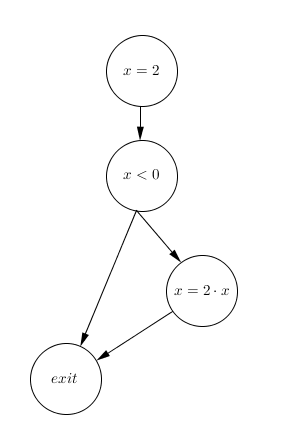
\includegraphics[scale=0.6]{graphics/simpleExample.png}
\caption{Directed graph of the program \ref{simple:example}}
\end{figure}


In the execution of this program, it is not possible to execute line 3 just after line 1 skipping line 2. We need to go line by line, respecting the execution flow. 
This is represented by the variable \pc (\concept{Program\IS counter}). This variable indicates the line to execute next.

So the state of the program at the beginning is 
%
\[ \pc = 1\]
%
This formula give all the information we have of the execution state. 
We know the \pc\; and the state and value of all variables (there are no more variables than \pc).

Now we need to define the step. 
%
How can we represent the execution of a line.
%
We need to use \concept{post-state} variables. 
%
We define the prime version of any variable to refer that same variable after the execution of the line (transition). 
%
Going back to the example, we have:
%
\[
\pc = 1 \andcond \pc'=2 \andcond x'=2 
\]

We have a post-state program counter ($\pc'=2$) and some post-state variables. 
%
As the execution of the assignment the variable $x$ takes a value (independently of the value in the pre-state), then $x'=2$ (regardless what value $x$ had). 

The next step could be
\[
\pc = 2 \andcond x'=x \andcond 	\pc'=?
\]

Where ? depends on the validity of the \textit{if} condition. 

This steps we have illustrated are called transition relations.

\begin{defn}[Transition relation]
A transition relation is the formula that define the step from one state of the program to another.  
\end{defn}

With this simple example, we have shown what a program counter and what a transition relation are. Now we can define the possible instructions a program may have.\footnote{We have just took the set of instructions the programs we are going to proof have.}

\subsubsection{Possible instructions}
As we are going to work with programs used by more than one thread, we need one program counter for each thread executing. 
%
We parametrize the program counter. 
%
This is, defining the \textbf{program counter} as a \textbf{function} that given a thread, returns its program counter. 
%
We could have define as one variable per thread, but it would be equivalent. 

For this definitions we use the letter $T$ to refer a particular thread.

\begin{description}
\item [Assignments:]
		The transition relation for a variable assignment consists of the 
		update of the program counter for the running thread and the 
		corresponding modification to the variable being assigned.
%
			\[
			\begin{array}[t]{p{8em}@{\hspace{6em}}p{\longtablesize}}
				\hline
				Statement & Transition relation \\ \hline\hline
				$\begin{array}[t]{l@{\hspace{0.3em}}c@{\hspace{1em}}l}
					l_1 & : & \mathtt{v := 2} \\
					l_2 & : & \mathtt{\cdots}
				\end{array}$
				&
				$\begin{array}[t]{ll}
					 \pc(T) = l_1 \andcond
					 \pc'(T) = l_2 \andcond
					 \mathtt{v}' = 2
				 \end{array}$ \\ 
				 \hline
			\end{array}
			\]
%
	\item [Pointer access:]
		Structure fields are accessible through the pointer operator \pointsto.
%
		There are two possible scenarios for the use of pointers, depending on 
		whether the statement accesses or modifies a structure field.
%
		We present now the semantics for both cases.
%
		The first case corresponds to the access of a structure field through an 
		address pointer.
%
\[
\begin{array}[t]{p{8em}@{\hspace{6em}}p{\longtablesize}}
	\hline
	Statement & Transition relation \\ \hline\hline
	$\begin{array}[t]{l@{\hspace{0.3em}}c@{\hspace{1em}}l}
		\ell_1 & : & \mathtt{v := a \pointsto field} \\ \\
		\ell_2 & : & \mathtt{\cdots}
	\end{array}$
	&
	$\begin{array}[t]{ll}
		 \pc(T) = \ell_1 \andcond
		 \pc'(T) = \ell_2 \andcond \\
		 \mathtt{v}' = \heap[\mathtt{a}].\mathtt{field}
	 \end{array}$ \\
	 \hline
\end{array}
\]
%
		The second case corresponds to the modification of a structure field using 
		an address pointer.
%
		Note how, in the second case, all structures (except the one pointed by 
		$\mathtt{b}$) remain unchanged.
%
		Also, all fields of the structure pointed by $\mathtt{b}$ remain unmodified 
		except for $\mathtt{field_n}$.
%
		\[
		\begin{array}[t]{p{8em}@{\hspace{6em}}p{\longtablesize}}
						\hline
						Statement & Transition relation \\ \hline\hline
						$\begin{array}[t]{l@{\hspace{0.3em}}c@{\hspace{1em}}l}
							\ell_1 & : & \mathtt{b \pointsto field_n := a} \\ \\ \\ \\
							\ell_2 & : & \mathtt{\cdots}
						\end{array}$
						&
						$\begin{array}[t]{ll}
							\pc(T) = \ell_1 \andcond \pc'(T) = \ell_2 & \andcond \\
							\heap' = \heap \{ \mathtt{b} \leftarrow c \} & \andcond \\
							c.\mathtt{field_n} = \mathtt{a} & \andcond \\
							\bigwedge\limits_{i \neq \mathtt{n}} c.\mathtt{field}_i = 
							\heap[\mathtt{b}].\mathtt{field}_i
						\end{array}$\\ \hline
			\end{array}
		\]

	\item [Conditionals:]
		We present now the two possible kinds of conditional statements in 
		SPL.
%
		In the first case, if condition $c$ does not hold, the execution 
		proceeds from the statement following the end of the conditional.
%
		\[
        \begin{array}[t]{p{8em}@{\hspace{6em}}p{\longtablesize}}
				\hline
				Statement & Transition relation \\ \hline\hline
				$\begin{array}[t]{l@{\hspace{0.3em}}c@{\hspace{1em}}l}
					\ell_1 & : & \mathtt{\textbf{if } c \textbf{ then }} \\ \\
					\ell_2 & : & \mathtt{\cdots} \\
						&& \mathtt{\vdots} \\
					\ell_n & : & \mathtt{\textbf{end if}} \\
					\ell_{n+1} & : & \mathtt{\cdots}
				\end{array}$
				&
				$\begin{array}[t]{ll}
					(\pc(T) = \ell_1 \andcond \;\;\mathtt{c} \andcond \pc'(T) = \ell_2) \; \Or \\
					(\pc(T) = \ell_1 \andcond \lnot \mathtt{c} \andcond \pc'(T) = \ell_{n+1})
				 \end{array}$ \\ \hline
			 \end{array}
		 \]
%
		In the second case, if condition $c$ does not hold, the execution 
		continues at the first statement in the \textbf{else} section of the 
		conditional statement.
%
		\[
				\begin{array}[t]{p{8em}@{\hspace{6em}}p{\longtablesize}}
				\hline
				Statement & Transition relation \\ \hline\hline
				$\begin{array}[t]{l@{\hspace{0.3em}}c@{\hspace{1em}}l}
					\ell_1 & : & \mathtt{\textbf{if } c \textbf{ then }} \\ \\
					\ell_2 & : & \mathtt{\cdots} \\
					\mathtt{\vdots} \\
					\ell_n & : & \mathtt{\textbf{else}} \\
					\ell_{n+1} & : & \mathtt{\cdots} \\
					\mathtt{\vdots} \\
					\ell_m & : & \mathtt{\textbf{end if}} \\
					\ell_{m+1} & : & \mathtt{\cdots}
				\end{array}$
				&
				$\begin{array}[t]{ll}
					(\pc(T) = \ell_1 \andcond \;\;\mathtt{c} \andcond \pc'(T) = \ell_2) \; \Or \\
					(\pc(T) = \ell_1 \andcond \lnot \mathtt{c} \andcond \pc'(T) = \ell_{n+1})
						& \text{for line } \ell_1 \\ \\ \phantom{\vdots} \\

						\pc(T) = \ell_n \andcond \pc'(T) = \ell_{m+1} & \text{for line } \ell_n
				 \end{array}$ \\ \hline
			\end{array}
		\]
%
	\item [Loops:]
		We consider the only loop statement available in SPL which executes 
	the statements in the body as long as the loop condition holds.
%
		\[
				\begin{array}[t]{p{8em}@{\hspace{6em}}p{\longtablesize}}
				\hline
				Statement & Transition relation \\ \hline\hline
				$\begin{array}[t]{l@{\hspace{0.3em}}c@{\hspace{1em}}l}
					\ell_1 & : & \mathtt{\textbf{while } c \textbf{ do }} \\
					\ell_2 & : & \mathtt{\cdots} \\
					\mathtt{\vdots} \\
					\ell_n & : & \mathtt{\textbf{end while}} \\
					\ell_{n+1} & : & \mathtt{\cdots}
				\end{array}$
				&
				$\begin{array}[t]{ll}
						(\pc(T) = \ell_1 \andcond \;\;\texttt{c} \andcond \pc'(T) = \ell_2) \; 
						\Or \\
						(\pc(T) = \ell_1 \andcond \lnot \texttt{c} \andcond \pc'(T) = 
					\ell_{n+1})
					& \text{for line $\ell_1$} \\ \\
					\pc(T) = \ell_n \andcond \pc'(T) = \ell_1 &
						\text{for line $\ell_n$}
				 \end{array}$ \\ \hline
			 \end{array}
		\]
%
			\item [Non deterministic choice:]
		The transition relation for the non-deterministic choice statement can 
		be expressed as follows:
%
		\[
			\begin{array}[t]{p{8em}@{\hspace{6em}}p{\longtablesize}}
				\hline
				Statement & Transition relation \\ \hline\hline
				$\begin{array}[t]{l@{\hspace{0.3em}}c@{\hspace{1em}}l}
					\ell_1 & : & \mathtt{\Nondet} \\
					\ell_2 & : & \mathtt{\;\;\;\;\;\; \cdots} \\
					\ell_3 & : & \mathtt{\textbf{or } \; \cdots} \\
					\mathtt{\vdots} \\
					\ell_n & : & \mathtt{\textbf{or } \; \cdots} \\
					\ell_{n+1} & : & \mathtt{\NondetEnd} \\
				\end{array}$
				&
				$\begin{array}[t]{ll}
					\pc(T) = \ell_1 \andcond
					\bigvee\limits_{i = 2..n} \pc'(T) = \ell_i
				 \end{array}$ \\ \hline
			 \end{array}
		\]
%
	\item [Lock and unlock:]
	Even though these are not SPL statements, as they will be widely used, it is necessary to define theirs transition relations.
%
		\[
			\begin{array}[t]{p{8em}@{\hspace{6em}}p{\longtablesize}}
				\hline
				Statement & Transition relation \\ \hline\hline
				$\begin{array}[t]{l@{\hspace{0.3em}}c@{\hspace{1em}}l}
					\ell_1 & : & \mathtt{\fLock(l)} \\
					\ell_2 & : & \mathtt{\cdots}
				\end{array}$
				&
				$\begin{array}[t]{ll}
					\pc(T) = \ell_1 \andcond
						\mathtt{l} = \oslash \andcond
						\mathtt{l}' = T \andcond \pc'(T) = \ell_2
				 \end{array}$ \\ \hline\hline
				$\begin{array}[t]{l@{\hspace{0.3em}}c@{\hspace{1em}}l}
					\ell_1 & : & \mathtt{\fUnlock(l)} \\
					\ell_2 & : & \mathtt{\cdots}
				\end{array}$
				&
				$\begin{array}[t]{ll}
					\pc(T) = \ell_1 \andcond
						\mathtt{l}' = \oslash \andcond \pc'(T) = \ell_2
				 \end{array}$ \\ \hline
			 \end{array}
		\]
%
\end{description}



\subsection{Partial correctness (Safety)}

A function (or the whole program) is \textbf{partially correct} if when the function's precondition is satisfied on entry, its postcondition is satisfied when the function returns (if it ever does).
%
We present the \textbf{inductive assertion method} for proving partial correctness.


Let $\tau$ be the \gls{FOL} property to study. 
%
The procedure is the following:
%
First each function is reduced to a finite set of \gls{FOL} formulae called \concept[Verification condition]{\gls{VC}}.
%
This reduction is done with the basic reducing cases we studied in \ref{def:SPL}.
%
The goal is to prove that $\tau$ is valid in every state of the execution.
%
\textbf{Induction} is the methodology used.
%
First, we assert $\tau$ is valid before the program starts (induction base).
%
Then, we assume $\tau$ in the precondition and prove $\tau'$ valid (induction step) for every possible transition.


An example is presented to clarify the method.

\begin{example}



We study the loop version of the factorial function.


\[
	\begin{array}{l@{\hspace{0.3em}}c@{\hspace{1em}}l}
	\hline
		l_1 & : & \mathtt{x := 10} \\
		l_2 & : & \mathtt{f := 1} \\
		l_3 & : & \mathtt{\textbf{while } (x\geq 1) \textbf{ do }} \\
		l_4 & : & \mathtt{\;\;f = f*x} \\
		l_5 & : & \mathtt{\;\;x=x-1} \\ 	
		l_6 & : & \mathtt{\textbf{end while}}\\
		l_7 & : & \mathtt{\cdots}\\
	\hline
	\end{array}
\]
\label{simple:example}




We achieve to proof two formulae.

\[\tau_1 \equiv (l_5 \to \mathtt{x}\geq 1) \;\; \wedge \;\; \tau_2 \equiv \mathtt{x} \geq 0\]

First, we reduce the program to its \VC.


\[
	\begin{array}{l}
		 \psi_1 \equiv\pc(T) = l_1 \andcond \pc\prime (T) = l_2 \andcond \mathtt{f\prime =f} \andcond \mathtt{x}\prime  = 10\\
		 \psi_2 \equiv\pc(T) = l_2 \andcond \pc\prime (T) = l_3 \andcond \mathtt{f}\prime  = 1 \andcond x\prime =x\\
		 \psi_3 \equiv\pc(T) = l_3 \andcond \pc\prime (T) = l_4 \andcond \mathtt{f\prime =f} \andcond x\prime \geq 1\\
		 \psi_4 \equiv\pc(T) = l_4 \andcond \pc\prime (T) = l_5 \andcond \mathtt{f}\prime  = \mathtt{f*x} \andcond \mathtt{x\prime =x}\\
		 \psi_5 \equiv\pc(T) = l_5 \andcond \pc\prime (T) = l_3 \andcond \mathtt{f\prime =f} \andcond \mathtt{x\prime =x-1}\\
		 \psi_6 \equiv\pc(T) = l_3 \andcond \pc\prime (T) = l_7 \andcond \mathtt{f\prime =f} \andcond \mathtt{x<1}
	\end{array}
\]

We need to prove, for $i=1,2$:

\[
	\left\{
		\begin{array}{lr}
			\psi_1 \andcond \tau_i \to \tau_i\prime  &
			\psi_2 \andcond \tau_i \to \tau_i\prime \\
			\psi_3 \andcond \tau_i \to \tau_i\prime  &
			\psi_4 \andcond \tau_i \to \tau_i\prime \\
			\psi_5 \andcond \tau_i \to \tau_i\prime  &
			\psi_6 \andcond \tau_i \to \tau_i\prime 
		\end{array}
	\right.
\]

\begin{center}\rule{4cm}{0.4pt}  $\tau_1$  \rule{4cm}{0.4pt}\end{center}
	
	 $\psi_1 \andcond \tau_1 \to \tau_1\prime $:
%	\begin{dmath*}[indentstep={0em}]
	\begin{equation*}
		(
			\underbrace{\pc(T) = l_1 \andcond \pc\prime (T) = l_2 \andcond \mathtt{f\prime =f} \andcond \mathtt{x}\prime  = 10}_{\psi_1} \andcond (\underbrace{\pc(T) = l_5 \to \mathtt{x}\geq 1}_{\tau_1})
		) 
				\to(\underbrace{\pc\prime (T) = l_5 \to \mathtt{x}\prime  \geq 1}_{\tau_1\prime })\\\\
	\end{equation*}
%	\end{dmath*}


	The formula is valid because $\pc(T) = l_2 \neq l_5$ thus the $\tau\prime _1$ is true.

	 $\psi_2 \andcond \tau_1 \to \tau_1\prime $:
%	\begin{dmath*}[indentstep={0em}]
	\begin{equation*}
		(
			\underbrace{\pc(T) = l_2 \andcond \pc\prime (T) = l_3 \andcond \mathtt{f}\prime  = 1 \andcond x\prime =x}_{\psi_2} \andcond (\underbrace{\pc(T) = l_5 \to \mathtt{x}\geq 1}_{\tau_1})
		) 
			\to(\underbrace{\pc\prime (T) = l_5 \to \mathtt{x}\prime  \geq 1}_{\tau_1\prime })\\\\
	\end{equation*}
%	\end{dmath*}


	The formula is valid because $\pc(T) = l_3 \neq l_5$ thus the $\tau\prime _1$ is true.

	 $\psi_3 \andcond \tau_1 \to \tau_1\prime $:
%	\begin{dmath*}[indentstep={0em}]
	\begin{equation*}
		(
			\underbrace{\pc(T) = l_3 \andcond \pc\prime (T) = l_4 \andcond \mathtt{f\prime =f} \andcond x\prime \geq 1}_{\psi_3} \andcond (\underbrace{\pc(T) = l_5 \to \mathtt{x}\geq 1}_{\tau_1})
		) 
			\to(\underbrace{\pc\prime (T) = l_5 \to \mathtt{x}\prime  \geq 1}_{\tau_1\prime })\\\\
	\end{equation*}
%	\end{dmath*}

		The formula is valid because $\pc(T) = l_4 \neq l_5$ thus the $\tau\prime _1$ is true.

	 \;$\psi_4 \andcond \tau_1 \to \tau_1\prime $: 
%	\begin{dmath*}[indentstep={0em}]
	\begin{equation*}
		(
			\underbrace{\pc(T) = l_4 \andcond \pc\prime (T) = l_5 \andcond \mathtt{f}\prime  = \mathtt{f*x} \andcond \mathtt{x\prime =x}}_{\psi_4} \andcond (\underbrace{\pc(T) = l_5 \to \mathtt{x}\geq 1}_{\tau_1})
		) 
			\to(\underbrace{\pc\prime (T) = l_5 \to \mathtt{x}\prime  \geq 1}_{\tau_1\prime })\\\\
	\end{equation*}
%	\end{dmath*}

	The formula is equivalent (applying resolution) to

%	\begin{dmath*}[indentstep={0em}]
	\begin{equation*}
		(
			\mathtt{x\prime =x} \andcond  \mathtt{x}\geq 1
		) 
		\to (\mathtt{x}\prime \geq 1)
	\end{equation*}
%	\end{dmath*}


	Which is valid because of equality congruence.

	 $\psi_5 \andcond \tau_1 \to \tau_1\prime $:
%	\begin{dmath*}[indentstep={0em}]
	\begin{equation*}
		(
			\underbrace{\pc(T) = l_5 \andcond \pc\prime (T) = l_3 \andcond \mathtt{f\prime =f} \andcond \mathtt{x\prime =x-1}}_{\psi_5} \andcond (\underbrace{\pc(T) = l_5 \to \mathtt{x}\geq 1}_{\tau_1})
		) 
			\to(\underbrace{\pc\prime (T) = l_5 \to \mathtt{x}\prime  \geq 1}_{\tau_1\prime })\\\\
	\end{equation*}
%	\end{dmath*}


	The formula is valid because $\pc(T) = l_3 \neq l_5$ thus the $\tau\prime _1$ is true.

	 $\psi_6 \andcond \tau_1 \to \tau_1\prime $:
%	\begin{dmath*}[indentstep={0em}]
	\begin{equation*}
		(
			\underbrace{\pc(T) = l_3 \andcond \pc\prime (T) = l_7 \andcond \mathtt{f\prime =f} \andcond \mathtt{x<1}}_{\psi_6} \andcond \underbrace{\pc(T) = l_5 \to \mathtt{x} \geq 1}_{\tau_1}
		) 
			\to (\underbrace{\pc\prime (T) = l_5 \to \mathtt{x}\prime  \geq 1}_{\tau_1\prime })\\\\
	\end{equation*}
%	\end{dmath*}


	The formula is valid because $\pc(T) = l_7 \neq l_5$ thus the $\tau\prime _1$ is true.


\paragraph{Conclusion:} we have proven that $\pc(T) = l_5 \to x \geq 1$. 
%
This is called an \concept[Invariant]{invariant} because it is true during all the execution. 
%
This transition has been chosen specially because it is needed in the proof of $\tau_2$.

\begin{center}\rule{4cm}{0.4pt}  $\tau_2$  \rule{4cm}{0.4pt}\end{center}

	\; $\psi_1 \andcond \tau_2 \to \tau_2\prime $:	
%	\begin{dmath*}[indentstep={0em}]
	\begin{equation*}
		(
			\underbrace{\pc(T) = l_1 \andcond \pc\prime (T) = l_2 \andcond \mathtt{f\prime =f} \andcond \mathtt{x}\prime  = 10}_{\psi_1} \andcond \underbrace{\mathtt{x} \geq 0}_{\tau_2}
		) 
				\to  \underbrace{\mathtt{x}\prime  \geq 0}_{\tau_2\prime }\\\\
	\end{equation*}
%	\end{dmath*}


	The formula is valid because $x\prime =10 \to x\prime \geq 0$.

	\; $\psi_2 \andcond \tau_2 \to \tau_2\prime $:	
%	\begin{dmath*}[indentstep={0em}]
	\begin{equation*}
		(
			\underbrace{\pc(T) = l_2 \andcond \pc\prime (T) = l_3 \andcond \mathtt{f}\prime  = 1 \andcond x\prime =x}_{\psi_2} \andcond \underbrace{\mathtt{x} \geq 0}_{\tau_2}
		) 
			\to \underbrace{\mathtt{x}\prime  \geq 0}_{\tau_2\prime }\\\\
	\end{equation*}
%	\end{dmath*}



	The formula is valid because of the congruence of equality used in  $x\prime =x \andcond x\geq 0 \to x\prime \geq 0$ 

	\; $\psi_3 \andcond \tau_2 \to \tau_2\prime $:
%	\begin{dmath*}[indentstep={0em}]
	\begin{equation*}
		(
			\underbrace{\pc(T) = l_3 \andcond \pc\prime (T) = l_4 \andcond \mathtt{f\prime =f} \andcond x\prime \geq 1}_{\psi_3} \andcond \underbrace{\mathtt{x} \geq 0}_{\tau_2}
		) 
			\to \underbrace{\mathtt{x}\prime  \geq 0}_{\tau_2\prime }\\\\
	\end{equation*}
%	\end{dmath*}


	The formula is valid because $x\prime \geq 1 \to x\prime \geq 0$.
	\; $\psi_4 \andcond \tau_2 \to \tau_2\prime $:	
%	\begin{dmath*}[indentstep={0em}]
	\begin{equation*}
		(
			\underbrace{\pc(T) = l_4 \andcond \pc\prime (T) = l_5 \andcond \mathtt{f}\prime  = \mathtt{f*x} \andcond \mathtt{x\prime =x}}_{\psi_4} \andcond \underbrace{\mathtt{x} \geq 0}_{\tau_2}
		) 
			\to \underbrace{\mathtt{x}\prime  \geq 0}_{\tau_2\prime }\\\\
	\end{equation*}
%	\end{dmath*}


	The formula is valid because of the congruence of equality used in  $x\prime =x \andcond x\geq 0 \to x\prime \geq 0$ 

	\; $\psi_5 \andcond \tau_2 \to \tau_2\prime $:	
%	\begin{dmath*}[indentstep={0em}]
	\begin{equation*}
		(
			\underbrace{\pc(T) = l_5 \andcond \pc\prime (T) = l_3 \andcond \mathtt{f\prime =f} \andcond \mathtt{x\prime =x-1}}_{\psi_5} \andcond \underbrace{\mathtt{x} \geq 0}_{\tau_2}
		) 
			\to \underbrace{\mathtt{x}\prime  \geq 0}_{\tau_2\prime }\\\\
	\end{equation*}
%	\end{dmath*}


	The formula has some more difficulty. 
	%
	Inside the loop $x$ should be greater than 1.
	%
	However, that information is not in the implication to prove.
	
	The solution is use some \concept{support}.
	%
	A support formula is a formula added to the precedent of an implication to give more information. 
	%
	This addition does not change the validity of the formula.
	%
	We could equivalently prove

	\[
		(\psi_5 \andcond \tau_1 \andcond \tau_2 \to \tau_2\prime ) rightarrow (\psi_5\andcond \tau_2\to\tau_2\prime )
	\]

	And this is exactly the solution to proof this \gls{VC}

	

%	\begin{dmath*}[indentstep={0em}]
	\begin{equation*}
		(
			\underbrace{\pc(T) = l_5 \andcond \pc\prime (T) = l_3 \andcond \mathtt{f\prime =f} \andcond \mathtt{x\prime =x-1}}_{\psi_5} \andcond \underbrace{\mathtt{x} \geq 0}_{\tau_2} \andcond \underbrace{\pc(T) = l_5 \to \mathtt{x} \geq 1}_{\tau_1}
		) 
			\to \underbrace{\mathtt{x}\prime  \geq 0}_{\tau_2\prime }\\\\
	\end{equation*}
%	\end{dmath*}


	And this formula is valid. Applying resolution we get an equivalent valid formula:

	\[
		( \mathtt{x\prime =x-1} \andcond \mathtt{x\prime }\geq 1) \to \mathtt{x} \geq 0
	\]


	\; $\psi_6 \andcond \tau_2 \to \tau_2\prime $:
%	\begin{dmath*}[indentstep={0em}]
	\begin{equation*}
		(
			\underbrace{\pc(T) = l_3 \andcond \pc\prime (T) = l_7 \andcond \mathtt{f\prime =f} \andcond \mathtt{x<1} \andcond \mathtt{x\prime =x} }_{\psi_6} \andcond \underbrace{\mathtt{x} \geq 0}_{\tau_2}
		) 
			\to \underbrace{\mathtt{x}\prime  \geq 0}_{\tau_2\prime }\\\\
	\end{equation*}
%	\end{dmath*}


	The formula has some more difficulty too.
	%
	One can think that the unique possible value of $x$ should be $0$ because of the content of the loop.
	%
	However, that information is not within the formula.
	%
	As we did before, some support is needed to prove this formula.
	%
	The support needed is $\tau_3 \equiv \pc(T) = l_3 \to \mathtt{x} \geq 0$.
	%
	The proof of this invariant is not included because it does not give new relevant information. 
	%
	Using this invariant, we have:

	

%	\begin{dmath*}[indentstep={0em}]
	\begin{equation*}
		(
			\underbrace{\pc(T) = l_3 \andcond \pc\prime (T) = l_7 \andcond \mathtt{f\prime =f} \andcond \mathtt{x<1} \andcond \mathtt{x\prime =x}}_{\psi_6} \andcond \underbrace{\mathtt{x} \geq 0}_{\tau_2} \andcond \underbrace{\pc(T) = l_3 \to \mathtt{x}\geq 0 }_{\tau_3}
		) 
			\to \underbrace{\mathtt{x}\prime  \geq 0}_{\tau_2\prime }\\\\
	\end{equation*}
%	\end{dmath*}

	
	And this formula is valid. Applying resolution we get an equivalent valid formula:

	\[
		(
			\mathtt{x\prime =x}  \andcond \mathtt{x}\geq 0 \to \mathtt{x\prime }\geq 0
		)
	\]



\end{example}




\section{Parametrized systems}

The correctness of just one thread executing a program it is an easy problem because it runs sequentiality.
%
Multiple threads executing the same program is a different and more difficult problem to solve.
%
If the number of threads executing is not bounded is another important and difficult step.
%
If the number of threads is bound, one could unroll the formula for all the threads in the problem and try to prove it. 
%
This is why we focus the unbounded case, which is the usual scenario.

We are going to study those cases. 
%
To do so, we need to parametrize the program executed by multiple threads.
%
Typically the threads would be $i$,$j$,$k_0$,$k_1$,... 
%
\subsubsection{Arbitrary number of threads}

For example, the web servers may not have a bound of the number of clients they can accept.
%
Can we prove correctness when an unbounded number of processes are using the same global variabless?

A recent research \citeapos{paperParametrizedInvariants} has proven a very important result. 
%
We will enunciate it and discuss it because it is fundamental for this work. 
%
We will not prove any of the results proven in \citep{paperParametrizedInvariants}.

Before we enunciate the theorem, we need some previous concepts.
%
We need to extend the concept of support to parametrized formulas.


\begin{defn}[Support]
  Let $\psi$, $A$ and $B$ be parametrized formulas, and let $S$ be the
  set of possible substitutions from the set of parametrized variables in $\psi$ ($\Var(\psi)$) into the set of parametrized variables of $(A\Into B)$ ($\Var(A\Into B)$).
%
  We say that $\psi$ supports $(A\Into B)$, whenever
%
  \[ \big( (\bigwedge_{\sigma\in S} \sigma(\psi)\big) \andcond A\big) \Into B \hspace{4em} \text{is valid} \]
%
  We use $\psi\supports(A\Into B)$ as a short notation for
  $\big((\bigwedge_{\sigma\in S} \sigma(\psi)) \andcond A\big) \Into B$.  
\end{defn}

Note that if $S'\subseteq S$ is a subset of the substitutions, and 
%
  \[ \big( (\bigwedge_{\sigma\in S'} \sigma(\psi)\big) \andcond A\big) \Into B \hspace{4em} \text{is valid} \]
%
then
%
  \[ \big( (\bigwedge_{\sigma\in S} \sigma(\psi)\big) \andcond A\big) \Into B \hspace{4em} \text{is also valid} \]
%
  Essentially, if one is successful proving the validity of a formula obtained by removing some of the conjuncts from the antecedent, the validity of the full formula holds.
%
  Hence, in practice, it is enough to consider only some of the partial substitutions to show that a support formula is valid.


\begin{itheorem}[Bound an arbitrary number of threads]
	Let $\varphi$ be a thread-parametrized formula, where $\overline{k}=\Var(\varphi)$. 
	%
	Let $\tau$ be a transition of $P$ and $\ThetaParam$ the initial condition.

	To show that $P$ satisfies $\Always\varphi$:
	\hspace{-1em}
	\[ 
		\begin{array}{r@{\;\;}lr@{\;}@{\;}cl@{\hspace{1em}}l}
			\Premise{S1}. & & \ThetaParam(\overline{k}) &\supports & \varphi & \\

			\Premise{S2}. & \varphi \supports & \tau^{(i)} &\Into& \varphi'  & \text{forall $\tau$ and all $i\in \overline{k}$}\\
			\Premise{S3}. & \varphi\supports & \big(\bigwedge\limits_{x\in\Var(\varphi)} j\neq x \andcond \tau^{(j)} &\Into& \varphi' \big)& \text{forall $\tau$ and one fresh $j\notin\overline{k}$}\\ \hline
			& \multicolumn{4}{c}{\hspace{3em} \Always \varphi} &
		\end{array}
	\]
\label{thm:biggest}
\end{itheorem}



Using this powerful result, we have reduced an arbitrary number of processes sharing the same variables to a finite number of threads sharing the variable. 
%
The proof of this result can be found in \citeapos{paperParametrizedInvariants}.
%
We will refer to $\Premise{S1}$ as \concept{initiation} because it depends on the initial condition.
%
$\Premise{S2}$ will be referred as \concept{self-consecution} because it depends on the execution of the one of the threads in the formula.
%
Finally, $\Premise{S3}$ will be referred as \concept{others-consecution} because it depends on the execution of threads which do not appear in the formula. 


\begin{example}
Threads sharing and array. Each thread has an index. How to assure no other thread writes in my index?
\todo{\;\;\;Is this example needed?}
\end{example}

%%%%%%%%%%%%%%%%%%%%%%%%%%%%%%%%%%%%%%%%%%%%%%%%%%%%%%%%%%%%%%
%%%%%%%%%%%%%%%%%%%%%%%%%%%%%%%%%%%%%%%%%%%%%%%%%%%%%%%%%%%%%%
%%%%%%%%%%%%%%%%%%%%%%%%%%%%%%%%%%%%%%%%%%%%%%%%%%%%%%%%%%%%%%
%%%%%%%%%%%%%%%%%%%%%%%%%%%%%%%%%%%%%%%%%%%%%%%%%%%%%%%%%%%%%%
%%%%%%%%%%%%%%%%%%%%%%%%%%%%%%%%%%%%%%%%%%%%%%%%%%%%%%%%%%%%%%
%%%%%%%%%%%%%%%%%%%%%%%%%%%%%%%%%%%%%%%%%%%%%%%%%%%%%%%%%%%%%%
%%%%%%%%%%%%%%%%%%%%%%%%%%%%%%%%%%%%%%%%%%%%%%%%%%%%%%%%%%%%%%

\section{Linked list theory}

\subsection{Description}

In order to work with a linked list in a context with multiple thread using the same list 
there are two possible approaches. 
%
A thread could lock the entire list, work with it and then release it. 
%
There could be some optimizations in this approach, such as a writer-reader system.
%
However, this is extremely \doubt{unefficient} although it could more secure in terms of preventing deadlocks.
%
The other approach is locking and unlocking each node of the list, so multiple threads can work simultaneously using the same list while they don't need to use the same node.
%
This approach takes us to a lock-coupling linked list.



\begin{defn}[Lock-coupling linked list]
A lock-coupling concurrent list~\cite{herlihy08art,vafeiadis06proving} is 
a concurrent data type that implements a set by maintaining in the heap an 
ordered single-linked list with non-repeating elements.
%
Each node in the list is protected by a lock which guarantees that a 
single thread can access a list node at the same time.
%
\end{defn}

The way a thread iterates over the list is the following.
%
The thread acquires the lock of the node
that it visits and after that tries to acquire the next node.
The first lock is only released the lock of the
second node has been successfully acquired.
%
This technique of protecting cells with locks (instead of protecting
the whole data-structure with a single coarse-grain lock) is known as
\concept{fine-grained locking}.


The nodes of a concurrent lock-coupling list are instances of the following 
\ListNode class:
%
\[
  \begin{array}{ll}
	  \class & \Node  \;\{\\
	  		&\begin{array}{l}
				Elem \:\;\; data; \;\\
				Addr \:\;\; next; \;\\
				Lock \:\;\; lock; \;
			\end{array}\\
		&\}
  \end{array}
\]
%
Where:
\begin{itemize}
		\item \fData: the value stored in the node, This value is used to keep 
			the list ordered.
		\item \fNext: a pointer that stores the address of the next node in 
			the list.
		\item \fLock: which contains the lock protecting the node.
\end{itemize}

We assume that the operating system provides the atomic operations \fLock 
and \fUnlock. 

\concept{Ghost variable} are variables which are not properly in the program but are added to 
achieve the verification needed.
Our implementation of concurrent lock-coupling lists has 4 global variables.
%
Two of them are global addresses \head and \tail, and the other two are ghost global variables \region and \elements:
%
\begin{center}
	
\includegraphics[scale=\figscale]{graphics/_lists_classes}
\end{center}
%
The declared global program variables are:

\head, an address, which points to the first node of the list which has the lowest possible value ($-\infty$).

\tail, an address, which points to the last node of the list  which has the lowest possible value ($+\infty$).

\region, a set of addresses, which is used to keep track of the portion of the heap whose cells form the list.

\elements, a set of elements, which represents the collection of elements stored in the list.

In figure \ref{fig:listcode} we present the program we are going to use, written in \gls{SPL}, with . We can see there are three procedures, \Search, \Insert and \Remove. 

We consider \head and \tail sentinel nodes which are neither removed nor 
modified and we assume that the list is initialized with \head and \tail 
already set.
%
The set \region is initialized containing solely the addresses of \head 
and \tail.
%
Similarly, the set \elements is initialized containing only the elements 
initially stored at the nodes pointed by \head and \tail.
%
There is also a function \concept{havocListElem}() which returns a random element. 
%
%
%
\begin{figure}[!htbp]
		\myframe{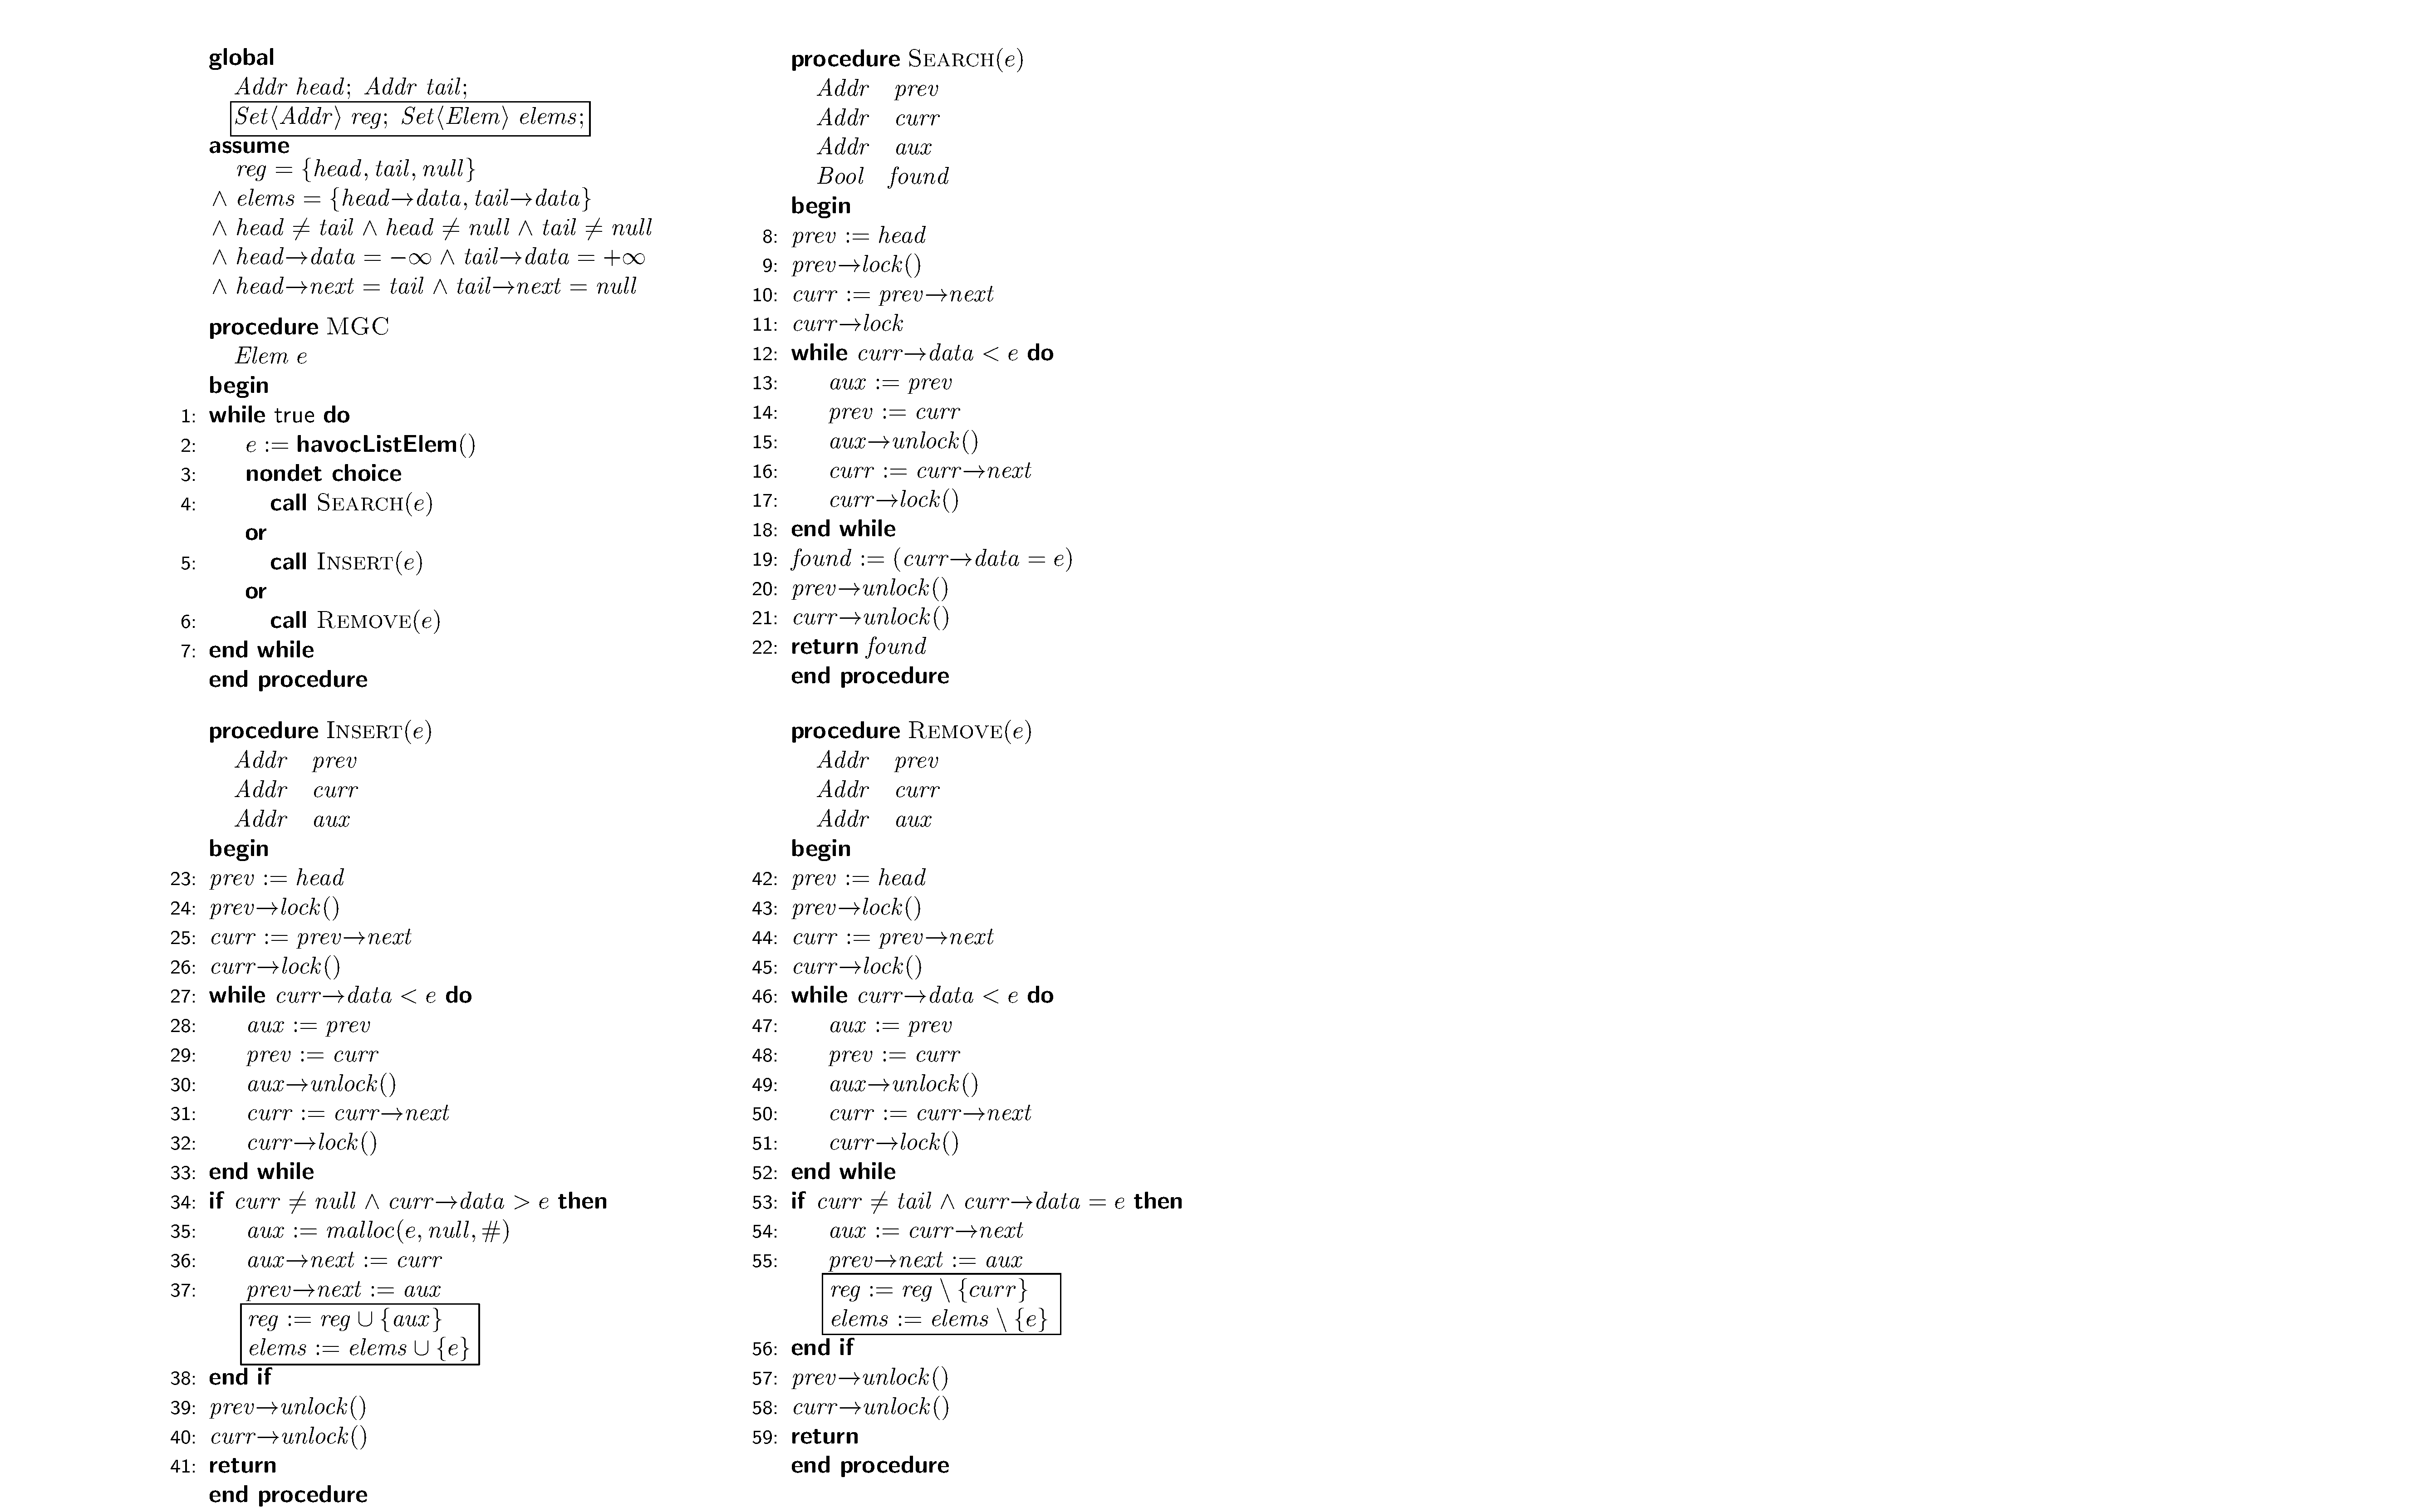
\includegraphics[scale=0.4]{graphics/_listcode}}
		\caption{Concurrent lock-coupling lists implementation.}
		\label{fig:listcode}
\end{figure}
%


\subsection{TL3}
%
\emph{Theory of Linked Lists with Locks} \TLLpL, is the theory we use for describing linked-list heap memory layout.
%
\TLLpL is a multi-sorted first-order theory.
%
It is multi-sorted because it has multiple types for its variables (address, element,...).
%
It is a first-order theory because only variables are quantifiable, as \gls{FOL}.

In this section \TLLpL is defined with the purpose we have. 
%
A more complete and formal definition of \TLLpL can be found in \citeapos{paperAle} and \citep[6.2]{thesisAle}.

Although some functions are originally defined \citep{thesisAle} in suffix notation (\fNext field for instance), preffix-notation has been used to described the theory. 
%
The reason for this modification is to be consistent with \spass syntax.
%
Furthermore, a subset of \TLLpL has been used. 
%
In the same way \gls{FOL} can be expressed with $\neg,\vee$ but sometimes $\implies$ is included but $\dimplies$ is not,
%
few functions have not been used because they can be expressed using others functions in the theory. 
%
We proceed to describe \TLLpL.


\TLLpL is a compound of theories. The \textbf{sorts} used among this theories are: 
%
\cell (representing the nodes of the list),
%
\elem (representing elements),
%
\addr (representing address),
%
\tid (representing thread id),
%
\mem (representing the memory also called heap. It is represented as maps of \addr to \cell ),
%
\path (representing a finite sequence of address),
%
\sSetWhatever (representing a set of \tid,\addr or \elem).

For each sort, there is a theory containing its constants, functions and predicates. 
%
There is one more theory, $\Sigma_{Bridge}$ is a \emph{bridge theory} containing auxiliary
functions, for example, that allow to map paths of addresses to set of 
addresses, or to obtain the set of addresses reachable from a given 
address following a chain of \fNext fields.



\subsection{Signature}

We proceed to describe the signature of each theory, listing the sorts used and explaining its functions, predicates and constants. 
%
Every theory includes the equality theory \ref{theory:equality} 

\todo{\;\;Maybe\;\;these \text{      tables}\;\;should \text{    be reformatted.}}


%%%%%%%%%%%%%%%%%%%%%%%%%%%%%%%%%%%%%%%%%%%%%%%%

%					TID 

%%%%%%%%%%%%%%%%%%%%%%%%%%%%%%%%%%%%%%%%%%%%%%%%
\begin{center}\rule{4cm}{0.4pt} $\Sigma_{\tid}$ \rule{4cm}{0.4pt}\end{center}
%
The sort used is \tid. The "no-thread" value is represented with \fNoThread.
%
Apart from the equality theory, this theory does not have any other predicates or functions.


%%%%%%%%%%%%%%%%%%%%%%%%%%%%%%%%%%%%%%%%%%%%%%%%

%					ELEM

%%%%%%%%%%%%%%%%%%%%%%%%%%%%%%%%%%%%%%%%%%%%%%%%


\begin{center}\rule{4cm}{0.4pt} $\Sigma_{\elem}$ \rule{4cm}{0.4pt}\end{center}
%
The sort used is \elem. 
%
There is a total order which allows to order every set of \elem.
%
In addition, this sort is upper and lower bounded.
%
The signature is described \doubt{in/at} table \ref{table:elem_signature}.


\begin{table}[hbtp]
\centering
\begin{tabular}{rrl}
\fHighest & \elem & Maximum value an \elem can take.\\
\fLowest & \elem & Minimum value an \elem can take.\\
\hline\hline
\fLselem & \elem$\times$\elem & Total order relation between \elem.
\end{tabular}
\caption{\textbf{Signature of $\Sigma_{\ensuremath{\mathit{elem}}}$.} Top block contains functions, lower block contains predicates.}
\label{table:elem_signature}
\end{table}


%%%%%%%%%%%%%%%%%%%%%%%%%%%%%%%%%%%%%%%%%%%%%%%%

%					CELL

%%%%%%%%%%%%%%%%%%%%%%%%%%%%%%%%%%%%%%%%%%%%%%%%

\begin{center}\rule{4cm}{0.4pt} $\Sigma_{\cell}$ \rule{4cm}{0.4pt}\end{center}
%
The sorts used are \cell,\elem,\addr,\tid.
%
The signature is described \doubt{in/at} table \ref{table:cell_signature}.

\begin{table}[hbtp]
\begin{tabular}{rrl}
\fMkcell & $\elem\times\addr\times\tid \to \cell$ & Constructor\\
\fNext & $\cell \to \addr$ & Getter of \fNext field \\ 
\fData & $\cell \to \elem$ & Getter of \fData field \\ 
\fLockID & $\cell \to \tid$ & Getter of \fLockID field \\ 
\fLock & $\cell\times\tid\to\cell$ & Construct a new \cell with \fData and \fNext \\
&&\;\;\;								values of the given \cell, \\
&&\;\;\;				using the \tid for the \fLockID field.\\
\fError & $\cell$ & Constant value used to model \\ 
&&\;\;\;				incorrect memory deference.
\end{tabular}
\caption{\textbf{Functions of $\Sigma_{\cell}$} theory.}
\label{table:cell_signature}
\end{table}

The function \fUnlock could be considered. Actually, \cite{thesisAle} includes it in the theory but it has not been included in this work.
%
The reason is justified because to \fUnlock a \cell is equivalent to \fLock a \cell with \fNoThread value.



%%%%%%%%%%%%%%%%%%%%%%%%%%%%%%%%%%%%%%%%%%%%%%%%

%					MEMORY

%%%%%%%%%%%%%%%%%%%%%%%%%%%%%%%%%%%%%%%%%%%%%%%%


\begin{center}\rule{4cm}{0.4pt} $\Sigma_{\mem}$ \rule{4cm}{0.4pt}\end{center}
%
The sorts used are \mem,\cell and \addr. 
%
The functions are described \doubt{in/at} table \ref{table:memory_signature}.

\begin{table}[hbtp]
\begin{tabular}{rrl}
\fNull & $\addr$ & Null address \\
\fRd & $\mem\times\addr\to\cell$ & Models memory deference. \\
&&								\;\;\; Returns the value from the \mem the \cell \\
&&								\;\;\; stored in the \addr.\\
\fUpd & $\mem\times\addr\times\cell\to\mem$ & Creates a new \mem from the given one\\
\end{tabular}
\caption{\textbf{Functions of $\Sigma_{\mem}$} theory}
\label{table:memory_signature}
\end{table}

A function related with \mem theory is \fMalloc, used in \insertprg procedure.
%
\fMalloc is a function which does not belongs to \gls{SPL} nor \TLLpL but it can be translated as a conjecture of assignations and assignations are allowed in both theories.
%
\fMalloc returns a new fresh address different to every other address in use, so the \freshaddr returned by \fMalloc is not equal to \head, nor \tail, etc.
%
\fMalloc formal representation correspond to a big conjecture of all the formulas stating \freshaddr is not equal to \addr, for all \addr appearing in the formula (except itself).


%%%%%%%%%%%%%%%%%%%%%%%%%%%%%%%%%%%%%%%%%%%%%%%%

%					SETADDR

%%%%%%%%%%%%%%%%%%%%%%%%%%%%%%%%%%%%%%%%%%%%%%%%


\begin{center}\rule{4cm}{0.4pt} $\Sigma_{\sSetAddr}$ \rule{4cm}{0.4pt}\end{center}
%
It models the usual set theory. 
%
Preffix version of each function and predicate has been preferred to be consistent with \ref{ax::fulllist}.
%
The signature is described \doubt{in/at} table \ref{table:setaddr_signature}.

Intersection function and subset predicate has not been included despite \citep{thesisAle} uses them. 
%
They were not used because they were unnecessary.

\begin{table}[hbtp]
\begin{tabular}{rrl}
\fEmptyset & \sSetAddr & Empty set\\
\fSingl & $\addr\to\sSetAddr $& Constructor of a single-element set.\\
\fUnion & $\sSetAddr\times\sSetAddr\to\sSetAddr$&\\
\fSetdiff & $\sSetAddr\times\sSetAddr\to\sSetAddr$&\\
\hline\hline
\pIn & $\sAddr\times\sSetAddr $& \\
\end{tabular}
\caption{\textbf{Signature of $\Sigma_{\sSetAddr}$.} Top block contains functions, lower block contains predicates.}
\label{table:setaddr_signature}
\end{table}


%%%%%%%%%%%%%%%%%%%%%%%%%%%%%%%%%%%%%%%%%%%%%%%%

%					SETELEM

%%%%%%%%%%%%%%%%%%%%%%%%%%%%%%%%%%%%%%%%%%%%%%%%


\begin{center}\rule{4cm}{0.4pt} $\Sigma_{\sSetElem}$ \rule{4cm}{0.4pt}\end{center}
%

Again, it models the usual set theory.
%
The signature is described \doubt{in/at} table \ref{table:setelem_signature}.

\begin{table}[hbtp]
\begin{tabular}{rrl}
\fEmptysetElem & $\sSet $& Empty set\\
\fSinglElem & $\elem\to\sSet $& Constructor of a single-element set.\\
\fUnionElem & $\sSet\times\sSet\to\sSet$&\\
\fSetdiffElem & $\sSet\times\sSet\to\sSet$&\\
\hline\hline
\pInElem & $\sAddr\times\sSet $& \\
\end{tabular}
\caption{\textbf{Signature of $\Sigma_{\sSetElem}$.} Top block contains functions, lower block contains predicates.}
\label{table:setelem_signature}
\end{table}


%%%%%%%%%%%%%%%%%%%%%%%%%%%%%%%%%%%%%%%%%%%%%%%%

%					SETTID

%%%%%%%%%%%%%%%%%%%%%%%%%%%%%%%%%%%%%%%%%%%%%%%%


\begin{center}\rule{4cm}{0.4pt} $\Sigma_{\sSetTid}$ \rule{4cm}{0.4pt}\end{center}
%


The signature is described \doubt{in/at} table \ref{table:settid_signature}.

\begin{table}[hbtp]
\begin{tabular}{rrl}
\fEmptysetTid & $\sSetAddr $& Empty set\\
\fSinglTid & $\addr\to\sSetAddr $& Constructor of a single-element set.\\
\fUnionTid & $\sSetAddr\times\sSetAddr\to\sSetAddr$&\\
\fSetdiffTid & $\sSetAddr\times\sSetAddr\to\sSetAddr$&\\
\hline\hline
\pInTid & $\sAddr\times\sSetAddr$ &\\
\end{tabular}
\caption{\textbf{Signature of $\Sigma_{\sSetAddr}$.} Top block contains functions, lower block contains predicates.}
\label{table:settid_signature}
\end{table}




%%%%%%%%%%%%%%%%%%%%%%%%%%%%%%%%%%%%%%%%%%%%%%%%

%					BRIDGE

%%%%%%%%%%%%%%%%%%%%%%%%%%%%%%%%%%%%%%%%%%%%%%%%


\begin{center}\rule{4cm}{0.4pt} $\Sigma_{Bridge}$ \rule{4cm}{0.4pt}\end{center}
%

This theory is much more extensive \doubt{in/on/at} \cite{thesisAle}. 
%
However, aiming to simplicity, not every function and predicate described there has been used in our proofs.
%
We include in the signature described \doubt{in/at} table \ref{table:bridge_signature} the functions and predicates used in the proofs.

\begin{table}[hbtp]
\begin{tabular}{rrl}
\fAddrToSet & $\mem\times\addr\to\sSetAddr $& Returns the set of \addr reachable from the \addr given.\\
\hline\hline
\end{tabular}
\caption{\textbf{Signature of $\Sigma_{\sSetAddr}$.}}
\label{table:bridge_signature}
\end{table}





%
% Desarrollo
%
% -*- root: ../main.tex -*-
\chapter{Development\label{sec:develpment}}

\paragraph{Abstract} 

In this chapter, we describe the practical work.
%
Until now, we just have defined the theoretical foundations.

Here we will expose the rigorous methodology used to mathematically perform our verification.
%
To achieve our goals, we have developed some tools which are described here too.

We will end the chapter defining precisely the goal and the logic formulas needed to prove valid in order to claim that the program is verified.

\section{Methodology Used}

\subsection{Process, Tools Used and Tools Developed}

\subsubsection{Spass}

\spass \cite{spass} is an automated theorem prover for first-order logic with equality. 
%
\spass receives a \gls{FOL} formula and tries to prove it valid.
% 
Running SPASS on such a formula results in the final output “\textit{SPASS beiseite: Proof found.}” if the formula is valid or  “\textit{SPASS beiseite: Completion found.}” if the formula is not valid.
%
Because validity in first-order logic is undecidable, SPASS may run forever without producing any final result.
%
This last comment is a very important issue because some proofs have taken hours and one could not know for sure if \spass would eventually stop or run forever.
%
As a curiosity, the longest time \spass was left running was 82 hours and it stopped because a proof was found.

%At appendix \ref{spass:syntax_file} an example of a complete \spass file can be found.

\subsubsection{Leap}

\leap is a tool for the verification of concurrent data types and parametrized systems executed by an unbounded number of threads which manipulate mutable shared data in the heap.

Leap receives as input a concurrent program description and a specification and automatically generates a finite set of verification conditions which are then discharged to specialized decision procedures. 
%
The validity of all discharged verification conditions implies that the program executed by any number of threads satisfies the specification. 
%
Currently, Leap includes not only decision procedures for integers and Booleans, but it also implements specific theories for heap memory layouts such as linked-lists and skiplists.


\subsubsection{\gandalf}

\gandalf is a tool implemented  as part of this project to aid \spass proving \gls{VC}. 
%
\gandalf implements the process of converting the VCs generated by \leap to \spass syntax, splitting different conjunctions in different files, calling \spass to try to prove and process and storing the results has been automatized basically in python combined with bash scripts.
%
Additionally, \spass reads prefix syntax while \leap uses prefix and infix syntax.

In addition, \gandalf does some reduction of the formulas so \spass can finish in a reasonable time.
%
This is needed because \spass does not use any information or tactics to decide which axiom should be used first.


\subsubsection{Process of Tool Cooperation}

\label{ProcessDescription}
We describe now the way in which the tools cooperate.
%
The process followed is shown in Fig. \ref{fig:process}


\begin{figure}
\tikzset{
    vertex/.style = {
        circle,
        fill            = black,
        outer sep = 2pt,
        inner sep = 1pt,
    }
}

\begin{tikzpicture}[scale=2]
\newcommand{\initiation}{Initiation}
\newcommand{\selfconsec}{Self consecution}
\newcommand{\otherconsec}{Others consecution}
\newcommand{\valid}{Valid}
  % Dialectics
  \node[draw] (ProgramName) at (1.5,1.5) {Invariant};
  \node (Program) at (1.85,1.5) {};
  
  \node[draw,minimum width=1.2cm, minimum height=0.5cm] (VC1) at (3,3.8) {$VC_1$};
  


  \node[draw,minimum width=1.2cm, minimum height=0.5cm] (VC21) at (3,2.8) {$VC_{2-1}$};
  \node[draw,minimum width=1.2cm, minimum height=0.5cm] (VC22) at (3,2.2) {$VC_{2-2}$};
  \node[draw,minimum width=1.2cm, minimum height=0.5cm] (VC3) at (3,1.0) {$\vdots$};
  \node[draw,minimum width=1.2cm, minimum height=0.5cm] (VC55-1) at (3,0.3) {$VC_{55-1}$};
  \node[draw,minimum width=1.2cm, minimum height=0.5cm] (VC55-2) at (3,-0.4) {$VC_{55-2}$};

  \node[draw,text=white,fill=gray,minimum width=4.2cm, minimum height=0.9cm] (Ax) at (8.4,5) {\large{\textbf{List of axioms}}};
  \node[draw,text=black,fill=green] (AxCons) at (4,5) {\textbf{Trustful}};
  \draw[-] (Ax) to node[above] {parser \& leap} (AxCons);
  %\draw[->] (Ax) to node[above] {parser and leap} (AxCons);

  %%%%%%%%%%%%%%%%% Gandalf Generation
 %\newcommand{\smallToBig}{Ola} 
  \node[draw,minimum width=5.4cm,minimum height = 0.5cm] (SP11) at (5.5,4.2) {$\tau_1$ - \initiation};
  
  \node[draw,minimum width=5.4cm,minimum height = 0.5cm] (SP21) at    (5.5,3.6) {$\tau_2$ - \selfconsec};
  \node[draw,minimum width=5.4cm,minimum height = 0.5cm,fill=black!10!white] (SP21_f) at  (5.5,3.3) {\smallToBig};

  \node[draw,minimum width=5.4cm,minimum height = 0.5cm] (SP221) at   (5.5,2.8) {$\tau_2$ - \otherconsec (1)};
  \node[draw,minimum width=5.4cm,minimum height = 0.5cm] (SP222) at   (5.5,2.4) {$\dots$};
  \node[draw,minimum width=5.4cm,minimum height = 0.5cm] (SP22n) at   (5.5,2.0) {$\tau_{55}$ - \otherconsec (55)};
  \node[draw,minimum width=5.4cm,minimum height = 0.5cm,fill=black!10!white] (SP22n_f) at (5.5,1.6) {\smallToBig};

  \node[draw,minimum width=5.4cm,minimum height = 0.5cm] (SP31) at    (5.5,1.1) {$...$};
  \node[draw,minimum width=5.4cm,minimum height = 0.5cm,fill=black!10!white] (SP31_f) at  (5.5,0.8) {\smallToBig};

  \node[draw,minimum width=5.4cm,minimum height = 0.5cm] (SP55-1) at  (5.5,0.3) {$\tau_{55}$ - \selfconsec};
  \node[draw,minimum width=5.4cm,minimum height = 0.5cm,fill=black!10!white] (SP55-1_f) at (5.5,0) {\smallToBig};
  
  \node[draw,minimum width=5.4cm,minimum height = 0.5cm] (SP55-2) at   (5.5,-0.5) {$\tau_{55}$ - \otherconsec};
  \node[draw,minimum width=5.4cm,minimum height = 0.5cm,fill=black!10!white] (SP55-2_f) at (5.5,-0.8) {\smallToBig};
  
  \node (SP11_p) at (4.25,4.2) {};

  \node (SP21_p) at    (4.25,3.6)  {};
  \node (SP21_f_p) at  (4.25,3.3)  {};

  \node (SP221_p) at   (4.25,2.8)  {};
  %%\node (SP221_f_p) at (4.25,2.5)  {};
  
  \node (SP222_p) at   (4.25,2.4)  {};
  %%\node (SP222_f_p) at (4.25,1.7)  {};

  \node (SP22n_p) at   (4.25,2.0)  {};
  \node (SP22n_f_p) at (4.25,1.6)  {};

  \node (SP31_p) at    (4.25,1.1)  {};
  \node (SP31_f_p) at  (4.25,0.8)  {};

  \node (SP55-1_p) at  (4.25,0.3) {};
  \node (SP55-1_f_p) at (4.25,0) {};
  
  \node (SP55-2_p) at   (4.25,-0.5) {};
  \node (SP55-2_f_p) at (4.25,-0.8) {};
  




  

  
   \node[draw,fill=green] (True11) at (9,4.2) {\valid};
  
   \node[draw,fill=green] (True21) at (9,3.6) {\valid};
   \node[draw,fill=green] (True21_f) at (9,3.3) {\valid};

   \node[draw,fill=green] (True221) at (9,2.8) {\valid};
   \node[draw,fill=green] (True222) at (9,2.4) {\valid};
   \node[draw,fill=green] (True22n) at (9,2.0) {\valid};
   \node[draw,fill=green] (True22n_f) at (9,1.6) {\valid};

   \node[draw,fill=green] (True31) at (9,1.1) {\valid};
   \node[draw,fill=green] (True31_f) at (9,0.8) {\valid};

   \node[draw,fill=green] (True55-1) at (9,0.3) {\valid};
   \node[draw,fill=green] (True55-1_f) at (9,0) {\valid};
  
   \node[draw,fill=green] (True55-2) at (9,-0.5) {\valid};
   \node[draw,fill=green] (True55-2_f) at (9,-0.8) {\valid};

  
  
  %%%%%%%%%%%%%%%%%%%%%% 			 %%%%%%%%%%%%%%%%%%%%%%   
  %%%%%%%%%%%%%%%%%%%%%% TRANSITIONS %%%%%%%%%%%%%%%%%%%%%%
  %%%%%%%%%%%%%%%%%%%%%% 			 %%%%%%%%%%%%%%%%%%%%%% 

  \draw[->,draw=blue] (Program) to node[pos=0.3,above] {\leap} (VC1);
  \draw[->,draw=blue] (Program) to node[pos=0.4,above] {} (VC21);
  \draw[->,draw=blue] (Program) to node[pos=0.4,above] {} (VC22);
  \draw[->,draw=blue] (Program) to node[pos=0.4,above] {} (VC3);
  \draw[->,draw=blue] (Program) to node[pos=0.4,above] {} (VC55-1);
  \draw[->,draw=blue] (Program) to node[pos=0.4,above] {} (VC55-2);
  
 	
  \draw[->,draw=blue] (VC1) to node[above,pos=0.4] {\gandalf} (SP11_p);
  
  \draw[->,draw=blue] (VC21) to node[above,pos=0.4] {\gandalf} (SP21_p);
  \draw[->,draw=blue] (VC22) to node[above,pos=0.4] {\gandalf} (SP221_p);
  \draw[->,draw=blue] (VC22) to node[above,pos=0.4] {} (SP222_p);
  \draw[->,draw=blue] (VC22) to node[above,pos=0.4] {} (SP22n_p);
  
  \draw[->,draw=blue] (VC3) to node[above,pos=0.4] {\gandalf} (SP31_p);
  
  \draw[->,draw=blue] (VC55-1) to node[above,pos=0.4] {\gandalf} (SP55-1_p);
  \draw[->,draw=blue] (VC55-2) to node[above,pos=0.4] {\gandalf} (SP55-2_p);

  
 	%%% small to big
 	\draw[->,draw=blue] (VC21) to node[above,pos=0.4] {} (SP21_f_p);
  %\draw[->,draw=blue] (VC22) to node[above,pos=0.4] {} (SP221_f_p);
  %\draw[->,draw=blue] (VC22) to node[above,pos=0.4] {} (SP222_f_p);
	\draw[->,draw=blue] (VC22) to node[above,pos=0.4] {} (SP22n_f_p);
	
 	\draw[->,draw=blue] (VC3) to node[above,pos=0.4] {} (SP31_f_p);
	
 	\draw[->,draw=blue] (VC55-1) to node[above,pos=0.4] {} (SP55-1_f_p);
	\draw[->,draw=blue] (VC55-2) to node[above,pos=0.4] {} (SP55-2_f_p);

	

	

  	
  	\draw[->] (SP11) to node[above,pos=0.4] {\textbf{\spass}} (True11);
    
    \draw[->] (SP21) to node[above,pos=0.4] {\textbf{\spass}} (True21);
    \draw[->] (SP221) to node[above,pos=0.4] {\textbf{\spass}} (True221);
    \draw[->] (SP222) to node[above,pos=0.4] {\textbf{\spass}} (True222);
    \draw[->] (SP22n) to node[above,pos=0.4] {\textbf{\spass}} (True22n);
    
    
    \draw[->] (SP31) to node[above,pos=0.4] {\textbf{\spass}} (True31);
    
    \draw[->] (SP55-1) to node[above,pos=0.4] {\textbf{\spass}} (True55-1);
    \draw[->] (SP55-2) to node[above,pos=0.4] {\textbf{\spass}} (True55-2);
  
    %\draw[->] (SP11_f) to node[above,pos=0.4] {\textbf{\spass}} (True11_f);
  	
  	\draw[->] (SP21_f) to node[above,pos=0.4] {\textbf{\spass}} (True21_f);
    %\draw[->] (SP221_f) to node[above,pos=0.4] {\textbf{\spass}} (True221_f);
    %\draw[->] (SP222_f) to node[above,pos=0.4] {\textbf{\spass}} (True222_f);
  	\draw[->] (SP22n_f) to node[above,pos=0.4] {\textbf{\spass}} (True22n_f);
  	
  	
  	\draw[->] (SP31_f) to node[above,pos=0.4] {\textbf{\spass}} (True31_f);
  	
  	\draw[->] (SP55-1_f) to node[above,pos=0.4] {\textbf{\spass}} (True55-1_f);
  	\draw[->] (SP55-2_f) to node[above,pos=0.4] {\textbf{\spass}} (True55-2_f);
  


  \draw[-,draw=blue](Ax) to (8.4,-0.8);	



  
   \draw node[vertex] (Joint) at (8.4,4.2) {};
  
   \draw node[vertex] (Joint) at (8.4,3.6) {};
   \draw node[vertex] (Joint) at (8.4,3.3) {};

   \draw node[vertex] (Joint) at (8.4,2.8) {};
   \draw node[vertex] (Joint) at (8.4,2.4) {};
   \draw node[vertex] (Joint) at (8.4,2.0) {};
   \draw node[vertex] (Joint) at (8.4,1.6) {};

   \draw node[vertex] (Joint) at (8.4,1.1) {};
   \draw node[vertex] (Joint) at (8.4,0.8) {};

   \draw node[vertex] (Joint) at (8.4,0.3) {};
   \draw node[vertex] (Joint) at (8.4,0) {};
  
   \draw node[vertex] (Joint) at (8.4,-0.5) {};
   \draw node[vertex] (Joint) at (8.4,-0.8) {};


  %	\draw node[vertex] (Joint) at (7.4,4.2) {};
  % \draw node[vertex] (Joint) at (7.4,3.6) {};
  %	\draw node[vertex] (Joint) at (7.4,3.0) {};
  %	\draw node[vertex] (Joint) at (7.4,2.4) {};
  %	\draw node[vertex] (Joint) at (7.4,1.8) {};
  %	\draw node[vertex] (Joint) at (7.4,1.2) {};
  %	\draw node[vertex] (Joint) at (7.4,0.5) {};
  %	\draw node[vertex] (Joint) at (7.4,-0.2) {};
  %	\draw node[vertex] (Joint) at (7.4,-0.8) {};
  % \draw node[vertex] (Joint) at (7.4,-1.4) {};


  %\draw[->,draw=blue] (Joint) to (Synthesis);
  %\draw[->,draw=blue] (Synthesis) to[in=180,out=180] (Thesis);
  
  \draw[-,thick] (1,-2) -- (8,-2);
    \node (Program2) at (4.5,-2.5) {Program};
    \node[fill=green] (Final) at (5.5,-2.5) {\valid};
    \node (equiv) at (5,-2.5) {$\equiv$};
     


  
  \end{tikzpicture}
\caption{Process graph}
\label{fig:process}
\end{figure}

The first step consists on translating the program into \gls{VC}. 
%
This is done by \leap. 
%
In the case of verifying single linked list, \leap generates at least 2 \gls{VC} for each transition of the program. 
%
The first \gls{VC} corresponds to self-consecution, and the second corresponds to others-consecution.
%
The initial transition is also generated.
%
The process is repeated 6 times, one for each candidate invariant of the problem (\ref{invariants}).

Once the \gls{VC}s have been generated, the goal is to prove all of them using \spass. 
%
As the syntax of \spass (\cite{spasssyntax}) is not \leap syntax some parsing is needed. 
%
For example, \spass uses prefix notation  \leap uses infix notation for binary functions.
%
In order to solve this, it was necessary to learn \ocaml using \citeapos{ocamlbook}.
%
\leap was forked so it could write the \gls{VC}s in prefix notation.
%
Some other \leap functionalities had to be changed to make \leap output compatible with \spass input.

In addition, one \spass problem has to be created for each \gls{VC}. 
%
The axiom list for each problem is determined as an argument. 
%
This is explained further in section \ref{sec:axiomgraph}.

Because of \spass lacks of tactics and the relatively large size of the axiom list, some very easy proofs could take a long time.
%
For transitions which can be proven using very simple reasoning using \pc s,\spass could take minutes. 
%
In order to improve \spass performance, we decided to divide the problem upfront.

Let $\varphi$ be the \gls{VC} to prove. Consider for example the following \gls{VC}
	\[
		\varphi : \;\;\;\;\; \pc(i) = l_j \to \head \not = \tail
	\]
While proving the \gls{VC} for the thread $i$, $\pc(i)$ has a value which may be $l_j$ or not. 
%
In both cases, resolution can be applied to prove equivalently
	\[
		\psi : \;\;\;\;\; \head \not = \tail
	\]
This resolution can be applied in self-consecution and in others-consecution. 
%
This resolution step is done by \gandalf. 
%
Some other obvious resolution is also performance at this stage, such as $\top \andcond \top \equiv \top$ and other tautologies.

Now \spass can prove a simpler problem requiring much less time.
%
To make sure that both problem are equivalent and that the conversion was sound, we generate another \spass problem. 
%
This \spass problem aims to prove $\psi \to \varphi$.
%
In order to prove $\varphi$, modus ponens is used:
\[
	\begin{array}{l}
		\psi\\
		\psi \to \varphi\\\hline
		\varphi
	\end{array}
\]

Even though two \spass problems have to be solved instead of one, in \ref{sec:timeanalysis} the reader can see the benefits of applying this method.
%
The reason is that $\varphi$ is a complex problem for \spass. 
%
However, $\psi$ is a much simpler problem because it does not include any reasoning about program counters. 
% How to express:
%%%%    I didn't check that is tautologic in every transition, but i am pretty sure it is.
In addition, the problem $\psi \to \varphi$ is tautologic in most of the transitions because it adds conjectures in the antecedent of an implication, which cannot make invalid a valid formula.
%
Plus, the list of axioms needed to prove $\ps$ is smaller where compared to the axiom list needed to prove the original problem.


The generated problem $\psi$ will be called the \textbf{\reducedProblem} and $(\psi \to \varphi)$ will be called the \textbf{\smallToBig}. $\varphi$ problem will be called the \textbf{\originalProblem}

The \reducedProblem  should not have any $\pc$ involved. How can the $\pc$ be removed while proving others-consecution?
%
Again, more \spass problems are generated. 
%
In this case, 55 new problems are generated and using modus ponens:
\[
	\begin{array}{l}
		\psi_1\\
		\psi_2\\
		\vdots\\
		\psi_{55}\\
		(\bigwedge_i \psi_i) \to \varphi\\\hline
		\varphi
	\end{array}
\]
%%%%    I didn't check that is tautologic in every transition, but i am pretty sure it is.
In this case again, the \spass problem $(\bigwedge_i \psi_i) \to \varphi$ is tautologic most of the time, but \spass takes much more time than before because of the problem size.




\subsection{Auxiliary Tools}
\subsubsection{\ocaml - parser}
All the process described above require an axiom list. 
%
Getting the axioms needed to prove all the transitions was the most difficult work. 
%
Typically, we provided \spass with an axiom list with which all \gls{VC}s were proven. In the process of checking the generated proofs and verify they were correct, we found some inconsistencies. 
%
This inconsistencies were always consequence of incorrect axioms. 
%
Because of human ingenuity, it was very difficult to ensure absolute validity of the axioms.\footnote{Axioms should be universally valid (not just valid in \TLLpL theory) so they could be used for other theories that \leap can work with.}
%
In order to solve this, we decided to validate every axiom using \leap. 
%
This procedure does not assure absolute validity to the axioms but helped a lot to find incomplete axioms.

As there are several axioms, a parser was implemented to automatize the parsing files from \spass syntax to \leap. 
%
The parser was implemented in \ocaml so \ocaml skills could be improved. Additionally, \citetool{ocamllex} and \citetool{ocamlyacc}, \ocaml variants of the \mbox{C} tools studied during the bachelor degree (\textit{Proyecto de Autómatas y Lenguajes}) have been used to implement the parser.
%
The functionality of translating from \spass syntax to \LaTeX\; syntax has also been included to generate the axiom list \ref{ax::fulllist}



\section{Linked list}
%
We manage to prove that the implementation proposed at \ref{fig:listcode} of a concurrent lock coupling linked-list always preserves the list structure. 
%
There are some conditions to assure that a set of nodes is a list.
%
An order has to be preserved, \head and \tail must keep the properties of its definition. 
%
We gather all the necessary conditions in formula (\ref{inv:list}):


	\begin{align}
	  	\invPreserve & \overset{\mbox{def}}{=} \formulaFullListReducedBody
	  	\label{inv:list}
	\end{align}

(L1) establishes that \fNull is in \region and that \region is
exactly the set of addresses reachable in the \heap starting from
\head, which ensures that the list is not circular.
%
(L2) and (L3) express some sanity properties of the sentinel nodes
\head and \tail.
%
Finally, (L4) express the fact that the list is ordered.

We claim that the formula \invPreserve is an invariant of this implementation. The full proof can be found later in \ref{proof:Preserve}. 
%
Although this may seem easy, human ingenuity makes it hard. 
%
In \citeapos{tempVerifLinkedList} the authors whoen that \invPreserve is not an inductive invariant. 
%
We need others invariants as support.

\subsubsection{Invariants of the implementation}
\label{invariants}
As these are not principal but auxiliary invariants, we just provided here a brief description of them.
%
These auxiliary invariants are needed to prove \invPreserve and 
%
a full description of each formula appear in \ref{appendix::inv:full}.
%
%
%
%
\paragraph{\invDisjoint:}
This invariants provides the information needed when inserting a new element.
%
Two different \fMallocc invocations return two different addresses, so there is not possible to insert the same address twice in the list.
%
\paragraph{\invRegion:}
These invariants refers to the information about to which addresses are in the ghost variable \region var, that is, which addresses are reachable from \head.
%
\paragraph{\invLock:}
These invariants refer to the information provided by the locks. 
%
The \fLock acquired at line $l_i$ is not unlocked until line $l_{i+j}$, so at lines $l_{k}\; k\in(i,i+j)$ the \fLock should be locked by the running thread.
%
This is a very important invariant because it assures that concurrent access are safe and therefore it is well implemented.
%
\paragraph{\invOrder:}
These invariants refer to the information related to the order of the list. 
%
\paragraph{\invNext:}
These invariants refer to the information provided by \fNext statements. 
%
If at $l_i$, $\curr := \prev\to\fNext()$, is executed $\curr$ still has the value $\prev$ until a new assignment to $\curr$ is done.
%
This invariant encodes the information about the relation between addresses.

\subsubsection{Dependencies between invariants}
The only inductive invariant is \invOrder. 
%
The rest of the auxiliary invariants need some other invariants to prove them.
%
In figure \ref{fig:proofgraph} the graph of dependencies is shown.
%
As it is shown, the invariant \invDisjoint is not directly needed to proof \invPreserve, but it is needed as support to proof both \invNext and \invRegion. 

\begin{center}
\includegraphics[scale=0.5]{graphics/proofgraph_lists.pdf}
\label{fig:proofgraph}
\end{center}

One could think that it is not sound to prove \invLock using \invRegion as support and prove \invRegion using \invLock as support.
%
\todo{\;\;Why\;it\;is\;not \text{   cheating?}}


%
% Resultados
%
\chapter{Results\label{chap:results}}

\section{Analysis of generated proofs}

\subsection{Special transitions}

\section{Time analysis}

\subsection{Proof generation}

\subsection{Proof checking}


\subsection{Leap times}




%
% Conclusiones
%
\chapter{Conclusions\label{sec:conclusiones}}

\section{Linked list theory axiomatizable}

\section{Refutation worth it}

\subsection{Spass Time compared to leap}

 



%
% Página en blanco
%
\cleardoublepage

%
% Bibliografía
%
\printbibliography[heading=bibintoc]

% No expandir elementos para llenar toda la página
\raggedbottom

\printindex
%
% Apéndices
%
\appendix
\cleardoublepage
\addappheadtotoc
\appendixpage

%
% TODO: Apéndices del TFG
%
\include{src/appendixExample}

% Fin del documento


\end{document}
